\chapter{Cơ sở lý thuyết}
Để giải quyết hiệu quả bài toán tái tạo mô hình 3D chi tiết và chính xác cho cột ăng-ten của trạm viễn thông, chương này sẽ trình bày một cách hệ thống các kiến thức lý thuyết nền tảng và các công trình nghiên cứu liên quan. Trong đó, một số kiến thức cơ bản về luồng thực hiện tái tạo đám mây điểm 3D và các thuật toán trích xuất đặc trưng dựa trên học sâu liên quan sẽ được trình bày chi tiết.
% \section{Giới thiệu về máy ảnh}

Máy ảnh (không làm thay đổi tính chất kỹ thuật, sau đây sử dụng từ "máy ảnh" để thay thế) là một thiết bị cơ bản trong thị giác máy tính, đóng vai trò thu thập dữ liệu hình ảnh từ thế giới thực. Để có thể sử dụng hình ảnh này cho các tác vụ phân tích và tái tạo 3D, chúng ta cần hiểu rõ về các đặc tính và mô hình của máy ảnh. Các đặc tính này thường được chia thành hai nhóm chính: tham số nội tại (gọi là  intrinsic) và tham số ngoài (gọi là extrinsic).

\subsection{Mô hình máy ảnh pinhole}
\label{subsec:pinhole_máy ảnh}

Mô hình máy ảnh pinhole là một mô hình hình học lý tưởng hóa, đơn giản nhất để mô tả quá trình tạo ảnh của một máy ảnh. Mặc dù bỏ qua các hiệu ứng quang học phức tạp của thấu kính thật (như méo ảnh, độ sâu trường ảnh), mô hình này lại là nền tảng toán học cốt lõi cho hầu hết các thuật toán trong thị giác máy tính và phục dựng 3D. Nó cung cấp một mối quan hệ hình học rõ ràng giữa các điểm 3D trong không gian và hình chiếu 2D của chúng trên mặt phẳng ảnh.

Các thành phần chính của mô hình máy ảnh pinhole bao gồm (xem Hình \ref{fig:pinhole_model}):
\begin{itemize}
    \item \textbf{Tâm quang học (Optical Center) hay Tâm chiếu (Center of Projection), $\vect{O}$}: Điểm duy nhất trong không gian mà tất cả các tia sáng từ vật thể đi qua trước khi tạo thành ảnh. Nó tương ứng với "pinhole" lý tưởng.
    \item \textbf{Mặt phẳng ảnh (Image Plane)}: Một mặt phẳng đặt vuông góc với trục quang học và cách tâm quang học $\vect{O}$ một khoảng bằng tiêu cự $f$. Đây là nơi hình ảnh của cảnh được hình thành. Trong máy ảnh thực tế, đây chính là bề mặt của cảm biến ảnh (sensor).
    \item \textbf{Trục quang học (Principal Axis)}: Đường thẳng đi qua tâm quang học $\vect{O}$ và vuông góc với mặt phẳng ảnh.
    \item \textbf{Điểm chính (Principal Point), $\vect{c}$}: Giao điểm của trục quang học với mặt phẳng ảnh. Trong mô hình lý tưởng, nó thường được giả định là nằm ở tâm của mặt phẳng ảnh/cảm biến.
    \item \textbf{Tiêu cự (Focal Length), $f$}: Khoảng cách từ tâm quang học $\vect{O}$ đến mặt phẳng ảnh dọc theo trục quang học.
\end{itemize}

\subsubsection{Phép chiếu phối cảnh (Perspective Projection)}

Trong mô hình máy ảnh pinhole, một điểm 3D $\vect{X}$ trong không gian được chiếu lên mặt phẳng ảnh thành một điểm ảnh 2D $\vect{x}'$ thông qua một phép chiếu gọi là **phép chiếu phối cảnh (perspective projection)**. Phép chiếu này tuân theo nguyên tắc đường thẳng: hình chiếu $\vect{x}'$ là giao điểm của tia sáng đi từ $\vect{X}$ qua tâm quang học $\vect{O}$ với mặt phẳng ảnh.

Do tia sáng đi qua tâm quang học, hình ảnh được tạo ra trên mặt phẳng ảnh đặt phía sau $\vect{O}$ sẽ bị lộn ngược (cả chiều trên-dưới và trái-phải) so với vật thể thực. Để thuận tiện cho việc phân tích toán học, người ta thường xem xét một **mặt phẳng ảnh ảo (virtual image plane)** đặt ở phía trước tâm quang học $\vect{O}$, cũng cách $\vect{O}$ một khoảng $f$ và song song với mặt phẳng ảnh thực. Hình chiếu $\vect{x}$ trên mặt phẳng ảnh ảo này sẽ cùng chiều và không bị lật so với vật thể (Hình \ref{fig:pinhole_model}). Các phân tích hình học sau đây thường dựa trên mặt phẳng ảnh ảo này.

% --- Hình ảnh minh họa ---
\begin{figure}[H] % [H] để ép ảnh hiển thị ngay tại vị trí code (cần gói float)
    \centering
    \begin{tikzpicture}[scale=0.9, >=stealth]
        % Hệ tọa độ máy ảnh (Xc, Yc, Zc)
        \coordinate (O) at (0,0); % Tâm quang học
        \draw[->, thick] (O) -- (4,0) node[below left] {$Z_c$}; % Trục Zc (trục quang học)
        \draw[->, thick] (O) -- (0,2.5) node[right] {$Y_c$}; % Trục Yc
        \draw[->, thick] (O) -- (-1.5,-1) node[below] {$X_c$}; % Trục Xc
        \fill (O) circle (1.5pt) node[below left] {$\vect{O}$};

        % Mặt phẳng ảnh ảo (tại Z=f)
        \def\focal{2} % Tiêu cự f
        \coordinate (c) at (\focal, 0); % Điểm chính
        \fill (c) circle (1pt) node[below] {$\vect{c}$};
        \draw[dashed, blue] (\focal, -1.5*1.2) -- (\focal, 1.5*1.2); % Đường trục y ảnh
        \draw[dashed, blue] (\focal-0.6*1.2, -0.4*1.2) -- (\focal+0.6*1.2, 0.4*1.2); % Đường trục x ảnh (xiên)
        \node[blue, above right] at (\focal+0.6*1.2, 0.4*1.2) {Image Plane ($\pi$)};
        \draw[<->] (O) -- (c) node[midway, above] {$f$};

        % Điểm 3D trong hệ tọa độ máy ảnh Xc
        \coordinate (Xc) at (3.5, 1.5);
        \coordinate (Xc_proj_xy) at (3.5, 0);
        \coordinate (Xc_proj_xz) at (3.5, 0, 1.5); % Giả định tọa độ x (chiều sâu khác)
        \fill (Xc) circle (1.5pt) node[above right] {$\vect{X}_c=(X_c, Y_c, Z_c)$};
        \draw[dotted] (Xc) -- (Xc_proj_xy);
        \node[right] at (Xc_proj_xy) {$Z_c$};
        \draw[dotted] (Xc) -- (0, 1.5);
        \node[above] at (0, 1.5) {$Y_c$};
        % Vẽ thêm chiếu lên mặt XZ nếu cần

        % Tia chiếu từ Xc qua O
        \draw[red, thick] (Xc) -- (O);

        % Giao điểm với mặt phẳng ảnh ảo (x)
        \path[name path=ray] (Xc) -- (O);
        \path[name path=image_plane] (\focal, -2) -- (\focal, 2); % Đường dài hơn để chắc chắn cắt
        \path[name intersections={of=ray and image_plane, by=x_proj}];
        \fill[red] (x_proj) circle (1.5pt) node[below right, red] {$\vect{x}=(x,y)$};
        \draw[dotted] (x_proj) -- (c); % Chiếu xuống trục Zc
        \draw[dotted] (x_proj) -- (\focal, 1.5*\focal/3.5); % Chiếu ngang sang trục Y ảnh ảo

        % Tam giác đồng dạng
        \draw[gray] (O) -- (Xc) -- (3.5, 0) -- cycle;
        \draw[gray] (O) -- (x_proj) -- (\focal, 0) -- cycle;
        \node[gray] at (1, 0.2) {$\triangle O Y_c Z_c$};
        \node[gray] at (2.5, 0.6) {$\sim$};
        \node[gray] at (3.2, 0.2) {$\triangle O y f$};

    \end{tikzpicture}
    \caption{Mô hình hình học của máy ảnh pinhole. Điểm 3D $\vect{X}_c$ trong hệ tọa độ máy ảnh được chiếu qua tâm quang học $\vect{O}$ lên mặt phẳng ảnh ảo tại điểm $\vect{x}$. Mối quan hệ giữa tọa độ 3D và tọa độ ảnh 2D được xác định bởi các tam giác đồng dạng.}
    \label{fig:pinhole_model}
\end{figure}
% --- Kết thúc Hình ảnh ---

\subsubsection{Mô hình toán học}

Xét hệ tọa độ máy ảnh với gốc tại tâm quang học $\vect{O}$, trục $Z_c$ trùng với trục quang học và hướng về phía cảnh, trục $X_c$ và $Y_c$ tạo thành hệ tọa độ thuận và song song với các trục $x, y$ của mặt phẳng ảnh. Mặt phẳng ảnh ảo nằm tại $Z_c = f$.

Một điểm $\vect{X}_c = [X_c, Y_c, Z_c]^T$ trong hệ tọa độ máy ảnh sẽ được chiếu lên mặt phẳng ảnh ảo thành điểm $\vect{x} = [x, y]^T$. Dựa vào nguyên lý tam giác đồng dạng (như minh họa trên Hình \ref{fig:pinhole_model}), ta có mối quan hệ:
\begin{equation} \label{eq:pinhole_projection}
\frac{x}{f} = \frac{X_c}{Z_c} \quad \implies \quad x = f \frac{X_c}{Z_c}
\end{equation}
\begin{equation} \label{eq:pinhole_projection_y}
\frac{y}{f} = \frac{Y_c}{Z_c} \quad \implies \quad y = f \frac{Y_c}{Z_c}
\end{equation}
Đây là các phương trình chiếu phối cảnh cơ bản của mô hình máy ảnh pinhole. Chúng cho thấy tọa độ ảnh $(x, y)$ tỷ lệ với tọa độ không gian $(X_c, Y_c)$ và tỷ lệ nghịch với độ sâu $Z_c$.

Trong thực tế, tọa độ điểm ảnh $(u, v)$ trên sensor thường được đo bằng đơn vị điểm ảnh (hay pixel) và gốc tọa độ không trùng với điểm chính $\vect{c}$. Do đó, cần thêm các tham số để chuyển đổi từ tọa độ $(x, y)$ (thường tính bằng đơn vị độ dài như mm) sang tọa độ pixel $(u, v)$. Mối quan hệ tổng quát hơn được mô tả thông qua **ma trận tham số nội tại (Intrinsic Matrix)** $\mat{K}$:
\begin{equation} \label{eq:intrinsic_matrix}
\begin{bmatrix} u \\ v \\ 1 \end{bmatrix} = 
\mat{K} 
\begin{bmatrix} x' \\ y' \\ 1 \end{bmatrix} 
= 
\begin{bmatrix} f_x & s & c_x \\ 0 & f_y & c_y \\ 0 & 0 & 1 \end{bmatrix} 
\begin{bmatrix} X_c / Z_c \\ Y_c / Z_c \\ 1 \end{bmatrix}
\end{equation}
trong đó:
\begin{itemize}
    \item $(u, v)$ là tọa độ pixel của điểm ảnh.
    \item $(x', y') = (X_c/Z_c, Y_c/Z_c)$ là tọa độ chuẩn hóa (normalized coordinates), không phụ thuộc vào tiêu cự vật lý $f$.
    \item $f_x, f_y$ là tiêu cự được biểu diễn theo đơn vị pixel theo trục $x$ và $y$ ($f_x = f \cdot k_x, f_y = f \cdot k_y$, với $k_x, k_y$ là số pixel trên một đơn vị độ dài theo mỗi trục).
    \item $(c_x, c_y)$ là tọa độ pixel của điểm chính.
    \item $s$ là hệ số xiên (skew coefficient), thường bằng 0 đối với các cảm biến hiện đại.
\end{itemize}
Các tham số $f_x, f_y, c_x, c_y, s$ tạo thành tập hợp \textbf{tham số nội tại} của máy ảnh.

Kết hợp với ma trận tham số ngoài $\mat{P}_{ext} = [\mat{R}|\vect{t}]$ (biến đổi từ tọa độ thế giới $\vect{X}_w$ sang tọa độ máy ảnh $\vect{X}_c$), ta có phương trình chiếu đầy đủ từ điểm 3D thế giới sang điểm ảnh 2D sử dụng tọa độ đồng nhất:
\begin{equation} \label{eq:full_projection}
\lambda \begin{bmatrix} u \\ v \\ 1 \end{bmatrix} 
= \mat{K} [\mat{R}|\vect{t}] 
\begin{bmatrix} X_w \\ Y_w \\ Z_w \\ 1 \end{bmatrix}
= \mat{P} \begin{bmatrix} X_w \\ Y_w \\ Z_w \\ 1 \end{bmatrix}
\end{equation}
trong đó $\lambda$ là một hệ số tỷ lệ (thường bằng $Z_c$), và $\mat{P} = \mat{K} [\mat{R}|\vect{t}]$ là **ma trận chiếu (Projection Matrix)** tổng quát kích thước 3x4.

\subsection{Tham số nội tại}

Tham số nội tại mô tả các đặc tính bên trong của máy ảnh, độc lập với vị trí và hướng của nó trong không gian 3D. Chúng thiết lập mối quan hệ giữa hệ tọa độ 3D của máy ảnh và hệ tọa độ 2D của ảnh. Ma trận tham số nội tại thường được ký hiệu là $\mathbf{K}$:

\begin{equation}
    \mathbf{K} = \begin{bmatrix}
    f_x & s & c_x \\
    0 & f_y & c_y \\
    0 & 0 & 1
    \end{bmatrix}
\end{equation}

Trong đó:
\begin{itemize}
\item {$f_x, f_y$}: Tiêu cự theo hướng trục x và y của máy ảnh
\item {$c_x, c_y$}: Tọa độ điểm chính trên ảnh, thường là tâm của ảnh.
\item {$s$}: Hệ số nghiêng giữa trục x và y của pixel. Trong hầu hết các máy ảnh hiện đại, giá trị này rất nhỏ hoặc bằng 0, do đó các trục pixel thường vuông góc với nhau.
\end{itemize} 

Ma trận $\mathbf{K}$ thực hiện phép chiếu một điểm trong không gian tọa độ 3D của máy ảnh sang hệ tọa độ pixel 2D trên ảnh.

\subsection{Tham số ngoài}

Tham số ngoài mô tả vị trí và hướng của máy ảnh trong hệ tọa độ thế giới 3D. Chúng bao gồm một ma trận xoay $\mathbf{R}$ và một véc-tơ tịnh tiến $\mathbf{t}$. Ma trận xoay $\mathbf{R}$, có kích thước 3x3, mô tả hướng của hệ tọa độ máy ảnh so với hệ tọa độ thế giới, và véc-tơ tịnh tiến $\mathbf{t}$, có kích thước 3x1, mô tả vị trí của gốc tọa độ thế giới trong hệ tọa độ máy ảnh. 

Một điểm $\mathbf{X}_w = [X_w, Y_w, Z_w]^T$ trong hệ tọa độ thế giới sẽ được chuyển đổi sang hệ tọa độ máy ảnh $\mathbf{X}_c = [X_c, Y_c, Z_c]^T$ bằng phép biến đổi affine sau:

\begin{equation}\label{eq:extrinsic_transform}
    \mathbf{X}_c = \mathbf{R} \mathbf{X}_w + \mathbf{t}
\end{equation}

Thông số ngoài thường được kết hợp thành một ma trận ngoài, ký hiệu là $\mathbf{P}$ hoặc $[\mathbf{R}|\mathbf{t}]$, có kích thước 3x4:
\begin{equation} \label{eq:extrinsic_matrix}
\mathbf{P} = [\mathbf{R} | \mathbf{t}] = 
\begin{bmatrix}
r_{11} & r_{12} & r_{13} & t_x \\
r_{21} & r_{22} & r_{23} & t_y \\
r_{31} & r_{32} & r_{33} & t_z
\end{bmatrix}
\end{equation}
Với ma trận này, phép biến đổi \eqref{eq:extrinsic_transform} có thể được viết một cách gọn gàng bằng cách sử dụng tọa độ đồng nhất:
\begin{equation} \label{eq:extrinsic_transform_homogeneous}
\begin{bmatrix} X_c \\ Y_c \\ Z_c \end{bmatrix} 
= \mathbf{P} \mathbf{X}_w^{homo}
= [\mathbf{R} | \mathbf{t}] 
\begin{bmatrix} 
X_w \\ Y_w \\ Z_w \\ 1 
\end{bmatrix}.
\end{equation}

\subsection{camera pose}

camera pose đề cập đến vị trí và hướng của máy ảnh trong không gian 3D. Nó được xác định hoàn toàn bởi các tham số ngoài ($\mathbf{R}$ và $\mathbf{t}$). Việc ước tính chính xác camera pose là một bước quan trọng trong nhiều bài toán thị giác máy tính, đặc biệt là trong tái tạo 3D. Ma trận ngoài $\mathbf{}$ cho phép chúng ta chuyển đổi các điểm từ hệ tọa độ thế giới sang hệ tọa độ máy ảnh. Ngược lại, ma trận biến đổi từ tọa độ 3D máy ảnh sang thế giới là:

% Dạng vector 3D:
\begin{equation} \label{eq:cam_to_world_vector}
\mathbf{X}_w = \mathbf{R}^T (\mathbf{X}_c - \mathbf{t}) = \mathbf{R}^T \mathbf{X}_c - \mathbf{R}^T \mathbf{t}
\end{equation}

Trong đó $\mathbf{R}^T$ là ma trận chuyển vị của $\mathbf{R}$ (cũng là ma trận nghịch đảo vì $\mathbf{R}$ là ma trận trực giao). Vector $-\mathbf{R}^T \mathbf{t}$ biểu diễn vị trí của tâm máy ảnh trong hệ tọa độ thế giới.

\subsection{Biến dạng hình ảnh}

Trong mô hình máy ảnh pinhole lý tưởng, các đường thẳng trong thế giới 3D sẽ được chiếu thành các đường thẳng trên ảnh 2D. Tuy nhiên, trong thực tế, các ống kính máy ảnh thường gây ra biến dạng hình học cho ảnh, làm cho các đường thẳng bị cong. Hai loại biến dạng phổ biến nhất là biến dạng xuyên tâm (gọi là radial distortion) và biến dạng tiếp tuyến (gọi là tangential distortion).

\subsubsection{Biến dạng xuyên tâm}

Biến dạng xuyên tâm xảy ra do sự khác biệt trong khả năng khúc xạ ánh sáng ở các khoảng cách khác nhau từ tâm ống kính. Nó làm cho các đường thẳng xuất hiện bị cong ra ngoài hoặc cong vào trong. Mô hình biến dạng xuyên tâm thường được biểu diễn bằng các hệ số $k_1, k_2, k_3, \dots$. Tọa độ pixel bị biến dạng $(u_d, v_d)$ có thể được tính từ tọa độ pixel không bị biến dạng $(u, v)$ như sau :

\begin{equation}
    \begin{aligned}
x_d &= x(1 + k_1 r^2 + k_2 r^4 + k_3 r^6 + \dots) \\
y_d &= y(1 + k_1 r^2 + k_2 r^4 + k_3 r^6 + \dots)
\end{aligned}
\end{equation}

Trong đó $x = (u - c_x) / f_x$, $y = (v - c_y) / f_y$ là tọa độ chuẩn hóa, và $r^2 = x^2 + y^2$ là bình phương khoảng cách từ tâm ảnh.

\begin{figure}[h!]
   \begin{center}
       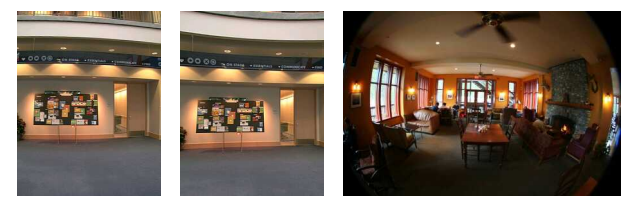
\includegraphics[width=.9\linewidth]{figures/c2/radial_distortion.png}
       \caption[Các loại biến dạng xuyên tâm]{Các loại biến dạng xuyên tâm: (a) barrel, (b) pincushion, và (c) mắt cá. Hình ảnh mắt cá kéo dài gần 180° từ bên này sang bên kia \cite{Szeliski22Book}.}
       \label{fig:radial_distortion}
   \end{center}
\end{figure}

\subsubsection{Biến dạng tiếp tuyến}

Biến dạng tiếp tuyến xảy ra do ống kính và cảm biến ảnh không được căn chỉnh song song hoàn hảo. Nó thường được mô hình hóa bằng hai hệ số $p_1$ và $p_2$. Tọa độ pixel bị biến dạng $(u_d, v_d)$ do biến dạng tiếp tuyến có thể được tính như sau:

\begin{equation}
    \begin{aligned}
x_d &= x + [2 p_1 xy + p_2 (r^2 + 2 x^2)] \\
y_d &= y + [p_1 (r^2 + 2 y^2) + 2 p_2 xy]
\end{aligned}
\end{equation}


\subsubsection{Khử biến dạng}

Mục tiêu của việc khử biến dạng là tìm lại tọa độ pixel không bị biến dạng $(u, v)$ từ tọa độ pixel bị biến dạng $(u_d, v_d)$ và các hệ số biến dạng. Quá trình này thường phức tạp hơn vì các phương trình biến dạng là phi tuyến. Một số phương pháp khử biến dạng bao gồm : 

\begin{itemize}
\item Phương pháp trực tiếp: Cố gắng giải trực tiếp hệ phương trình biến dạng để tìm $(u, v)$ từ $(u_d, v_d)$.
\item Phương pháp lặp: Sử dụng các thuật toán lặp để tìm ra giá trị $(u, v)$ sao cho khi áp dụng mô hình biến dạng, ta thu được giá trị gần đúng với $(u_d, v_d)$ nhất.
\item Sử dụng bản đồ ánh xạ: Tính toán một bản đồ ánh xạ từ tọa độ pixel bị biến dạng sang tọa độ pixel không bị biến dạng và sau đó áp dụng bản đồ này lên ảnh. Đây cũng là cách thư viện OpenCV sử dụng để khử biến dạng bằng việc cung cấp các hàm cv2.undistort và cv2.remap.
\end{itemize}

\section{Phép đạc tam giác}

Phép đạc tam giác (hay triangulation) là một kỹ thuật cơ bản trong thị giác máy tính và tái tạo 3D, được sử dụng để xác định vị trí 3D của một điểm trong không gian dựa trên hình chiếu của nó trên hai hoặc nhiều ảnh được chụp từ các vị trí máy ảnh khác nhau với các tham số máy ảnh đã biết. 

Nguyên lý của phép đạc tam giác dựa trên việc mỗi điểm ảnh trên một bức ảnh tương ứng với một tia sáng trong không gian 3D, xuất phát từ tâm máy ảnh và đi qua điểm ảnh đó. Nếu chúng ta có hai hoặc nhiều ảnh của cùng một điểm 3D, mỗi ảnh sẽ tạo ra một tia sáng tương ứng. Vị trí 3D của điểm đó là giao điểm của các tia sáng này. 

Giả sử chúng ta có hai máy ảnh với ma trận chiếu $\mathbf{P}_1$ và $\mathbf{P}_2$. Một điểm 3D $\mathbf{X} = [X, Y, Z, 1]^T$ được chiếu lên ảnh 1 tại điểm $\mathbf{x}_1 = [u_1, v_1, 1]^T$ và lên ảnh 2 tại điểm $\mathbf{x}_2 = [u_2, v_2, 1]^T$. Theo mô hình máy ảnh pinhole, ta có:


\begin{equation} \label{eq:your_label_here} % Thêm label nếu cần tham chiếu
\begin{aligned}
    s_1 \mathbf{x}_1 &\sim \mathbf{P}_1 \mathbf{X} \\
    s_2 \mathbf{x}_2 &\sim \mathbf{P}_2 \mathbf{X}
\end{aligned}
\end{equation}


Trong đó $s_1$ và $s_2$ là các hệ số tỷ lệ (thường liên quan đến độ sâu của điểm), và $\sim$ biểu thị đẳng thức theo tỷ lệ.

Để tìm $\mathbf{X}$, chúng ta có thể viết lại các phương trình trên thành hệ thống các phương trình tuyến tính. Từ $\mathbf{x}_1 \times (\mathbf{P}_1 \mathbf{X}) = \mathbf{0}$ và $\mathbf{x}_2 \times (\mathbf{P}_2 \mathbf{X}) = \mathbf{0}$, ta thu được một hệ thống các phương trình tuyến tính đồng nhất với ẩn số (X, Y, Z, 1). Chúng ta có thể giải hệ thống này bằng các phương pháp như phân tích giá trị suy biến (hay Singular Value Decomposition - SVD) để tìm ra nghiệm $\mathbf{X}$.   



\section{Tổng quan về tái tạo mô hình mây điểm 3D từ ảnh 2D}
\label{sec:tong_quan_3d}
Trong lĩnh vực xử lý ảnh và thị giác máy tính, bài toán dựng 3D từ ảnh 2D đã và đang trở thành một hướng nghiên cứu quan trọng, với các ứng dụng thực tiễn như dựng mô hình kiến trúc, khảo sát địa hình, và khảo sát các đối tượng kỹ thuật phức tạp như trạm thu phát sóng di động. Quá trình dựng 3D từ ảnh 2D thường được chia thành các giai đoạn chính được mô tả trong Hình \ref{fig:3D_pipeline}, bao gồm: (1) thu thập và tiền xử lý dữ liệu ảnh, (2) trích xuất đặc trưng và khớp nối ảnh, (3) xây dựng đám mây điểm 3D, (4) tái tạo lưới bề mặt, và (5) tạo kết cấu để hoàn thiện mô hình 3D. Trong đó, việc xây dựng đám mây điểm 3D đóng vai trò trung tâm, là bước nền tảng và cũng là bước quan trọng nhất để chuyển từ dữ liệu ảnh 2D sang không gian 3D, cung cấp thông tin về cấu trúc không gian của đối tượng.

\begin{figure}[H]
    \centering
    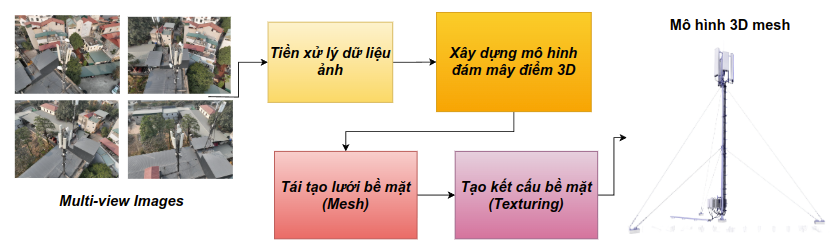
\includegraphics[width=\linewidth]{figures/c2/quy_trinh_3d_from_image.png}
    \caption{Quy trình xây dựng mô hình 3D hoàn chỉnh từ ảnh chụp 2D đa góc nhìn.}
    \label{fig:3D_pipeline}
\end{figure}

Trong phạm vi nghiên cứu của luận văn, luận văn tập trung giải quyết bài toán tái dựng đám mây điểm 3D chi tiết, chính xác cho đối tượng cột ăng-ten. Đám mây điểm 3D không chỉ cung cấp thông tin về hình dạng tổng thể của cột ăng-ten mà còn hỗ trợ phân tích thông tin kĩ thuật kết cấu của cột, cũng như hỗ trợ nhận diện, kiểm đếm, đo đạc các thông số kỹ thuật của các thiết bị được lắp đặt trên cột. Đặc biệt, trong các ứng dụng thực tiễn, đám mây điểm 3D cũng có thể được sử dụng để kiểm tra độ chính xác của thiết kế, phát hiện hư hỏng, hoặc lập kế hoạch bảo trì mà không nhất thiết phải dựng mô hình 3D hoàn chỉnh. Tuy nhiên, do cột BTS thường có cấu trúc phức tạp, bề mặt thiết bị trơn nhẵn, đồng màu nên việc tạo đám mây điểm 3D chi tiết, chính xác cho cột viễn thông là một thách thức lớn.

\subsection{Giới thiệu bài toán tái tạo mô hình đám mây điểm 3D từ ảnh 2D}
\label{subsec:gioi_thieu_bai_toan}
Tái tạo mô hình đám mây điểm 3D từ các hình ảnh 2D là một trong những lĩnh vực nghiên cứu nền tảng và có lịch sử lâu đời trong cả thị giác máy tính và quang trắc học. Đám mây điểm 3D là tập hợp các điểm trong không gian ba chiều, mỗi điểm được xác định bởi tọa độ $(x, y, z)$ và có thể kèm theo thông tin bổ sung như màu sắc. Đầu vào của bài toán là một tập các ảnh 2D đảm bảo một tỉ lệ chồng lấp nhất định giữa các ảnh liền kề nhau trong quỹ đạo chụp. Đầu ra mong muốn là một biểu diễn đám mây điểm 3D của cảnh, phổ biến nhất là dưới dạng một đám mây điểm dày đặc, chi tiết. Quá trình tái tạo đám mây điểm 3D từ ảnh 2D là một bài toán đối mặt với nhiều thách thức. Các thuật toán cần phải đủ mạnh mẽ để đối phó với sự thay đổi về điều kiện chiếu sáng, góc nhìn, sự che khuất, các vùng bề mặt không có hoặc ít đặc trưng thị giác, và các cấu trúc có tính chất lặp lại - những yếu tố thường gặp khi chụp ảnh các cấu trúc công nghiệp như cột ăng-ten viễn thông.

\subsection{Các hướng tiếp cận chính}
\label{subsec:huong_tiep_can}
Trong lĩnh vực thị giác máy tính và quang trắc học, có nhiều phương pháp khác nhau để giải quyết bài toán tái tạo 3D. Luận văn này tập trung vào các phương pháp chỉ sử dụng ảnh 2D thu được từ máy ảnh. Hiện nay, có hai hướng tiếp cận chính, phổ biến trong lĩnh vực này: phương pháp truyền thống dựa trên hình học và phương pháp hiện đại dựa trên Học sâu.

\textbf{Phương pháp truyền thống dựa trên hình học:} Đây là hướng tiếp cận đã được phát triển và hoàn thiện trong nhiều thập kỷ, thường bao gồm hai giai đoạn chính:
\begin{itemize}
    \item Phục dựng cấu trúc từ chuyển động: Giai đoạn này tập trung vào việc ước lượng đồng thời các tham số nội tại, camera pose cho từng ảnh chụp, cũng như cấu trúc hình học của cảnh dưới dạng một tập hợp các điểm 3D thưa thớt. Nền tảng của SfM dựa trên việc phát hiện, mô tả và khớp nối các điểm đặc trưng giữa các ảnh, sau đó sử dụng các ràng buộc hình học đa góc nhìn và tối ưu hóa để đạt được kết quả chính xác \cite{Schonberger16SFMRevisited}. 
    \item Tái tạo lập thể đa góc nhìn: Sau khi đã có được camera pose và cấu trúc thưa từ SfM, MVS được sử dụng để tái tạo cấu trúc hình học dày đặc bằng cách ước định độ sâu cho các điểm ảnh trong ảnh dựa trên nguyên tắc tối ưu hóa sự tương đồng quang học giữa điểm ảnh được xét và hình chiếu của điểm 3D tương ứng với độ sâu của điểm ảnh đó khi chiếu lên các bức ảnh ở góc nhìn khác nhau\cite{Seitz2006comparison, Furukawa2015multi}. Kết quả của MVS thường là một đám mây điểm dày đặc hoặc một lưới 3D.
\end{itemize}
Phương pháp SfM kết hợp với MVS này đã chứng minh được sự hiệu quả và độ tin cậy cao, đặc biệt với các cảnh có đặc trưng bề mặt đối tượng và điều kiện chụp ảnh tốt. Các công cụ mã nguồn mở mạnh mẽ như COLMAP, OpenMVS là các công cụ phổ biến, được sử dụng rộng rãi trong cộng đồng nghiên cứu khoa học.

\textbf{Phương pháp hiện đại dựa trên Học sâu}: Sự bùng nổ của các kiến trúc mạng học sâu đã mang lại những thay đổi và cải tiến đáng kể cho bài toán tái tạo đám mây điểm 3D:
\begin{itemize}
    \item Cải thiện phương pháp truyền thống: Học sâu được ứng dụng kết hợp hoặc thay thế cho các bước của phương pháp SfM kết hợp với MVS để nâng cao hiệu năng. Các bộ phát hiện và mô tả đặc trưng dựa trên học sâu như SuperPoint \cite{detone2018superpoint}, DISK \cite{tyszkiewicz2020disk} và các bộ khớp nối đăc trưng mạnh mẽ như SuperGlue \cite{sarlin2020superglue}, LightGlue \cite{lindenberger2023LightGlue} có thể hoạt động hiệu quả hơn các phương pháp truyền thống trong các điều kiện khó khăn như thay đổi ánh sáng, đặc trưng bề mặt đối tượng ít,... Các kỹ thuật dựa trên học sâu cũng được áp dụng để cải thiện các bước trong MVS như các mô hình MVSNet \cite{Yao2018mvsnet}, SAFE-MVS \cite{wei2023safemvs} với mục tiêu giải quyết các nhược điểm của MVS như thời gian tính toán lâu, kém chi tiết khi tái tạo mây điểm cho các bề mặt đối tượng ít đặc trưng.
    \item Biểu diễn ngầm và kết xuất nơ-ron: Một hướng tiếp cận hoàn toàn mới và đột phá là sử dụng mạng nơ-ron để học một biểu diễn 3D ngầm của cảnh trực tiếp từ ảnh 2D và camera pose. Mô hình NeRF \cite{Mildenhall2020NeRF} là phương pháp tiêu biểu nhất cho hướng này. NeRF học một mạng nơ-ron nhằm biểu diễn cho một không gian 3D liên tục, trong đó, ánh xạ mỗi tọa độ 3D và hướng nhìn tại điểm đó vào một trường màu sắc và mật độ. NeRF cho phép kết xuất các ảnh mới từ các góc nhìn tùy ý với chất lượng rất cao. Mặc dù mục tiêu ban đầu của NeRF là kết xuất hình ảnh góc nhìn mới, các phương pháp trích xuất thông tin hình học từ biểu diễn NeRF cũng đang được phát triển mạnh mẽ cho phép NeRF có thể tái tạo một đám mây điểm 3D cho độ chi tiết, chất lượng rất cao. NeRF và các biến thể của nó đặc biệt mạnh trong việc xử lý các hiệu ứng phụ thuộc góc nhìn và các bề mặt phức tạp, ít đặc trưng.
\end{itemize}

Luận văn sẽ đi sâu vào tìm hiểu các thành phần cốt lõi của các thuật toán trong cả phương pháp truyền thống và hiện đại là SfM, MVS và NeRF trong các mục tiếp theo.
\section{Phục dựng cấu trúc từ chuyển động}

SfM là một quy trình nền tảng và quan trọng trong lĩnh vực thị giác máy tính, đóng vai trò then chốt trong việc khôi phục thông tin hình học 3D của một cảnh hoặc đối tượng từ một tập hợp các hình ảnh 2D được chụp từ các góc nhìn khác nhau. Điểm đặc biệt của SfM là khả năng hoạt động hiệu quả ngay cả khi không có thông tin tiên nghiệm về vị trí và hướng của máy ảnh cũng như thứ tự chụp ảnh \cite{Snavely06Photo}. 
Kết quả đầu ra của quy trình SfM thường bao gồm một đám mây điểm 3D thưa biểu diễn cấu trúc hình học của cảnh, tham số nội tại của máy ảnh và đặc biệt là thông tin camera pose chính xác cho từng ảnh đầu vào. Trong phạm vi nghiên cứu luận văn này, SfM có ý nghĩa đặc biệt quan trọng vì nó cung cấp phương pháp để ước lượng camera pose từ tập ảnh 2D ban đầu – thông tin đầu vào thiết yếu cho việc tái tạo mô hình đám mây điểm chi tiết của MVS và việc huấn luyện mô hình tái tạo 3D chi tiết dựa trên học sâu như NeRF sẽ được trình bày ở các phần sau.

Một quy trình SfM điển hình bao gồm nhiều giai đoạn phức tạp, nhưng phổ biến là được phân chia thành 2 giai đoạn chính: Giai đoạn tìm kiếm sự tương ứng và giai đoạn tái tạo 3D \cite{Schonberger16SFMRevisited}, như biểu diễn trong Hình \ref{fig:incre_sfm}.

\begin{figure}[H]
    \centering
    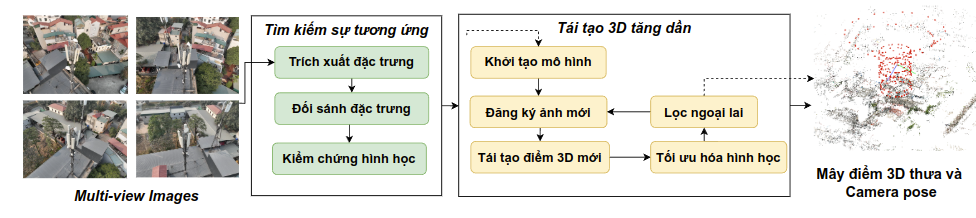
\includegraphics[width=\linewidth]{figures/c3/incremental_sfm.png}
    \caption{Quy trình ước tính camera pose của thuật toán SfM truyền thống.}
    \label{fig:incre_sfm}
\end{figure}

\subsection{Tìm kiếm sự tương ứng}
Mục tiêu của giai đoạn này là phát hiện và xác nhận các điểm ảnh tương ứng trên các ảnh khác nhau trong tập ảnh đầu vào $\mathcal{I} = \{I_i \mid i = 1, \ldots, N_I\}$. Việc xác định đúng các tương ứng này cho phép xây dựng các cặp ảnh có chồng lấp cảnh thực sự và thiết lập các ràng buộc hình học giữa chúng. Các tương ứng được sử dụng để xây dựng một đồ thị quan sát, nơi các đỉnh đại diện cho ảnh và các cạnh đại diện cho mối liên kết hình học giữa các ảnh thông qua các điểm 3D quan sát chung. Độ chính xác của quá trình tìm kiếm tương ứng ảnh hưởng trực tiếp đến chất lượng của việc ước lượng tham số máy ảnh và tái dựng mô hình 3D sau đó. Giai đoạn tìm kiếm sự tương ứng thường bao gồm ba bước chính: (1) Trích xuất đặc trưng, (2) Đối sánh đặc trưng, (3) Kiểm chứng hình học.

\textbf{Trích xuất đặc trưng.} Đối với mỗi ảnh $I_i$, một tập hợp các điểm đặc trưng $\mathcal{F}_{i}=\{(x_{j},f_{j})\}$ được phát hiện tại các vị trí điểm ảnh $x_j = (u, v)$ có cấu trúc đặc trưng nổi bật \cite{McGlone80Manual}. Mỗi điểm đặc trưng này được gắn với một vector mô tả $f_j$ nhằm mã hóa thông tin về vùng ảnh lân cận vị trí đó. Để đảm bảo khả năng đối sánh chính xác giữa các ảnh chụp ở các góc nhìn khác nhau, các đặc trưng và bộ mô tả cần có tính bất biến cao trước các thay đổi về chiếu sáng và phép biến đổi hình học \cite{Tuytelaars08Local}. Ngày nay, các thuật toán trích xuất đặc trưng kinh điển như SIFT \cite{Lowe04Distinctive} và các biến thể của nó, hay gần đây là các đặc trưng được học dựa trên mạng học sâu thường được ưa chuộng và sử dụng trong hầu hết các bài toán vì độ tin cậy và chính xác cao. 

Thuật toán SIFT (Scale-Invariant Feature Transform) là một phương pháp trích xuất đặc trưng hình ảnh được đề xuất bởi David Lowe, được cải tiến vào năm 2004 \cite{Lowe04Distinctive}. SIFT được thiết kế để phát hiện và mô tả các đặc trưng cục bộ trong hình ảnh, đảm bảo tính bất biến đối với thay đổi tỷ lệ, xoay, và một phần đối với thay đổi ánh sáng và góc nhìn. SIFT xây dựng một tháp Gaussian để biểu diễn hình ảnh ở nhiều tỷ lệ khác nhau, từ đó có thể trích xuất ra các điểm đặc trưng có tính bất biến với tỷ lệ. Chính vì vậy các đặc trưng cố định, góc cạnh thường được SIFT ưu tiên trích xuất, minh họa ở Hình \ref{fig:sift_detection}.

\begin{figure}[H]
    \centering
    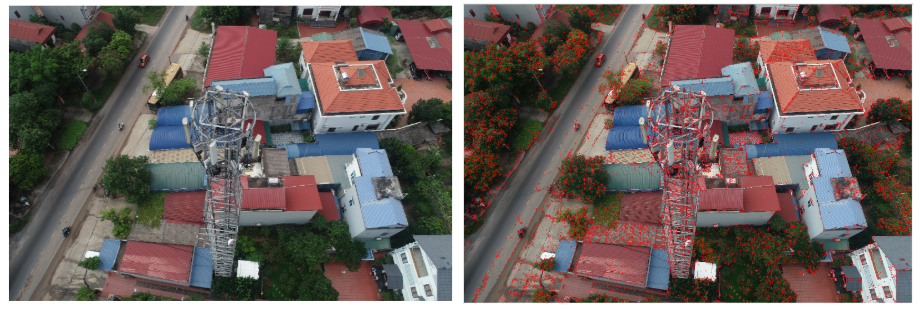
\includegraphics[width=0.9\linewidth]{figures/c2/sift_detection.png}
    \caption{Trích xuất điểm đặc trưng dựa trên SIFT. Các điểm màu đỏ thể hiện điểm đặc trưng quan trọng được phát hiện bởi SIFT. }
    \label{fig:sift_detection}
\end{figure}

\textbf{Đối sánh đặc trưng}. Sau khi phát hiện các đặc trưng của mỗi bức ảnh, bước đối sánh đặc trưng được thực hiện để tìm kiếm các cặp ảnh có khả năng quan sát cùng một điểm trong không gian 3D. Cách tiếp cận đơn giản nhất là duyệt qua tất cả các cặp ảnh và tìm kiếm các cặp đặc trưng có vector mô tả $f_j$ tương đồng nhất giữa chúng. Tuy nhiên, với độ phức tạp tính toán lên tới $O(N_{I}^{2}N_{F_{i}}^{2})$, phương pháp này không khả thi cho các tập ảnh số lượng lớn. Do đó, nhiều kỹ thuật đối sánh hiệu quả và có khả năng mở rộng đã được phát triển để giảm thiểu chi phí tính toán mà vẫn đảm bảo tìm được đủ số lượng đối sánh cần thiết. Kết quả của bước này là một tập hợp các cặp ảnh được khớp nối tiềm năng $\mathcal{C}$ và các cặp đối sánh đặc trưng thô $\mathcal{M}_{ab}$ giữa chúng.

\textbf{Kiểm chứng hình học}. Do việc đối sánh đặc trưng chủ yếu dựa trên sự tương đồng về đặc trưng ngoại hình, tập hợp các đối sánh thô $\mathcal{M}_{ab}$ thường chứa một tỷ lệ đáng kể các cặp sai, gây ảnh hưởng tiêu cực đến kết quả của các bước xử lý sau. Vì vậy, bước kiểm chứng hình học đóng vai trò quan trọng trong việc loại bỏ các đối sánh sai này. Quá trình kiểm chứng được thực hiện bằng cách ước lượng một mô hình biến đổi hình học giữa hai ảnh, nhằm kiểm tra tính nhất quán hình học của các cặp đối sánh thô. Các mô hình thường được sử dụng bao gồm: ma trận homography ($\mathbf{H}$), áp dụng cho trường hợp cảnh phẳng hoặc chuyển động quay; ma trận cơ bản ($\mathbf{F}$) dùng khi các tham số nội tại của máy ảnh chưa được biết; và ma trận cốt yếu ($\mathbf{E}$), sử dụng khi máy ảnh đã được hiệu chuẩn đầy đủ.\cite{Hartley03Multiple}. Vì dữ liệu có chứa ngoại lai, cho nên các phương pháp ước lượng mạnh mẽ như RANSAC \cite{Fischler81RANSAC} hoặc các biến thể của nó được sử dụng để tìm ra mô hình phù hợp nhất được với đa số các đối sánh. Nếu một mô hình hợp lệ được tìm thấy với số lượng cặp đối sánh chính xác đủ lớn, cặp ảnh đó được xem là đã được kiểm chứng hình học, ký hiệu là $\overline{\mathcal{C}}$, và chỉ các đối sánh tốt, ký hiệu là $\overline{\mathcal{M}}_{ab}$ được giữ lại để phục vụ cho các bước tính toán của giai đoạn sau.

Kết thúc giai đoạn tìm kiếm tương ứng, chúng ta thu được đồ thị cảnh với các liên kết hình học đáng tin cậy, làm đầu vào vững chắc cho giai đoạn tái tạo 3D tăng dần sẽ được mô tả ở các phần tiếp theo.

\subsection{Tái tạo tăng dần} 
\label{subsec:incremental_reconstruction} 
    
Quá trình tái tạo cấu trúc 3D thưa trong SfM thường được thực hiện theo ba kiểu quy trình vòng lặp chính bao gồm: quy trình tái tạo tăng dần, quy trình tái tạo toàn cục, quy trình tái tạo kết hợp. Mỗi loại có những ưu, nhược điểm và ứng dụng khác nhau. Trong luận văn này sẽ tập trung giới thiệu về quy trình tái tạo tăng dần, được minh họa trong Hình \ref{fig:incre_sfm}. Đây là một quy trình có tính ổn định cao được sử dụng trong nền tảng COLMAP - một nền tảng mã nguồn mở mạnh mẽ được sử dụng rộng rãi trong lĩnh vực tái tạo 3D.

Sau khi giai đoạn Tìm kiếm sự tương ứng đã thiết lập được đồ thị cảnh với các liên kết hình học đáng tin cậy giữa các cặp ảnh đa góc nhìn, giai đoạn Tái tạo tăng dần bắt đầu được thực hiện để tái tạo thông tin về cấu trúc 3D của cảnh, đối tượng. Mục tiêu của giai đoạn này là xây dựng mô hình hình học 3D của cảnh và ước lượng camera pose một cách tuần tự theo từng vòng lăp. Thuật toán khởi đầu từ một cấu hình nhỏ, có thể là tìm kiếm cặp ảnh có đối sánh cao nhất và dần dần mở rộng bằng cách thêm vào các hình ảnh và điểm 3D mới. Đầu vào chính là đồ thị cảnh đã được kiểm chứng hình học, và đầu ra là một tập hợp các camera pose đã được tối ưu, hiệu chỉnh  $\mathcal{P} = \{P_c \in SE(3)\}$ và một tập hợp các điểm 3D tái tạo $\mathcal{X} = \{X_k \in \mathbb{R}^3\}$ với độ chính xác nhất định dựa trên ngưỡng của chỉ số RE (sai số chiếu lại). Quy trình tái tạo cấu trúc 3D tăng dần bao gồm 2 bước chính: Khởi tạo mô hình và Vòng lặp tái tạo.

\subsubsection{Khởi tạo mô hình }
Quá trình tái tạo tăng dần thường được khởi tạo từ một mô hình hai góc nhìn được lựa chọn cẩn thận từ đồ thị cảnh. Việc chọn cặp ảnh $(I_a, I_b)$ phù hợp để khởi tạo là cực kỳ quan trọng, bởi vì một lựa chọn không tốt ví dụ như đường cơ sở quá ngắn (đường thẳng nối 2 vị trí chụp ảnh), cấu hình hình học suy biến, hoặc ước lượng ma trận F/E không chính xác đều có thể dẫn đến mô hình bị lỗi hoặc không thể phục hồi trong các bước tiếp theo. Các tiêu chí lựa chọn thường bao gồm số lượng đối sánh đặc trưng đủ lớn, các điểm ảnh được phân bố tốt trên cả hai ảnh, và một đường cơ sở phù hợp để đảm bảo phép giao hội đáng tin cậy \cite{Beder06Determining, Snavely08Thesis}.

Vị trí của cặp ảnh khởi tạo trong đồ thị cảnh cũng ảnh hưởng đến chất lượng và hiệu năng của toàn bộ quá trình tái tạo. Khởi tạo từ một vùng dày đặc các ảnh chồng lấn thường mang lại độ chính xác ban đầu cao hơn do có nhiều ràng buộc dư thừa, nhưng cũng có thể làm tăng chi phí tính toán cho các bước tối ưu hóa sau này do mô hình được mở rộng nhanh chóng. Ngược lại, khởi tạo từ vùng thưa hơn có thể giúp giảm thời gian chạy ban đầu nhưng tiềm ẩn rủi ro về độ ổn định của mô hình. Sau khi chọn cặp ảnh khởi tạo, ma trận F hoặc E được phân tích để tìm vị trí, hướng tương đối giữa hai máy ảnh, và các điểm 3D ban đầu được tạo ra bằng phép giao hội từ các đối sánh đặc trưng giữa chúng.

\subsubsection{Vòng lặp tái tạo tăng dần}
Khi mô hình 3D ban đầu đã được thiết lập (bao gồm vị trí, hướng của ít nhất hai máy ảnh và một tập các điểm 3D $\mathcal{X}$), quy trình tái tạo sẽ đi vào một vòng lặp để dần dần mở rộng mô hình bằng cách thêm các ảnh mới. Vòng lặp này thường bao gồm các bước chính sau:

\begin{itemize}
    \item \textbf{Lựa chọn ảnh tiếp theo:} Từ tập các ảnh chưa được liên kết, kiểm tra, hệ thống sẽ lựa chọn một hoặc một vài ảnh "tốt nhất" để thêm vào mô hình ở bước tiếp theo. Tiêu chí lựa chọn rất quan trọng để đảm bảo sự ổn định và chính xác của quá trình tái tạo. Một chiến lược phổ biến là chọn ảnh quan sát được nhiều điểm 3D đã có trong mô hình nhất, vì điều này ảnh hưởng trực tiếp tới độ chính khi xác ước lượng camera pose của ảnh được thêm vào. Các chiến lược phức tạp hơn có thể xem xét cả sự phân bố của các điểm 3D trên ảnh (để tránh các cấu hình PnP suy biến) \cite{Lepetit09EPnP}. Bài báo \cite{Schonberger16SFMRevisited} đề xuất một phương pháp lựa chọn hiệu quả dựa trên việc phân tích đồng thời số lượng và sự phân bố của các điểm 3D nhìn thấy được, cho mỗi ảnh xét duyệt. Việc vừa đảm bảo số lượng điểm 3D quan sát được và phân bố đều trên ảnh sẽ đem lại kết quả tốt hơn cho mô hình.

    \item \textbf{Đăng ký ảnh:} Quá trình đăng ký ảnh đóng vai trò then chốt trong việc mở rộng mô hình 3D từng bước một cách ổn định và chính xác. Bước này nhằm mục tiêu ước lượng camera pose $P_c$ của ảnh mới khi thêm ảnh đó vào mô hình đã có, thông qua việc tận dụng các điểm 3D được tái dựng trước đó và các phép chiếu 2D tương ứng trên ảnh mới.

    Giả sử tại thời điểm hiện tại, hệ thống đã xây dựng được một mô hình 3D tạm thời với tập các điểm 3D \( \mathcal{X} = \{ \mathbf{X}_i \in \mathbb{R}^3 \} \), được quan sát bởi một tập con ảnh đã được đăng ký \( \mathcal{I}_{reg} \subseteq \mathcal{I} \). Với một ảnh mới \( I_{\text{c}} \in \mathcal{I} \setminus \mathcal{I}_{reg} \), mục tiêu của bước đăng ký là tìm "\textit{pose}" của máy ảnh tương ứng với ảnh \( I_{\text{c}} \), biểu diễn dưới dạng ma trận chuyển đổi \( [R \mid \mathbf{t}] \in SE(3) \), trong đó \( R \in SO(3) \) là ma trận xoay và \( \mathbf{t} \in \mathbb{R}^3 \) là vector tịnh tiến.
    
    Để thực hiện điều này, đầu tiên ta tìm kiếm các cặp đối sánh đặc trưng giữa ảnh mới \( I_{\text{c}} \) và các ảnh đã được đăng ký, từ đó ánh xạ đến các điểm 3D đã biết trong mô hình. Kết quả thu được là một tập hợp các cặp tương ứng 2D-3D \( \{ (\mathbf{x}_i, \mathbf{X}_i) \} \), trong đó \( \mathbf{x}_i \in \mathbb{R}^2 \) là vị trí điểm ảnh trong \( I_{\text{c}} \), và \( \mathbf{X}_i \in \mathbb{R}^3 \) là điểm 3D tương ứng đã biết.
    
    Với các cặp tương ứng này, bài toán trở thành một trường hợp cổ điển của bài toán \textit{Perspective-$n$-Point (PnP)}, trong đó ta tìm ma trận \( [R \mid \mathbf{t}] \) sao cho:
    
    \begin{equation}
        \mathbf{x}_i \sim \pi\left( K [R \mid \mathbf{t}] \mathbf{X}_i \right)     
    \end{equation}
    
    trong đó \( K \in \mathbb{R}^{3 \times 3} \) là ma trận thông số nội tại của máy ảnh, và \( \pi(\cdot) \) là phép chiếu từ không gian 3D về mặt phẳng ảnh 2D theo mô hình pinhole.
    
    Để tăng độ bền vững trước nhiễu và các đối sánh sai lệch, việc giải bài toán PnP thường đi kèm với thuật toán \textit{RANSAC}, nhằm loại bỏ các ngoại lai và chỉ giữ lại các cặp đối sánh hình học nhất quán. Khi camera pose ảnh được xác định chính xác, ảnh \( I_{\text{c}} \) sẽ được thêm vào mô hình, trở thành một ảnh đã đăng ký.
    
    \item \textbf{Tạo điểm 3D mới - Phép giao hội:} tạo các điểm 3D mới từ các cặp đối sánh giữa ảnh mới \( I_{\text{c}} \) và các ảnh đã được đăng ký trước đó. Quá trình này được gọi là phép giao hội, bởi nó tìm tọa độ không gian của điểm 3D từ hai hoặc nhiều phép chiếu 2D của điểm đó trên các mặt phẳng ảnh của các ảnh khác nhau.

    Cụ thể, giả sử điểm ảnh \( \mathbf{x}_i^{(1)} \in \mathbb{R}^2 \) trong ảnh \( I_1 \) và điểm ảnh tương ứng \( \mathbf{x}_i^{(2)} \in \mathbb{R}^2 \) trong ảnh \( I_2 \) là các hình chiếu của cùng một điểm 3D \( \mathbf{X}_i \in \mathbb{R}^3 \). Biết được ma trận nội tại \( K \) và ma trận tham số trận ngoại (camera pose) \( [R_1\mid\mathbf{t}_1] \), \( [R_2\mid\mathbf{t}_2] \) của hai máy ảnh tương ứng, ta có thể xây dựng phương trình chiếu:
    \begin{align}
        \lambda_1 \mathbf{x}_i^{(1)} &= K \left[ R_1 \mid \mathbf{t}_1 \right] \mathbf{X}_i \\
        \lambda_2 \mathbf{x}_i^{(2)} &= K \left[ R_2 \mid \mathbf{t}_2 \right] \mathbf{X}_i
    \end{align}
    
    trong đó \( \lambda_1 \), \( \lambda_2 \) là các hệ số tỷ lệ liên quan đến độ sâu. Từ hai phương trình trên, ta có thể xây dựng hệ phương trình tuyến tính hoặc phi tuyến để giải cho tọa độ \( \mathbf{X}_i \). Trong thực tế, vì tồn tại nhiễu trong dữ liệu và sai số nội tại trong phép chiếu, các tia chiếu từ ảnh không cắt nhau chính xác mà thường là chéo nhau trong không gian. Do đó, điểm 3D \( \mathbf{X}_i \) được ước lượng là điểm gần nhất tới hai đường thẳng chiếu, hay còn gọi là điểm tối thiểu hóa khoảng cách tới hai tia.
    
    Một cách tiếp cận phổ biến là sử dụng phương pháp giao hội tuyến tính, dựa trên việc xây dựng ma trận \( A \) từ các phương trình chiếu và giải hệ:
    
    \begin{equation}
        A \mathbf{X}_i = 0    
    \end{equation}
    
    sử dụng thuật toán phân tích trị riêng. Ngoài ra, cũng có thể áp dụng giao hội phi tuyến để tối ưu hóa trực tiếp sai số RE:
    
    \begin{equation}
        \mathbf{RE} = \sum_{j=1}^{n} \left\| \mathbf{x}_i^{(j)} - \pi\left( K [R_j \mid \mathbf{t}_j] \mathbf{X}_i \right) \right\|^2    
    \end{equation}    
    trong đó \( \mathbf{x}_i^{(j)} \) là tọa độ điểm ảnh quan sát điểm 3D \( \mathbf{X}_i \) từ máy ảnh thứ \( j \), và \( \pi(\cdot) \) là hàm chiếu pinhole.
    
    Tuy nhiên, không phải mọi cặp đối sánh đều được sử dụng để giao hội. Để đảm bảo độ chính xác và ổn định, chỉ những đối sánh có góc cơ sở đủ lớn và sai số chiếu lại thấp mới được lựa chọn. Góc cơ sở quá nhỏ dẫn đến giao hội yếu và điểm 3D kém chính xác. Ngoài ra, các điểm có số lần quan sát từ nhiều ảnh khác nhau thường được ưu tiên vì giúp cải thiện độ tin cậy của ước lượng tọa độ.
    
    Kết quả của bước này là mở rộng tập điểm 3D \( \mathcal{X} \) trong mô hình hiện tại bằng cách thêm vào các điểm mới \( \mathbf{X}_i \) được tái dựng từ ảnh mới vừa được đăng ký. Những điểm mới này sẽ tiếp tục được sử dụng trong các bước sau và việc đăng ký các ảnh tiếp theo.

    
    \item \textbf{Tối ưu hóa hình học :} Sau khi các điểm 3D mới được tạo ra thông qua phép giao hội, bước quan trọng tiếp theo là tinh chỉnh toàn bộ mô hình để giảm thiểu sai số RE, và đảm bảo sự nhất quán toàn cục của cả cấu trúc không gian 3D và thông số máy ảnh. Quá trình này được gọi là Tối ưu hóa hình học (BA), và được xem là bước cốt lõi trong các hệ thống SfM. Mục tiêu của Tối ưu hóa hình học (BA)\cite{Triggs00Bundle} là đồng thời tối ưu cả các thông số camera pose \( \{ \mathbf{R}_j, \mathbf{t}_j \} \) của mỗi ảnh \( I_{\text{j}} \), các thông số nội tại (nếu cần) và toạ độ không gian của các điểm 3D \( \{ \mathbf{X}_i \} \), sao cho sai số chiếu lại RE là nhỏ nhất. Với một tập các quan sát 2D \( \mathbf{x}_{ij} \) là ảnh chiếu của điểm 3D \( \mathbf{X}_i \) lên ảnh \( I_{\text{j}} \), bài toán được mô hình hoá thành một bài toán tối ưu phi tuyến:

    \begin{equation}
        \min_{\{ \mathbf{R}_j, \mathbf{t}_j, \mathbf{X}_i \}} \sum_{i,j} \rho\left( \left\| \mathbf{x}_{ij} - \pi\left(K_j [\mathbf{R}_j \mid \mathbf{t}_j] \mathbf{X}_i \right) \right\|^2 \right)    
    \end{equation}
    
    Trong đó:
    \begin{itemize}
        \item \( \pi(\cdot) \): hàm chiếu từ không gian 3D về mặt phẳng ảnh,
        \item \( K_j \): ma trận nội tại của máy ảnh thứ \( j \),
        \item \( \rho(\cdot) \): hàm mất mát, ví dụ hàm Huber để giảm ảnh hưởng của nhiễu và ngoại lai,
        \item \( \| \cdot \| \): chuẩn Euclid thể hiện độ lệch giữa điểm ảnh thực tế và điểm ảnh được chiếu lại từ mô hình.
    \end{itemize}
    
    Quá trình tối ưu này thường sử dụng các thuật toán như Levenberg–Marquardt hoặc Gauss–Newton để giải bài toán phi tuyến với số lượng biến lớn. Nhờ tính chất thưa của bài toán (mỗi điểm 3D chỉ được quan sát bởi một vài máy ảnh), một vài kỹ thuật tối ưu hóa hiệu quả nhằm đơn giản hóa bài toán như sử dụng phân rã Schur \cite{triggs1999bundle} giúp rút gọn số lượng biến cần giải, chỉ tập trung vào phần liên quan đến thông số camera pose.
    
    Trong hệ thống SfM sử dụng chiến lược tái tạo tăng dần, việc thực hiện BA toàn cục sau mỗi lần thêm ảnh là không khả thi do chi phí tính toán cao. Thay vào đó, hệ thống áp dụng BA cục bộ, chỉ tối ưu tập con bao gồm máy ảnh mới được thêm vào và các máy ảnh lân cận có quan sát chung với một tập điểm 3D. Phương pháp này cho phép duy trì hiệu quả tính toán trong khi vẫn đảm bảo độ chính xác hình học của mô hình được xây dựng.
    
    Tóm lại, BA đóng vai trò then chốt trong việc nâng cao độ chính xác của mô hình 3D bằng cách giảm thiểu sai số chiếu lại tổng thể của cả mô hình, đồng thời đảm bảo tính nhất quán giữa các quan sát 2D và cấu trúc không gian 3D tái dựng.
    \item \textbf{Lọc ngoại lai:} Sau các bước trên, đặc biệt là sau quá trình Bundle Adjustment, thuật toán sẽ thực hiện lọc bỏ các điểm 3D không đáng tin cậy. Cụ thể, các điểm có lỗi chiếu lại lớn, không thỏa mãn ràng buộc hình học, hoặc được tạo ra từ phép giao hội với góc nhìn quá hẹp sẽ bị loại bỏ \cite{Snavely08Thesis, Wu13Towards}. Việc này giúp loại bỏ các ước lượng sai lệc, cải thiện chất lượng và độ tin cậy của mô hình.
\end{itemize}

Vòng lặp trên được lặp lại cho đến khi không còn ảnh nào có thể được đăng ký một cách đáng tin cậy hoặc khi đạt được một tiêu chí dừng khác. Kết quả cuối cùng là một mô hình 3D thưa và tập hợp các camera pose đã được tối ưu hóa.

% \section{Thuật toán trích xuất đặc trưng SIFT} \label{subsec:sift}

Thuật toán SIFT (Scale-Invariant Feature Transform) là một phương pháp trích xuất đặc trưng hình ảnh được đề xuất bởi David Lowe vào năm 1999, được cải tiến vào năm 2004 \cite{Lowe04Distinctive}. SIFT được thiết kế để phát hiện và mô tả các đặc trưng cục bộ trong hình ảnh, đảm bảo tính bất biến đối với thay đổi tỷ lệ, xoay, và một phần đối với thay đổi ánh sáng và góc nhìn. Các đặc trưng SIFT được sử dụng rộng rãi trong các bài toán trong thị giác máy tính như ghép ảnh, nhận diện đối tượng, và tái tạo cấu trúc 3D từ chuyển động.

\subsection{Xây dựng tháp Gaussian và phát hiện cực trị}

Bước đầu tiên của SIFT là xây dựng một tháp Gaussian để biểu diễn hình ảnh ở nhiều tỷ lệ khác nhau, từ đó đảm bảo tính bất biến tỷ lệ. Hình ảnh đầu vào $I(x, y)$ được làm mờ dần bằng phép tích chập với hàm Gaussian:

\begin{equation}
L(x, y, \sigma) = G(x, y, \sigma) * I(x, y),
\end{equation}
trong đó $G(x, y, \sigma)$ là hàm Gaussian 2D được định nghĩa như sau:

\begin{equation}
G(x, y, \sigma) = \frac{1}{2\pi\sigma^2} e^{-\frac{x^2 + y^2}{2\sigma^2}}.
\end{equation}

\begin{figure}[H]
    \centering
    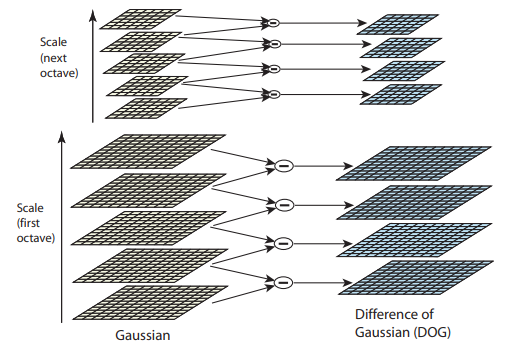
\includegraphics[width=0.6\linewidth]{figures/c3/Hình 1 paper sift.png}
    \caption{Tạo không gian Hiệu số Gauss từ các tầng ảnh khác nhau \cite[Fig.~1]{Lowe04Distinctive}.}
    \label{fig:dog}
\end{figure}

Hàm $L(x, y, \sigma)$ biểu diễn hình ảnh ở mức độ làm mờ với tham số tỷ lệ $\sigma$. Tháp Gaussian được xây dựng bằng cách tăng dần $\sigma$ trong mỗi tầng của tháp và giảm kích thước hình ảnh ở các tầng cao hơn để giảm chi phí tính toán. Để phát hiện các điểm đặc trưng bất biến tỷ lệ, SIFT sử dụng không gian Hiệu số Gauss (DoG) - mô tả tại Hình \ref{fig:dog}, được tạo nên bằng cách tính bằng hiệu của hai hình ảnh làm mờ ở các mức độ $\sigma$ khác nhau trong cùng 1 tầng:

\begin{equation}
D(x, y, \sigma) = L(x, y, k\sigma) - L(x, y, \sigma),
\end{equation}
với $k$ là hằng số nhân tỷ lệ (thường $k = 2^{1/s}$, $s$ là số mức trong một tầng). Hàm $D(x, y, \sigma)$ gần đúng với Laplacian của Gaussian, giúp phát hiện các vùng có sự thay đổi cường độ đáng kể, tương ứng với các đặc trưng tiềm năng.

\begin{figure}[H]
    \centering
    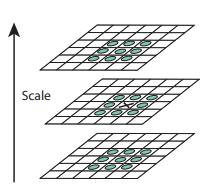
\includegraphics[width=0.4\linewidth]{figures/c3/so_sanh_x_vs_26p_Hinh_2_sift.png}
    \caption{Mô tả vùng lân cận của điểm X được sử dụng để tìm cực trị\cite[Fig.~2]{Lowe04Distinctive}.}
    \label{fig:lan_can_x}
\end{figure}

Các điểm cực trị trong không gian DoG được xác định bằng cách so sánh mỗi điểm trong hình ảnh DoG với các điểm lân cận của nó trong không gian 3D được mô tả trong Hình \ref{fig:lan_can_x} . Giả sử bạn đang xét điểm $(x, y, \sigma_i)$ trong hình ảnh DoG tại mức làm mờ $\sigma_i$. Vùng lân cận 3D có thể được mô tả như một khối 3x3x3 (3 điểm ảnh theo $x$, 3 điểm ảnh theo $y$, 3 mức tỷ lệ mờ lần lượt là $\sigma_{i-1}$, $\sigma$, $\sigma_{i11}$), với điểm đang xét nằm ở trung tâm (Các hình ảnh DoG này nằm trên cùng 1 tầng kích thước). Tổng số điểm trong khối này là $3 \times 3 \times 3 = 27$, do đó, mỗi điểm sẽ so sánh giá trị với 26 điểm lân cận còn lại.
Một điểm được coi là cực trị nếu nó có giá trị lớn nhất hoặc nhỏ nhất trong vùng lân cận đó. Những điểm này là ứng viên cho các điểm đặc trưng. 

\subsection{Tinh chỉnh vị trí điểm đặc trưng}

Sau khi xác định các điểm cực trị, SIFT tinh chỉnh vị trí và loại bỏ các điểm không ổn định. Vị trí chính xác của điểm đặc trưng được xác định bằng cách sử dụng xấp xỉ Taylor bậc hai của hàm $D(x, y, \sigma)$ quanh điểm cực trị:

\begin{equation}
D(\mathbf{x}) = D + \frac{\partial D}{\partial \mathbf{x}}^T \mathbf{x} + \frac{1}{2} \mathbf{x}^T \frac{\partial^2 D}{\partial \mathbf{x}^2} \mathbf{x},
\end{equation}
trong đó $\mathbf{x} = (x, y, \sigma)^T$ là vector vị trí và tỷ lệ. Điểm cực trị được tìm bằng cách lấy đạo hàm và đặt bằng 0:

\begin{equation}
\hat{\mathbf{x}} = -\left( \frac{\partial^2 D}{\partial \mathbf{x}^2} \right)^{-1} \frac{\partial D}{\partial \mathbf{x}}.
\end{equation}

Nếu giá trị $|\hat{\mathbf{x}}|$ quá lớn (vượt ngưỡng, ví dụ 0.5 theo đơn vị pixel), điểm cực trị được coi là không ổn định và bị loại bỏ. Ngoài ra, các điểm có độ tương phản thấp (giá trị $|D(\hat{\mathbf{x}})|$ nhỏ) hoặc nằm trên cạnh cũng bị loại bỏ để đảm bảo tính ổn định.

\subsection{Gán hướng cho điểm đặc trưng}

Để đảm bảo tính bất biến xoay, mỗi điểm đặc trưng được gán một hướng chính dựa trên gradient của hình ảnh xung quanh. Gradient tại điểm $(x, y)$ trong hình ảnh $L(x, y, \sigma)$ được tính như sau:

\begin{equation}
m(x, y) = \sqrt{\left( L(x+1, y) - L(x-1, y) \right)^2 + \left( L(x, y+1) - L(x, y-1) \right)^2},
\end{equation}

\begin{equation}
\theta(x, y) = \tan^{-1} \left( \frac{L(x, y+1) - L(x, y-1)}{L(x+1, y) - L(x-1, y)} \right).
\end{equation}

Trong đó, $m(x, y)$ là độ lớn gradient và $\theta(x, y)$ là hướng gradient. Các hướng gradient trong một vùng xung quanh điểm đặc trưng được tổng hợp thành một histogram hướng. Đỉnh cao nhất trong histogram được chọn làm hướng chính, và các đỉnh phụ (nếu vượt 80\% giá trị đỉnh chính \cite{Lowe04Distinctive}) cũng có thể được sử dụng để tạo thêm điểm đặc trưng, tăng tính mạnh mẽ.

\subsection{Mô tả đặc trưng SIFT}

Cuối cùng, SIFT tạo ra một vector mô tả đặc trưng cho mỗi điểm đặc trưng, đảm bảo tính bất biến với thay đổi tỷ lệ, xoay và ánh sáng. Một vùng xung quanh điểm đặc trưng (kích thước tỷ lệ với $\sigma$) được chia thành lưới 4x4 ô. Trong mỗi ô, gradient được tổng hợp thành histogram hướng với 8 khoảng giá trị (chia đều 360 độ thành 8 khoảng giá trị). Từ đó, tổng hợp ra vector mô tả cuối cùng là một vector 128 chiều (4x4x8), được chuẩn hóa để loại bỏ ảnh hưởng của thay đổi ánh sáng.

Quá trình chuẩn hóa bao gồm việc chia vector cho độ lớn Euclidean của nó:

\begin{equation}
\mathbf{d} = \frac{\mathbf{d}}{\|\mathbf{d}\|_2},
\end{equation}
trong đó $\mathbf{d}$ là vector mô tả. Để giảm ảnh hưởng của các giá trị gradient lớn, các phần tử trong vector được giới hạn (thường ở mức 0.2) và vector được chuẩn hóa lại.

\subsection{Ý nghĩa của SIFT}

SIFT nổi bật nhờ khả năng tạo ra các đặc trưng cục bộ mạnh mẽ, bất biến với các biến đổi hình học. Những tính chất này làm cho SIFT trở thành một công cụ quan trọng trong các ứng dụng SfM, nơi cần khớp các điểm đặc trưng giữa các hình ảnh có góc nhìn và điều kiện khác nhau.

\section{Các thuật toán trích xuất và so khớp đặc trưng dựa trên học sâu}
\subsection{Thuật toán trích xuất đặc trưng ALIKED} \label{sec:aliked}

Thuật toán ALIKED là một thuật toán trích xuất và mô tả đặc trưng hình ảnh hiện đại, được thiết kế để phát hiện và mô tả các điểm đặc trưng bất biến với các biến đổi hình học như xoay, thay đổi tỷ lệ, và biến đổi affine \citep{zhao2023aliked}. ALIKED nổi bật với khả năng hoạt động hiệu quả trong các ứng dụng thị giác máy tính như ghép ảnh, tái tạo 3D, định vị robot và lập bản đồ. Trong phần này, luận văn sẽ trình bày bản chất ý tưởng, kiến trúc mô hình, các công thức liên quan, cũng như phân tích điểm mạnh và điểm yếu của thuật toán.

\textbf{Bản chất ý tưởng và mô hình}. ALIKED được phát triển dựa trên sự kết hợp giữa học sâu và các kỹ thuật truyền thống trong trích xuất đặc trưng, nhằm giải quyết các hạn chế của các thuật toán cổ điển như SIFT \citep{Lowe04Distinctive} hay ORB \citep{rublee2011orb} trong các điều kiện ánh sáng thay đổi và biến đổi hình học phức tạp. Ý tưởng cốt lõi của ALIKED là sử dụng mạng nơ-ron sâu để đồng thời phát hiện các điểm đặc trưng và tạo ra các mô tả đặc trưng bất biến với các biến đổi affine. 

%%%%% CHÈN ẢNH CHO ALIKED
Kiến trúc mô hình của ALIKED bao gồm ba thành phần chính:
\begin{enumerate}
    \item Mạng phát hiện điểm đặc trưng: Sử dụng kiến trúc dựa trên mạng tích chập để xác định các điểm đặc trưng có tính lặp lại cao trên hình ảnh.
    \item Mạng mô tả đặc trưng: Tạo ra các vector mô tả đặc trưng bất biến với các biến đổi hình học và ánh sáng.
    \item Hàm mất mát tối ưu hóa: Đảm bảo rằng các điểm đặc trưng được phát hiện có tính lặp lại và các mô tả đặc trưng có khả năng phân biệt cao.
\end{enumerate}

Kiến trúc mạng của ALIKED thường dựa trên các lớp tích chập với các bộ lọc học được, kết hợp với các kỹ thuật chuẩn hóa và kích hoạt phi tuyến như ReLU. Mạng được huấn luyện trên các tập dữ liệu lớn như MegaDepth \citep{li2018megadepth} để đảm bảo khả năng tổng quát hóa.

\textbf{Quy trình trích xuất và mô tả đặc trưng}. Quá trình trích xuất đặc trưng trong ALIKED có thể được mô tả thông qua các bước sau:
\begin{itemize}
   \item Phát hiện điểm đặc trưng: Đầu vào là một hình ảnh \( I \in \mathbb{R}^{H \times W \times C} \), trong đó \( H \), \( W \), \( C \) lần lượt là chiều cao, chiều rộng và số kênh màu. Mạng phát hiện điểm đặc trưng ánh xạ hình ảnh thành một bản đồ điểm đặc trưng (gọi là score map) \( S \in \mathbb{R}^{H' \times W'} \), với \( H' \leq H \), \( W' \leq W \). Score map \( S \) biểu thị mức độ "đặc trưng" của mỗi vị trí trên hình ảnh, trong đó giá trị cao hơn tại một điểm \( (x, y) \) cho thấy điểm đó có khả năng cao là một điểm đặc trưng ổn định và lặp lại được qua các biến đổi hình học. Bản đồ này được tính bằng:
   \begin{equation}
       S = f_{\text{det}}(I; \theta_{\text{det}}),
   \end{equation}
   trong đó \( f_{\text{det}} \) là hàm mạng phát hiện với tham số \( \theta_{\text{det}} \). Để chọn các điểm đặc trưng, ALIKED áp dụng kỹ thuật tìm cực đại cục bộ (non-maximum suppression) trên \( S \), đảm bảo chỉ giữ lại các điểm có giá trị \( S(x, y) \) lớn hơn các điểm lân cận trong một cửa sổ lân cận (ví dụ, cửa sổ \( 3 \times 3 \)). Điều này giúp loại bỏ các điểm đặc trưng yếu hoặc không ổn định. Ngoài ra, để tăng tính chính xác, ALIKED có thể sử dụng kỹ thuật nội suy để xác định vị trí điểm đặc trưng ở độ phân giải thấp hơn \( (H', W') \) và ánh xạ ngược về không gian hình ảnh gốc.

   \item  Mô tả đặc trưng: Với mỗi điểm đặc trưng \( p_i = (x_i, y_i) \), mạng mô tả tạo ra một vector mô tả \( d_i \in \mathbb{R}^D \), trong đó \( D \) là chiều của vector mô tả (thường là 128 hoặc 256). Vector mô tả được tính bằng:
   \begin{equation}
       d_i = f_{\text{desc}}(I, p_i; \theta_{\text{desc}}),
   \end{equation}
   trong đó \( f_{\text{desc}} \) là hàm biểu diễn mạng mô tả đặc trưng với tham số \( \theta_{\text{desc}} \).
   \item Hàm mất mát:  ALIKED sử dụng hàm mất mát kết hợp để tối ưu hóa cả phát hiện và mô tả đặc trưng. Hàm mất mát tổng quát có dạng:
   \begin{equation}
       \mathcal{L} = \mathcal{L}_{\text{det}} + \lambda \mathcal{L}_{\text{desc}},
   \end{equation}
   trong đó \( \mathcal{L}_{\text{det}} \) là mất mát cho phát hiện điểm đặc trưng, \( \mathcal{L}_{\text{desc}} \) là mất mát cho mô tả đặc trưng, và \( \lambda \) là trọng số cân bằng hai thành phần này.

   Mục tiêu của mất mát phát hiện đặc trưng (\( \mathcal{L}_{\text{det}} \)) là đảm bảo các điểm đặc trưng được phát hiện có tính lặp lại cao, tức là các điểm này có thể được phát hiện lại trong các hình ảnh liên quan. Ví dụ, hình ảnh có cùng cảnh nhưng được chụp từ các góc nhìn khác nhau. Mất mát phát hiện đặc trưng được thiết kế dựa trên bản đồ điểm đặc trưng \( S \). Một cách tiếp cận phổ biến là sử dụng hàm mất mát dựa trên xác suất softmax để ưu tiên các điểm đặc trưng thực sự:
   \begin{equation}
       \mathcal{L}_{\text{det}} = -\sum_{p_i \in \mathcal{P}} \log \left( \frac{\exp(S(p_i))}{\sum_{p_j \in \mathcal{N}_i} \exp(S(p_j))} \right),
   \end{equation}
   trong đó \( \mathcal{P} \) là tập hợp các điểm đặc trưng thực, và \( \mathcal{N}_i \) là tập hợp các điểm lân cận của \( p_i \) trên score map. Hàm này khuyến khích giá trị \( S(p_i) \) tại các điểm đặc trưng thực cao hơn so với các điểm lân cận, từ đó tăng tính lặp lại và độ chính xác của việc phát hiện. Ngoài ra, để xử lý các trường hợp có ít điểm đặc trưng, ALIKED có thể sử dụng các kỹ thuật cân bằng như focal loss để giảm thiểu ảnh hưởng của các vùng không chứa đặc trưng.

   Mục tiêu của Mất mát mô tả (\( \mathcal{L}_{\text{desc}} \)) là đảm bảo các vector mô tả \( d_i \) có tính phân biệt cao, tức là khoảng cách giữa các vector mô tả của các điểm đặc trưng khớp nhau nhỏ, trong khi khoảng cách với các điểm không khớp lớn. ALIKED sử dụng mất mát triplet:
   \begin{equation}
       \mathcal{L}_{\text{desc}} = \sum_{(d_i, d_j, d_k)} \max \left( 0, \| d_i - d_j \|_2^2 - \| d_i - d_k \|_2^2 + m \right),
   \end{equation}
   trong đó \( (d_i, d_j, d_k) \) là một bộ ba đặc trưng (đặc trưng gốc, đặc trưng khớp, đặc trưng không khớp), \( \| \cdot \|_2^2 \) là bình phương khoảng cách Euclid, và \( m \) là ngưỡng margin (thường được chọn trong khoảng 0.5 đến 1.0). Mất mát triplet đảm bảo rằng khoảng cách giữa \( d_i \) và \( d_j \) nhỏ hơn khoảng cách giữa \( d_i \) và \( d_k \) ít nhất bằng \( m \), từ đó cải thiện khả năng phân biệt của các mô tả đặc trưng. Để tăng hiệu quả huấn luyện, ALIKED thường sử dụng kỹ thuật "Khai thác mẫu âm khó" (hay hard negative mining), tức là lựa chọn các đặc trưng không khớp có khoảng cách gần nhất với đặc trưng gốc để tối ưu hóa.
\end{itemize}

\textbf{Điểm mạnh}

ALIKED có một số điểm mạnh nổi bật:
\begin{itemize}
    \item Bất biến với biến đổi affine: Nhờ sử dụng các kỹ thuật học sâu, ALIKED duy trì hiệu suất cao trong các điều kiện có biến đổi hình học phức tạp \citep{zhao2023aliked}.
    \item Hiệu quả tính toán: So với các phương pháp truyền thống như SIFT, ALIKED có tốc độ xử lý nhanh hơn trên phần cứng hiện đại, đặc biệt khi sử dụng GPU.
    \item Tính lặp lại cao: Các điểm đặc trưng được phát hiện bởi ALIKED có độ lặp lại tốt, ngay cả trong các điều kiện ánh sáng thay đổi hoặc góc nhìn khác nhau.
\end{itemize}

\textbf{Điểm yếu}

Mặc dù có nhiều ưu điểm, ALIKED cũng tồn tại một số hạn chế:
\begin{itemize}
    \item Phụ thuộc vào dữ liệu huấn luyện: Hiệu suất của ALIKED phụ thuộc lớn vào chất lượng và độ đa dạng của tập dữ liệu huấn luyện. Trong các kịch bản chưa được huấn luyện trước, hiệu suất có thể giảm \citep{zhao2023aliked}.
    \item Yêu cầu tài nguyên tính toán cao: Mặc dù nhanh hơn SIFT, ALIKED vẫn đòi hỏi phần cứng mạnh (như GPU) để đạt hiệu suất thời gian thực.
    \item Độ phức tạp mô hình: Kiến trúc mạng sâu của ALIKED có thể khó tối ưu hóa hoặc điều chỉnh cho các ứng dụng cụ thể so với các phương pháp truyền thống đơn giản hơn.
\end{itemize}

ALIKED là một thuật toán trích xuất đặc trưng tiên tiến, kết hợp sức mạnh của học sâu với các yêu cầu về bất biến hình học và ánh sáng trong thị giác máy tính. Mặc dù còn tồn tại một vài hạn chế, ALIKED vẫn rất tiềm năng để ứng dụng cho các bài toán thực tế như bài toán tái tạo mây điểm 3D chi tiết, chính xác cho đối tượng cột ăng-ten.
\subsection{Thuật toán so khớp LightGlue}

Thuật toán LightGlue \cite{lindenberger2023LightGlue} là một mạng nơ-ron sâu được thiết kế để thực hiện việc khớp các đặc trưng cục bộ giữa các cặp ảnh, với mục tiêu cải thiện hiệu quả và độ chính xác so với các phương pháp truyền thống. LightGlue được phát triển dựa trên nền tảng của SuperGlue \cite{sarlin2020superglue} – một mô hình tiên tiến trong lĩnh vực so khớp đặc trưng – LightGlue mang đến những cải tiến đáng kể về hiệu suất tính toán, độ chính xác, và khả năng huấn luyện. Đặc biệt, LightGlue có khả năng thích ứng với độ khó của bài toán, giúp giảm thời gian suy luận trên các cặp ảnh dễ khớp. LightGlue đang được ưa chuộng sử dụng cho nhiều các bài toán thực tế như định vị robot, xây dựng bản đồ, tái tạo 3D,...

\textbf{Bản chất ý tưởng và mô hình}

LightGlue được xây dựng dựa trên kiến trúc Transformer, tận dụng cơ chế tự chú ý và chú ý chéo để tăng cường khả năng khớp đặc trưng. Ý tưởng cốt lõi của LightGlue là tối ưu hóa quá trình khớp đặc trưng bằng cách giảm thiểu các phép tính không cần thiết thông qua hai cơ chế chính:

\begin{itemize}
    \item Dừng sớm: LightGlue sử dụng một bộ phân loại độ tin cậy để đánh giá mức độ tin cậy của các dự đoán tại mỗi tầng của mạng. Nếu dự đoán tại một tầng sớm đạt độ tin cậy cao, quá trình suy luận sẽ dừng lại, giúp tiết kiệm thời gian tính toán.
    \item Cắt tỉa điểm đặc trưng: Các điểm đặc trưng được dự đoán là không thể khớp sẽ bị loại bỏ sớm khỏi quá trình suy luận, giảm số lượng phép tính trong các tầng sau.
\end{itemize}

\begin{figure}[H]
    \centering
    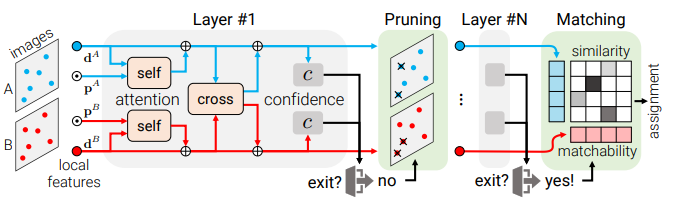
\includegraphics[width=\linewidth]{figures/c3/kien_truc_light_glue.png}
    \caption{Kiến trúc mạng thuật toán so khớp LightGlue \cite[Fig.~3]{lindenberger2023LightGlue}.}
    \label{fig:lightglue}
\end{figure}

Mô hình LightGlue nhận đầu vào là tập hợp các điểm đặc trưng và véc-tơ mô tả đặc trưng tương ứng. Quá trình so khớp được minh họa ở Hình \ref{fig:lightglue} bao gồm các bước sau:

\begin{itemize}
    \item Khởi tạo đặc trưng ban đầu: Các điểm đặc trưng từ hai ảnh được biểu diễn dưới dạng tập hợp $\mathcal{F}_0 = \{(\mathbf{k}_i^0, \mathbf{d}_i^0)\}_{i=1}^{N_0}$ và $\mathcal{F}_1 = \{(\mathbf{k}_j^1, \mathbf{d}_j^1)\}_{j=1}^{N_1}$, trong đó $\mathbf{k}_i^0, \mathbf{k}_j^1 \in \mathbb{R}^2$ là tọa độ điểm đặc trưng, và $\mathbf{d}_i^0, \mathbf{d}_j^1 \in \mathbb{R}^D$ là các vector mô tả đặc trưng. Tại bước này, các vector mô tả đặc trưng được mã hóa thêm thông tin vị trí để tăng cường khả năng biểu diễn không gian:
    \begin{equation}
        \mathbf{x}_i^0 = \mathbf{d}_i^0 + \text{PE}(\mathbf{k}_i^0), \quad \mathbf{x}_j^1 = \mathbf{d}_j^1 + \text{PE}(\mathbf{k}_j^1),
    \end{equation}
    trong đó $\text{PE}(\cdot)$ là hàm mã hóa vị trí.

    \item Tăng cường ngữ cảnh qua tự chú ý: 
    Mỗi tập đặc trưng $\mathcal{F}_0$ và $\mathcal{F}_1$ được xử lý độc lập thông qua các tầng tự chú ý trong Transformer để tích hợp thông tin ngữ cảnh cục bộ từ các điểm đặc trưng lân cận trong cùng một ảnh. Quá trình này được biểu diễn như sau:
    \begin{equation}
        \mathbf{x}_i^{0'} = \text{SelfAttention}(\mathbf{x}_i^0, \{\mathbf{x}_k^0\}_{k=1}^{N_0}; \theta_s),
    \end{equation}
    trong đó $\theta_s$ là tham số của mô-đun tự chú ý. Tương tự cho $\mathcal{F}_1$. Bước này giúp các đặc trưng trở nên phong phú hơn bằng cách học mối quan hệ giữa các điểm trong cùng một ảnh.

    \item Tích hợp thông tin qua chú ý chéo: 
    Sau khi tăng cường ngữ cảnh cục bộ, LightGlue sử dụng cơ chế chú ý chéo để trao đổi thông tin giữa hai ảnh. Điều này cho phép mỗi điểm đặc trưng ở một ảnh tham khảo các đặc trưng tiềm năng ở ảnh kia:
    \begin{equation}
        \mathbf{x}_i^{0''} = \text{CrossAttention}(\mathbf{x}_i^{0'}, \{\mathbf{x}_j^{1'}\}_{j=1}^{N_1}; \theta_c),
    \end{equation}
    trong đó $\theta_c$ là tham số của mô-đun chú ý chéo. Bước này rất quan trọng để xác định các cặp điểm đặc trưng tiềm năng giữa hai ảnh.

    \item Cập nhật đặc trưng qua các tầng: 
    LightGlue áp dụng nhiều tầng Transformer (thường từ 6 đến 9 tầng), mỗi tầng bao gồm cả tự chú ý và chú ý chéo, để tinh chỉnh các đặc trưng. Sau mỗi tầng, một bộ phân loại độ tin cậy đánh giá xác suất khớp của các điểm đặc trưng:
    \begin{equation}
        p_i = \sigma(\text{MLP}(\mathbf{x}_i^{0''}; \theta_p)),
    \end{equation}
    trong đó $\sigma$ là hàm sigmoid, và $\theta_p$ là tham số của mạng MLP. Các điểm có xác suất thấp sẽ bị loại bỏ (cắt tỉa), và nếu toàn bộ dự đoán đạt ngưỡng tin cậy, quá trình suy luận có thể dừng sớm.

    \item Dự đoán ma trận khớp: 
    Sau khi xử lý qua các tầng, LightGlue xây dựng ma trận điểm số khớp $\mathbf{S} \in \mathbb{R}^{N_0 \times N_1}$, trong đó:
    \begin{equation}
        \mathbf{S}_{ij} = \langle \mathbf{x}_i^{0''}, \mathbf{x}_j^{1''} \rangle,
    \end{equation}
    với $\langle \cdot, \cdot \rangle$ là tích vô hướng hoặc một hàm đo tương tự được học. Ma trận $\mathbf{S}$ được chuẩn hóa thành ma trận xác suất khớp $\mathbf{P}$ bằng cách sử dụng thuật toán Sinkhorn hoặc phương pháp tối ưu hóa khác \cite{lindenberger2023LightGlue}:
    \begin{equation}
        \mathbf{P} = \text{Sinkhorn}(\mathbf{S}; \tau),
    \end{equation}
    trong đó $\tau$ là tham số điều chỉnh độ mượt của phân phối xác suất. Ma trận $\mathbf{P}$ sau đó được sử dụng để xác định các cặp điểm đặc trưng tương ứng thông qua giá trị ngưỡng (thường là 0.5) hoặc lấy tối đa.

    % Thuật toán Sinkhorn lặp lại quá trình chuẩn hóa hàng và cột để đảm bảo $\mathbf{P}$ là ma trận doubly stochastic (tổng các hàng và cột bằng 1):
    % \begin{equation}
    %     \mathbf{P}^{(t+1)} = \text{Norm}_{\text{row}}\left( \exp(\mathbf{S}/\tau) \cdot \text{Norm}_{\text{col}}(\mathbf{P}^{(t)}) \right),
    % \end{equation}
    % trong đó $\text{Norm}_{\text{row}}$ và $\text{Norm}_{\text{col}}$ là các phép chuẩn hóa theo hàng và cột, $\tau$ là tham số điều chỉnh độ mượt, và $t$ là số lần lặp. Sau một số lần lặp, $\mathbf{P}$ hội tụ đến một ma trận xác suất khớp.
    
    \item Tinh chỉnh và xuất kết quả: 
    Các cặp điểm khớp được tinh chỉnh bằng cách kiểm tra độ nhất quán hình học hoặc áp dụng các bộ lọc bổ sung (ví dụ, RANSAC) để loại bỏ các khớp sai. Kết quả cuối cùng là tập hợp các cặp điểm đặc trưng tương ứng giữa hai ảnh.
\end{itemize}

\textbf{Điểm mạnh}

LightGlue sở hữu nhiều ưu điểm nổi bật:

\begin{itemize}
    \item Hiệu quả tính toán: Nhờ cơ chế dừng sớm và cắt tỉa điểm, LightGlue giảm đáng kể thời gian suy luận, đặc biệt trên các cặp ảnh có độ chồng lấn lớn hoặc ít thay đổi về ngoại quan. Thử nghiệm cho thấy LightGlue đạt tốc độ 20 FPS với 512 điểm đặc trưng trên CPU Intel i7 10700K \cite{lindenberger2023LightGlue}.
    \item Độ chính xác cao: LightGlue vượt trội so với các phương pháp khác trong các bài kiểm tra chuẩn như IMC 2021 Phototourism, với AUC trung bình 58/70 cho tác vụ đa góc nhìn khi kết hợp với DISK \cite{lindenberger2023LightGlue}.
    \item Tính thích ứng: LightGlue tự động điều chỉnh độ sâu (số tầng) và độ rộng (số điểm đặc trưng) dựa trên độ khó của cặp ảnh, tối ưu hóa hiệu suất trong các kịch bản thực tế.
\end{itemize}

\textbf{Điểm yếu}

Mặc dù có nhiều ưu điểm, LightGlue vẫn tồn tại một số hạn chế:

\begin{itemize}
    \item Phụ thuộc vào chất lượng đặc trưng đầu vào: Hiệu suất của LightGlue phụ thuộc lớn vào chất lượng của các điểm đặc trưng và mô tả tử được trích xuất bởi các thuật toán như SuperPoint hoặc DISK. Trong điều kiện ánh sáng yếu hoặc ảnh có nhiễu cao, hiệu quả của LightGlue có thể bị giảm \citep{Li2024Improved}.
    \item Hiệu suất bị hạn chế khi số lượng điểm đặc trưng lớn.
\end{itemize}

LightGlue là một bước tiến quan trọng trong lĩnh vực khớp đặc trưng cục bộ, mang lại sự cân bằng tối ưu giữa hiệu quả tính toán và độ chính xác. Với kiến trúc Transformer linh hoạt và các cơ chế thích ứng thông minh, LightGlue mở ra tiềm năng lớn cho các ứng dụng thời gian thực như tái tạo 3D, định vị và lập bản đồ. Trong luận văn này, tôi sẽ thực nghiệm sử dụng LightGlue kết hợp với thuật toán trích xuất đặc trưng ALIKED nhằm cải tiến độ chính xác cho quy trình SfM truyền thống với SIFT cho đối tượng cột ăng-ten.

\section{Tái tạo lập thể đa góc nhìn:}
\label{sec:mvs}

Sau khi SfM đã cung cấp một tập hợp các hình ảnh $I = \{I_i\}$ cùng với camera pose $P = \{P_i\}$ và các tham số nội tại $K = \{K_i\}$ tương ứng, đồng thời tạo ra một đám mây điểm 3D thưa, mục tiêu của thuật toán Tái tạo lập thể đa góc nhìn (MVS) đó là tái tạo một cấu trúc hình học mây điểm 3D chi tiết, dày đặc hơn. Khác với SfM tập trung vào việc tìm các điểm đặc trưng nổi bật và ước tính các tham số máy ảnh, MVS hướng tới việc ước tính thông tin chiều sâu cho phần lớn các điểm ảnh cho các hình ảnh đầu vào, từ đó xây dựng nên một mô hình mây điểm 3D dày đặc của cảnh \cite{Seitz2006comparison, Furukawa2015multi}.

\subsection{Tương đồng quang học}
\label{subsec:mvs_principle}

Nguyên lý nền tảng, cốt lõi của hầu hết các thuật toán MVS là sự tương đồng quang học. Nguyên lý này dựa trên giả định rằng một điểm vật lý $X$ trong không gian 3D khi được quan sát từ các góc nhìn khác nhau (bởi các máy ảnh $P_i, P_j, ...$) sẽ có cùng sự tương đồng thị giác chẳng hạn như màu sắc hoặc cường độ sáng \cite{Seitz2006comparison}.

Nói cách khác, nếu chúng ta có một giả thuyết chính xác về vị trí 3D của một điểm ảnh $x = (u, v)$ trong ảnh tham chiếu $I_{ref}$, thì khi chiếu điểm 3D đó lên các ảnh quan sát ở góc nhìn khác, vùng ảnh xung quanh các điểm chiếu này phải có sự tương đồng cao về mặt quang học với vùng ảnh xung quanh $x$ trong $I_{ref}$. MVS khai thác nguyên lý này để tìm ra vị trí 3D thông qua độ sâu chính xác nhất cho mỗi điểm ảnh.

\subsection{Mô hình hóa bài toán và ước tính độ sâu}
\label{subsec:mvs_formulation}

Mục tiêu chính của MVS là ước tính bản đồ độ sâu $D_{ref}$ cho một ảnh tham chiếu $I_{ref}$. Mỗi giá trị $D_{ref}(x)$ tại điểm ảnh $x = (u,v)$ biểu diễn khoảng cách từ tâm máy ảnh $O_{ref}$ đến điểm 3D $X$ tương ứng với $p$. Điểm $X$ nằm trên tia nhìn $\mathbf{r}(d)$ xuất phát từ $O_{ref}$ và đi qua $x$. Tia nhìn này có thể được tham số hóa bởi độ sâu $d$:
\begin{equation}
    X(d) = \pi^{-1}(x, d, P_{ref}, K_{ref})
\end{equation}
trong đó $\pi^{-1}$ là hàm chiếu ngược từ điểm ảnh $x$ với độ sâu $d$ ra không gian 3D, sử dụng ma trận chiếu $P_{ref}$ và ma trận nội tại $K_{ref}$.

Để tìm độ sâu $d^*(x)$ tối ưu cho điểm ảnh $x$, MVS đánh giá một hàm chi phí hoặc hàm tương đồng dựa trên nguyên lý tương đồng quang học. Xét một tập các ảnh $\mathcal{N}(ref)$ lân cận với ảnh $I_{ref}$. Với mỗi độ sâu giả định $d_h$ dọc theo tia nhìn của $x$, điểm 3D tương ứng $X(d_h)$ được chiếu lên từng ảnh nguồn $I_k$ ($k \in \mathcal{N}(ref)$) để có điểm ảnh $x'_k = \pi(X(d_h), P_k, K_k)$, với $\pi$ là hàm chiếu 3D-2D. Sau đó, sự tương đồng quang học giữa một vùng ảnh (gọi là patch) $W$ xung quanh $x$ trong $I_{ref}$ và các vùng ảnh xung quanh $x'_k$ trong $I_k$ được đo lường.

Một hàm chi phí tương đồng quang học $C(x, d_h)$ phổ biến là tổng bình phương độ lệch hoặc tổng trị tuyệt đối độ lệch giữa các vùng ảnh:
\begin{equation}
    C_{SSD}(x, d_h) = \sum_{k \in \mathcal{N}(ref)} \sum_{\Delta x \in W} \| I_{ref}(x+\Delta x) - I_k(x'_k+\Delta x) \|^2
\end{equation}

Một độ đo tương đồng phổ biến khác, có ưu điểm là mạnh mẽ hơn đối với sự thay đổi tuyến tính về độ sáng và độ tương phản giữa các ảnh là NCC (Normalized Cross-Correlation - Tương quan chéo đã chuẩn hóa). Với vùng ảnh $W_{ref}$ xung quanh điểm ảnh $x$ trong ảnh tham chiếu $I_{ref}$ và vùng ảnh $W_k$ xung quanh điểm ảnh $x'_k$ (hình chiếu của điểm 3D ứng với độ sâu $d_h$) trong ảnh nguồn $I_k$, giá trị NCC được tính như sau:
\begin{equation} \label{eq:ncc}
    \text{NCC}(W_{ref}, W_k) = \frac{\sum_{u,v \in W} (I_{ref}(u,v) - \bar{I}_{ref}) (I_k(u,v) - \bar{I}_{k})}{\sqrt{\sum_{u,v \in W} (I_{ref}(u,v) - \bar{I}_{ref})^2 \sum_{u,v \in W} (I_k(u,v) - \bar{I}_{k})^2}}
\end{equation}
trong đó $\bar{I}_{ref}$ và $\bar{I}_{k}$ lần lượt là giá trị cường độ trung bình của các điểm ảnh trong vùng ảnh $W_{ref}$ và $W_k$, $I_{ref}(u,v)$ và $I_k(u,v)$ là giá trị cường độ tại tọa độ $(u,v)$ tương đối bên trong các vùng ảnh, và tổng $\sum_{u,v \in W}$ được lấy trên tất cả các điểm ảnh $(u,v)$ trong vùng ảnh $W$.

Giải thích công thức NCC:
\begin{itemize}
    \item Tử số: 
    \begin{equation}
        \sum_{u,v \in W} (I_{ref}(u,v) - \bar{I}_{ref}) (I_k(u,v) - \bar{I}_{k})    
    \end{equation}
    Đây là hiệp phương sai giữa hai vùng ảnh \(W_{ref}\) và \(W_k\), đo lường mức độ biến động chung của cường độ pixel sau khi đã trừ giá trị trung bình (\(\bar{I}_{ref}\) và \(\bar{I}_{k}\)). Việc trừ đi giá trị trung bình nhằm loại bỏ ảnh hưởng của cường độ ánh sáng tới việc tính toán sự tương đồng mà chỉ tập trung vào sự thay đổi tương đối của cường độ điểm ảnh.

    \item Mẫu số:
    \begin{equation}
        \sqrt{\sum_{u,v \in W} (I_{ref}(u,v) - \bar{I}_{ref})^2 \sum_{u,v \in W_k} (I_k(u,v) - \bar{I}_{k})^2}
    \end{equation}
    Đây là tích của độ lệch chuẩn (hoặc căn bậc hai của phương sai) của hai vùng ảnh. Cụ thể:
    \begin{itemize}
        \item \(\sum_{u,v \in W} (I_{ref}(u,v) - \bar{I}_{ref})^2\) là tổng bình phương độ lệch của cường độ điểm ảnh trong \(W_{ref}\), tương ứng với phương sai (chưa chia cho số điểm ảnh).
        \item Tương tự cho \(W_k\).
        \item Căn bậc hai của tích hai tổng này chuẩn hóa hiệp phương sai, đảm bảo giá trị NCC nằm trong khoảng \([-1, 1]\).
    \end{itemize}

    \item Tính chất chuẩn hóa: Công thức này đảm bảo NCC không bị ảnh hưởng bởi sự thay đổi tuyến tính về độ sáng hoặc độ tương phản, vì các giá trị cường độ đã được trừ đi trung bình và chuẩn hóa bởi độ lệch chuẩn.
\end{itemize}

Giá trị NCC nằm trong khoảng $[-1, 1]$, với giá trị gần $1$ biểu thị sự tương đồng cao nhất (hoàn toàn tương quan tuyến tính dương), giá trị gần $-1$ biểu thị sự đối nghịch cao nhất (tương quan tuyến tính âm), và giá trị gần $0$ biểu thị không có tương quan tuyến tính. Do đó, khi sử dụng NCC làm độ đo sự tương đồng quang học, mục tiêu là tìm độ sâu $d^*(x)$ để tối đa hóa giá trị tương đồng NCC thay vì tối thiểu hóa chi phí như SSD hay SAD:
\begin{equation} \label{eq:ncc_maximization}
    d^*(x) = \underset{d_h}{\arg\max} \, \left( \sum_{k \in \mathcal{N}(ref)} w_k \cdot \text{NCC}(W_{ref}, W_k(d_h)) \right)
\end{equation}
Trong đó $W_k(d_h)$ là patch trong ảnh nguồn $I_k$ tương ứng với độ sâu giả định $d_h$, và $w_k$ là trọng số tùy chọn cho từng ảnh nguồn $k$.

\subsection{Các bước thực hiện thuật toán}
\label{subsec:mvs_steps}

Một quy trình MVS điển hình, ví dụ như các phương pháp dựa trên vùng ảnh (gọi là patch-based), thường bao gồm các bước sau:

\begin{itemize}
    \item Chọn cặp ảnh tham chiếu - nguồn: Với mỗi ảnh có thể dùng làm ảnh tham chiếu $I_{ref}$, lựa chọn một tập các ảnh nguồn $I_{src}$ phù hợp, có đủ sự chồng lấp nhưng cũng có đủ đường cơ sở để đảm bảo độ chính xác cho phép giao hội, phép chiếu.
    \item Ước tính bản đồ độ sâu: Với mỗi ảnh tham chiếu $I_{ref}$, thực hiện tìm kiếm độ sâu $d^*(x)$ tối ưu cho từng điểm ảnh $x$ bằng cách tối ưu hóa hàm chi phí tương đồng quang học với các vùng chiếu trên các ảnh nguồn tương ứng. Kết quả là một bản đồ độ sâu $D_{ref}$ và có thể cả bản đồ pháp tuyến $N_{ref}$ cho mỗi ảnh tham chiếu.

    \item Lọc bản đồ độ sâu: Các bản đồ độ sâu thô thường chứa nhiễu và các giá trị ngoại lai. Các bộ lọc được áp dụng để loại bỏ các ước tính không đáng tin cậy, ví dụ bằng cách kiểm tra sự nhất quán hình học giữa các bản đồ độ sâu của các view nhìn thấy cùng một vùng ví dụ: điểm 3D ước tính từ $I_{ref}$ phải chiếu gần với điểm 3D ước tính từ $I_{src}$ khi $I_{src}$ làm tham chiếu.
    \item Hợp nhất bản đồ độ sâu: Các điểm 3D từ các bản đồ độ sâu đã được lọc được chiếu vào một không gian 3D chung. Các điểm từ các góc nhìn khác nhau mô tả cùng một bề mặt được hợp nhất lại, thường thông qua các cấu trúc như lưới voxel hoặc trực tiếp tính trung bình có trọng số, để tạo thành một đám mây điểm 3D dày đặc cuối cùng. Các điểm ngoại lai còn sót lại của mô hình mây điểm có thể được loại bỏ bằng các thuật toán hậu xử lý \cite{schoenberger2016mvs}.
\end{itemize}

Ưu điểm của thuật toán MVS truyền thống:
\begin{itemize}
    \item Có khả năng tạo ra mô hình 3D rất chi tiết và có độ chính xác hình học cao, đặc biệt với các cảnh có đặc trưng phong phú và ổn định.
    \item Không yêu cầu dữ liệu huấn luyện lớn như các phương pháp học sâu.
    \item Các thuật toán và lý thuyết đã được phát triển và kiểm chứng trong thời gian dài.
\end{itemize}

Nhược điểm của MVS truyền thống:
\begin{itemize}
    \item Rất nhạy cảm với độ chính xác của camera pose đầu vào từ SfM. Khi camera pose sai lệch sẽ dẫn đến kết quả MVS sai lệch nghiêm trọng, đám mây điểm có độ chính xác cấu trúc hình học kém.
    \item Gặp nhiều khó khăn với các cảnh, đối tượng không có hoặc ít đặc trưng bề mặt, bề mặt phản chiếu hoặc trong suốt, do nguyên lý sự tương đồng quang học khó áp dụng và không phù hợp với các trường hợp này.
    \item Nhạy cảm với sự che khuất và thay đổi điều kiện chiếu sáng mạnh giữa các ảnh.
    \item Yêu cầu thời gian và tài nguyên tính toán đáng kể khi tập ảnh có ảnh độ phân giải cao và số lượng ảnh lớn.
\end{itemize}
Những hạn chế này, đặc biệt là sự khó khăn khi giải quyết các đối tượng, cảnh với bề mặt thiếu đặc trưng, là động lực để xem xét các phương pháp cải tiến hoặc các hướng tiếp cận thay thế như NeRF cho các đối tượng thách thức như cột ăng-ten.
\section{Kết xuất thể tích}
\label{subsec:volume_rendering_detailed}

Kết xuất thể tích (Volume Rendering) là một tập hợp các kỹ thuật trong đồ họa máy tính được sử dụng để tạo ra hình ảnh 2D từ một bộ dữ liệu 3D được lấy mẫu rời rạc (thường là một lưới 3D vô hướng) hoặc từ một hàm mô tả thuộc tính của không gian 3D một cách liên tục. Khác với kỹ thuật kết xuất bề mặt truyền thống chỉ hiển thị hình học bề mặt của đối tượng, kết xuất thể tích có khả năng mô tả và hiển thị các hiện tượng không có bề mặt rõ ràng như mây, khói, sương mù, lửa, cũng như dữ liệu y tế mà không cần trích xuất bề mặt hình học một cách tường minh \cite{Kajiya84Ray}.

Nền tảng vật lý phổ biến nhất cho kết xuất thể tích dựa trên mô hình tương tác giữa ánh sáng và môi trường. Khi một tia sáng đi xuyên qua môi trường thể tích, cường độ và màu sắc của nó thay đổi do hai quá trình chính: sự phát xạ ánh sáng từ các hạt trong môi trường và sự suy giảm cường độ do hấp thụ. 

Xét một tia nhìn được tham số hóa bởi $r(s) = o + s\mathbf{v}$, trong đó $o$ là vị trí gốc (thường là tâm máy ảnh), $\mathbf{v}$ là vector đơn vị chỉ hướng tia, và $s$ là khoảng cách dọc theo tia. Giả sử tia đi vào môi trường tại $s = s_{near}$ và đi ra tại $s = s_{far}$.

Tại mỗi điểm dọc theo tia $r(s)$, môi trường được đặc trưng bởi hai thuộc tính chính:
\begin{itemize}
    \item Mật độ thể tích $\sigma(r(s))$: Một đại lượng vô hướng không âm ($\sigma \ge 0$) mô tả mức độ "dày đặc" của môi trường tại điểm đó. Nó đại diện cho xác suất vi phân mà một photon tương tác (bị hấp thụ) trên một đơn vị độ dài. Khi $\sigma = 0$, môi trường hoàn toàn trong suốt; khi $\sigma > 0$, môi trường có khả năng phát xạ và hấp thụ.
    \item Bức xạ phát xạ $\mathcal{L}_{emitted}(r(s), \mathbf{v})$: Đại diện cho lượng ánh sáng được phát ra từ điểm đó theo hướng nhìn $\mathbf{v}$.
\end{itemize}

Để mô tả sự suy giảm ánh sáng dọc theo tia, ta định nghĩa độ truyền qua tích lũy $\mathcal{T}(s_{near}, s)$ – mô tả xác suất ánh sáng có thể đi từ điểm $s_{near}$ đến $s$ mà không bị hấp thụ:
\begin{equation} \label{eq:transmittance_cont}
\mathcal{T}(s_{near}, s) = \exp\left(-\int_{s_{near}}^{s} \sigma(r(u)) \, du\right)
\end{equation}

Giá trị $\mathcal{T}$ giảm dần theo hàm mũ khi tia đi sâu vào môi trường có mật độ $\sigma > 0$.

Kết hợp các yếu tố trên, phương trình kết xuất thể tích mô tả tổng lượng ánh sáng (bức xạ) mà máy ảnh thu nhận được dọc theo một tia nhìn $r(s) = o + s\mathbf{v}$ đi qua một môi trường thể tích:

\begin{equation} \label{eq:volume_integral_detailed}
    \mathcal{L}_{observed}(r) = \int_{s_{near}}^{s_{far}} \underbrace{\mathcal{T}(s_{near}, s)}_{\text{(1) Độ truyền qua}} \cdot \underbrace{\sigma(r(s))}_{\text{(2) Mật độ thể tích}} \cdot \underbrace{\mathcal{L}_{emitted}(r(s), \mathbf{v})}_{\text{(3) Bức xạ phát xạ}} \, ds
\end{equation}
% --- SECTION: NeRFs ---
\section{Trường bức xạ nơ-ron} \label{sec:nerfs}

Trong phần này, luận văn sẽ trình bày chi tiết về Trường bức xạ nơ-ron (NeRF) \cite{Mildenhall2020NeRF}, một phương pháp tiên tiến để biểu diễn và tái tạo các cảnh 3D phức tạp nhằm mục đích tổng hợp góc nhìn mới với chất lượng quang học chân thực, cũng như được sử dụng để tái tạo đám mây điểm 3D với độ chi tiết cao. Phần này sẽ giới thiệu về phương pháp biểu diễn hình dạng 3D bằng mạng nơ-ron và các kỹ thuật tổng hợp góc nhìn mới, sau đó đi sâu vào cách NeRF biểu diễn cảnh, cách cơ chế kết xuất thể tích được mô tả ở mục  \ref{subsec:volume_rendering_detailed} được sử dụng, và cuối cùng là quy trình tối ưu hóa mạng NeRF.

% % --- SUBSECTION: Neural 3D shape representations ---
% \subsection{Các phương pháp biểu diễn hình dạng 3D bằng mạng nơ-ron} \label{subsec:neural_shape_repr}

% Một hướng nghiên cứu nổi bật trong thị giác máy tính là sử dụng trọng số của mạng nơ-ron Perceptron Đa lớp (MLP) để mã hóa các đối tượng và cảnh 3D, thay thế các biểu diễn rời rạc truyền thống như lưới tam giác hoặc lưới voxel \cite{Mildenhall2020NeRF}. Các mạng này thường ánh xạ trực tiếp từ tọa độ không gian 3D, $\mathbf{x} = (x, y, z)$, sang một biểu diễn hình học ẩn tại điểm đó. Các nghiên cứu ban đầu tập trung vào biểu diễn hình dạng 3D liên tục bằng cách huấn luyện mạng nơ-ron để ánh xạ tọa độ 3D thành Hàm khoảng cách có dấu (SDF) \cite{Park19DeepSDF, Jiang20Local} hoặc Trường chiếm dụng \cite{Mescheder19Occupancy, Genova20Local}. Tuy nhiên, những phương pháp này thường yêu cầu dữ liệu hình học 3D thực, vốn khó thu thập trong các ứng dụng thực tế. Để khắc phục, các nghiên cứu sau này phát triển các phương pháp kết xuất khả vi, cho phép tối ưu hóa biểu diễn hình dạng ẩn chỉ từ hình ảnh 2D. Chẳng hạn, một số công trình biểu diễn bề mặt thông qua trường chiếm dụng 3D và sử dụng phương pháp giao điểm tia để xác định bề mặt đối tượng, sau đó tính đạo hàm thông qua kỹ thuật kết xuất khả vi \cite{Niemeyer19Differentiable}. Các phương pháp khác đề xuất biểu diễn 3D bằng mạng nơ-ron trả về vector đặc trưng và màu RGB tại mỗi tọa độ 3D, kết hợp với hàm kết xuất khả vi để xác định vị trí bề mặt dọc theo tia nhìn \cite{Sitzmann19SRN}. Mặc dù các kỹ thuật này có khả năng biểu diễn hình học phức tạp với độ phân giải cao, chúng thường bị giới hạn ở các hình dạng đơn giản và dễ tạo ra kết quả kết xuất bị làm mịn quá mức.

% Trong bối cảnh đó, mô hình Trường bức xạ nơ-ron (NeRF) đề xuất một chiến lược thay thế bằng cách tối ưu hóa mạng nơ-ron để mã hóa trực tiếp trường bức xạ 5D, biểu diễn đồng thời hình học và ngoại hình của đối tượng với độ chi tiết cao. Nhờ vậy, NeRF cho phép kết xuất các góc nhìn mới một cách chân thực, ngay cả đối với các cảnh 3D phức tạp \cite{Mildenhall2020NeRF}.

\subsection{Biểu diễn cảnh bằng trường bức xạ nơ-ron} \label{subsec:nerf_representation}

NeRF biểu diễn một cảnh tĩnh liên tục dưới dạng trường bức xạ 5D, ánh xạ tọa độ 5D gồm vị trí không gian 3D \(\mathbf{x} = (x, y, z)\) và vector hướng nhìn 3D \(\mathbf{d}\) (thường là vector đơn vị) tới màu sắc \(\mathbf{c} = (r, g, b)\) và mật độ \(\sigma\) tại điểm đó. Thay vì biểu diễn trường 5D này một cách rõ ràng, NeRF xấp xỉ nó bằng một mạng MLP \(F_{\Theta}: (\mathbf{x}, \mathbf{d}) \to (\mathbf{c}, \sigma)\), với \(\Theta\) là các trọng số của mạng \cite{Mildenhall2020NeRF}.

\begin{figure}[H]
    \centering
    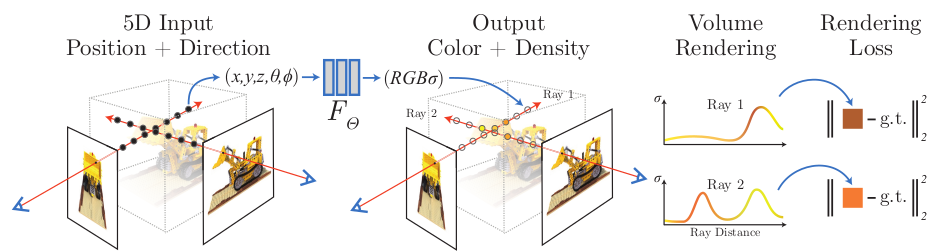
\includegraphics[width=\linewidth]{figures/c3/nerf.png}
    \caption{Kiến trúc mạng Trường bức xạ nơ-ron \cite[Fig.~2]{Mildenhall2020NeRF}.}
    \label{fig:nerf}
\end{figure}

Để đảm bảo tính nhất quán đa góc nhìn, kiến trúc mạng NeRF được minh họa ở Hình \ref{fig:nerf} được thiết kế sao cho mật độ \(\sigma\) chỉ phụ thuộc vào vị trí \(\mathbf{x}\), trong khi màu sắc \(\mathbf{c}\) phụ thuộc vào cả \(\mathbf{x}\) và \(\mathbf{d}\). Điều này phản ánh rằng mật độ (biểu thị hình học và vật liệu) không thay đổi theo hướng nhìn, nhưng màu sắc có thể thay đổi do các hiệu ứng chiếu sáng, phản xạ \cite{Mildenhall2020NeRF}.

Cụ thể, MLP \(F_{\Theta}\) xử lý tọa độ \(\mathbf{x}\) qua 8 lớp kết nối đầy đủ, mỗi lớp có 256 kênh và sử dụng hàm kích hoạt ReLU. Đầu ra của khối này gồm giá trị mật độ \(\sigma\) và một vector đặc trưng 256 chiều. Vector đặc trưng này được kết hợp với thông tin hướng nhìn \(\mathbf{d}\) và đưa qua một lớp kết nối đầy đủ (128 kênh, hàm ReLU) để dự đoán màu sắc \(\mathbf{c}\). Việc sử dụng \(\mathbf{d}\) cho phép NeRF mô phỏng các hiệu ứng thay đổi cường độ sáng, phản xạ, điều mà các mô hình chỉ dựa vào tọa độ điểm \(\mathbf{x}\) khó thực hiện.

% % --- SUBSECTION: Volume Rendering with Radiance Fields ---
% \subsection{Kết xuất thể tích với Trường bức xạ} \label{subsec:volume_rendering}

% Với biểu diễn cảnh 5D dưới dạng mật độ thể tích $\sigma(\mathbf{x})$ và bức xạ $\mathbf{c}(\mathbf{x}, \mathbf{d})$ tại mọi điểm trong không gian, NeRF sử dụng nguyên lý từ kỹ thuật kết xuất thể tích cổ điển \ref{subsec:volume_rendering_detailed}
% để tính toán màu sắc của một tia từ vị trí, hướng máy ảnh bất kỳ đi xuyên qua cảnh.

% Mật độ thể tích $\sigma(\mathbf{x})$ tại một vị trí $\mathbf{x}$ có thể được diễn giải như là xác suất vi phân mà một tia sáng kết thúc (bị hấp thụ hoặc tán xạ) tại một hạt vô cùng nhỏ ở vị trí đó. Màu sắc kỳ vọng $C(\mathbf{r})$ của một tia máy ảnh $\mathbf{r}(t) = \mathbf{o} + t\mathbf{d}$ (với $\mathbf{o}$ là gốc và $\mathbf{d}$ là hướng của tia) đi từ giới hạn gần $t_n$ đến giới hạn xa $t_f$ được tính bằng tích phân:
% \begin{equation} \label{eq:volume_rendering_integral}
% C(\mathbf{r}) = \int_{t_n}^{t_f} T(t) \sigma(\mathbf{r}(t)) \mathbf{c}(\mathbf{r}(t), \mathbf{d}) dt,
% \end{equation}
% trong đó hàm $T(t)$ biểu thị độ truyền qua tích lũy dọc theo tia từ $t_n$ đến $t$:
% \begin{equation} \label{eq:transmittance}
% T(t) = \exp\left(-\int_{t_n}^{t} \sigma(\mathbf{r}(s)) ds\right).
% \end{equation}
% $T(t)$ đại diện cho xác suất mà tia sáng có thể đi từ $t_n$ đến $t$ mà không va chạm vào bất kỳ hạt nào khác trong môi trường. Việc kết xuất một góc nhìn mới từ NeRF đòi hỏi phải ước lượng tích phân $C(\mathbf{r})$ này cho mỗi tia máy ảnh đi qua từng điểm ảnh.

% Vì hàm biểu diễn cảnh là liên tục và được định nghĩa bởi mạng nơ-ron, tích phân trong Phương trình \eqref{eq:volume_rendering_integral} không thể tính chính xác một cách giải tích. Do đó, NeRF sử dụng phương pháp cầu phương số (numerical quadrature) để xấp xỉ tích phân này. Thay vì sử dụng cầu phương xác định (deterministic quadrature) như thường làm với lưới voxel rời rạc (điều này sẽ giới hạn độ phân giải của biểu diễn liên tục), NeRF áp dụng kỹ thuật **lấy mẫu phân tầng (stratified sampling)**. Khoảng $[t_n, t_f]$ dọc theo tia được chia thành $N$ khoảng con (bins) đều nhau. Sau đó, một mẫu $t_i$ được rút ngẫu nhiên và đều từ bên trong mỗi khoảng con thứ $i$:
% \begin{equation} \label{eq:stratified_sampling}
% t_i \sim \mathcal{U}\left[t_n + \frac{i-1}{N}(t_f - t_n), t_n + \frac{i}{N}(t_f - t_n)\right].
% \end{equation}
% Mặc dù chỉ sử dụng một tập hợp hữu hạn các mẫu, việc lấy mẫu phân tầng đảm bảo rằng mạng MLP được truy vấn tại các vị trí liên tục dọc theo tia trong suốt quá trình tối ưu hóa, cho phép học được biểu diễn liên tục của cảnh [731].

% Với tập hợp các mẫu $\{t_i\}$, màu sắc của tia $\mathbf{r}$ được ước lượng bằng quy tắc cầu phương dựa trên công trình của Max \cite{Max95Optical}
% , tương tự như phép tổng hợp alpha (alpha compositing) \cite{porter1984compositing}: % Thay bằng key BibTeX
% \begin{equation} \label{eq:volume_rendering_discrete}
% \hat{C}(\mathbf{r}) = \sum_{i=1}^{N} T_i (1 - \exp(-\sigma_i \delta_i)) \mathbf{c}_i,
% \end{equation}
% trong đó $\delta_i = t_{i+1} - t_i$ là khoảng cách giữa các mẫu liền kề, $\sigma_i = \sigma(\mathbf{r}(t_i))$ và $\mathbf{c}_i = \mathbf{c}(\mathbf{r}(t_i), \mathbf{d})$ là mật độ và màu sắc được dự đoán bởi mạng $F_\Theta$ tại mẫu thứ $i$. Độ truyền qua tích lũy $T_i$ được tính rời rạc:
% \begin{equation} \label{eq:transmittance_discrete}
% T_i = \exp\left(-\sum_{j=1}^{i-1} \sigma_j \delta_j\right).
% \end{equation}
% Hệ số $(1 - \exp(-\sigma_i \delta_i))$ chính là giá trị alpha $\alpha_i$, đại diện cho độ chắn sáng (opacity) của đoạn $\delta_i$. Quan trọng là, hàm ước lượng màu $\hat{C}(\mathbf{r})$ theo công thức \eqref{eq:volume_rendering_discrete} là hoàn toàn khả vi (differentiable) đối với các đầu ra $(\sigma_i, \mathbf{c}_i)$ của mạng nơ-ron, cho phép lan truyền ngược gradient trong quá trình tối ưu hóa [732, 733].

% % --- SUBSECTION: Optimizing a Neural Radiance Field ---
% \subsection{Tối ưu hóa Trường bức xạ nơ-ron} \label{subsec:optimizing_nerf}

% Mặc dù các thành phần cốt lõi để biểu diễn cảnh và kết xuất góc nhìn mới bằng NeRF đã được mô tả, nhóm tác giả NeRF nhận thấy rằng chỉ những thành phần này là chưa đủ để đạt được chất lượng kết xuất hàng đầu cho các cảnh phức tạp [737, 738]. Do đó, họ đã giới thiệu hai cải tiến quan trọng để cho phép biểu diễn hiệu quả các cảnh có độ phân giải cao: **Mã hóa vị trí (Positional Encoding)** cho tọa độ đầu vào và **Quy trình lấy mẫu phân cấp (Hierarchical Volume Sampling)** [739].


% % --- SUBSUBSECTION: Hierarchical Volume Sampling ---
% \subsubsection{Lấy mẫu thể tích phân cấp (Hierarchical Volume Sampling)} \label{subsubsec:hierarchical_sampling}

% Chiến lược kết xuất bằng cách truy vấn mạng NeRF tại $N$ điểm lấy mẫu dày đặc dọc theo mỗi tia máy ảnh (như mô tả ở Mục \ref{subsec:volume_rendering}) là không hiệu quả về mặt tính toán. Các vùng không gian trống hoặc bị che khuất, không đóng góp vào màu sắc cuối cùng của pixel, vẫn bị lấy mẫu lặp đi lặp lại [753]. Lấy cảm hứng từ các công trình ban đầu về kết xuất thể tích \cite{Levoy90Efficient},
% NeRF đề xuất một chiến lược **lấy mẫu phân cấp (hierarchical sampling)** để tăng hiệu quả kết xuất bằng cách phân bổ các mẫu tỷ lệ thuận với đóng góp dự kiến của chúng vào kết quả cuối cùng [754].

% Thay vì chỉ sử dụng một mạng duy nhất, NeRF tối ưu hóa đồng thời hai mạng: một mạng "thô" ("coarse" network) và một mạng "tinh" ("fine" network) [755]. Quy trình hoạt động như sau:
% \begin{enumerate}
%     \item Lấy mẫu một tập hợp $N_c$ vị trí dọc theo tia bằng phương pháp lấy mẫu phân tầng (Stratified Sampling - Phương trình \eqref{eq:stratified_sampling}).
%     \item Truy vấn mạng "thô" tại $N_c$ vị trí này để có được tập các cặp $(\mathbf{c}_{c,i}, \sigma_{c,i})$.
%     \item Tính toán màu sắc ước lượng $\hat{C}_c(\mathbf{r})$ từ mạng thô bằng công thức \eqref{eq:volume_rendering_discrete}.
%     \item Dựa trên kết quả của mạng thô, tạo ra một hàm mật độ xác suất (PDF) rời rạc dọc theo tia, thiên vị về các vùng có khả năng chứa nội dung nhìn thấy được. Cụ thể, viết lại $\hat{C}_c(\mathbf{r})$ dưới dạng tổng có trọng số của các màu mẫu:
%         \begin{equation} \label{eq:hierarchical_weights}
%         \hat{C}_c(\mathbf{r}) = \sum_{i=1}^{N_c} w_i \mathbf{c}_{c,i}, \quad \text{với} \quad w_i = T_i (1 - \exp(-\sigma_{c,i} \delta_i)).
%         \end{equation}
%     Sau đó, chuẩn hóa các trọng số $w_i$ để tạo thành PDF: $\hat{w}_i = w_i / \sum_{j=1}^{N_c} w_j$ [758-760].
%     \item Rút $N_f$ mẫu vị trí thứ hai từ PDF này bằng phương pháp lấy mẫu biến đổi ngược (inverse transform sampling) [761].
%     \item Truy vấn mạng "tinh" tại tất cả $N_c + N_f$ mẫu (bao gồm cả mẫu từ bước 1 và bước 5).
%     \item Tính toán màu sắc cuối cùng $\hat{C}_f(\mathbf{r})$ bằng công thức \eqref{eq:volume_rendering_discrete} nhưng sử dụng $N_c + N_f$ mẫu và các giá trị $(\mathbf{c}_{f,i}, \sigma_{f,i})$ từ mạng tinh [761, 762].
% \end{enumerate}
% Quy trình này giúp tập trung năng lực tính toán vào các vùng không gian quan trọng, tương tự như ý tưởng của lấy mẫu theo tầm quan trọng (importance sampling), nhưng NeRF sử dụng các mẫu này để tạo ra một sự rời rạc hóa không đều của toàn bộ miền tích phân thay vì coi mỗi mẫu là một ước lượng xác suất độc lập cho toàn bộ tích phân.

% --- SUBSECTION: Volume Rendering with Radiance Fields ---
\subsection{Kết xuất thể tích với Trường bức xạ} \label{subsec:volume_rendering}

Kết xuất thể tích là một kỹ thuật cốt lõi trong phương pháp Trường bức xạ nơ-ron (NeRF), cho phép biểu diễn và tái tạo hình ảnh từ các trường bức xạ 5D liên tục. Trong NeRF, một cảnh được biểu diễn dưới dạng một hàm liên tục ánh xạ từ tọa độ không gian 3D $\mathbf{x} = (x, y, z)$ và hướng nhìn 2D $\mathbf{d} = (\theta, \phi)$ (thường được biểu diễn dưới dạng vector đơn vị 3D) đến mật độ thể tích $\sigma$ và màu sắc phát xạ phụ thuộc hướng nhìn $\mathbf{c}(\mathbf{x}, \mathbf{d}) = (r, g, b)$\cite{Mildenhall2020NeRF}. Quá trình kết xuất sử dụng các nguyên tắc của kết xuất thể tích cổ điển để tính màu sắc của một tia máy ảnh đi qua cảnh.

Màu sắc kỳ vọng $C(\mathbf{r})$ của một tia máy ảnh $\mathbf{r}(t) = \mathbf{o} + t \mathbf{d}$, với $\mathbf{o}$ là điểm xuất phát của tia, $\mathbf{d}$ là hướng tia, và $t$ nằm trong khoảng giới hạn gần và xa $[t_n, t_f]$, được tính bằng tích phân sau:

\begin{equation}
C(\mathbf{r}) = \int_{t_n}^{t_f} T(t) \sigma(\mathbf{r}(t)) \mathbf{c}(\mathbf{r}(t), \mathbf{d}) \, dt,
\end{equation}
trong đó $T(t)$ là độ truyền qua tích lũy, được định nghĩa như:

\begin{equation}\label{do_truyen_qua}
T(t) = \exp\left(-\int_{t_n}^{t} \sigma(\mathbf{r}(s)) \, ds\right).
\end{equation}

Hàm $T(t)$ biểu thị xác suất mà tia đi từ $t_n$ đến $t$ mà không va chạm với bất kỳ hạt nào, tức là xác suất tia không bị chặn. Mật độ thể tích $\sigma(\mathbf{r}(t))$ được xem như xác suất vi phân của việc tia bị chấm dứt tại vị trí $\mathbf{r}(t)$, và $\mathbf{c}(\mathbf{r}(t))$.

Để ước lượng số tích phân liên tục này, NeRF sử dụng phương pháp lấy mẫu phân tầng. Khoảng $[t_n, t_f]$ được chia thành $N$ đoạn đều nhau, và một mẫu được rút ngẫu nhiên từ mỗi đoạn:

\begin{equation}
t_i \sim \mathcal{U}\left[t_n + \frac{i-1}{N}(t_f - t_n), t_n + \frac{i}{N}(t_f - t_n)\right].
\end{equation}

Phương pháp này cho phép biểu diễn cảnh liên tục, vì mạng nơ-ron được truy vấn tại các vị trí liên tục trong suốt quá trình tối ưu hóa. Màu sắc được ước lượng bằng quy tắc xấp xỉ tích phân:

\begin{equation}\label{color_cumulative}
\hat{C}(\mathbf{r}) = \sum_{i=1}^N T_i \left(1 - \exp(-\sigma_i \delta_i)\right) \mathbf{c}_i,
\end{equation}
trong đó $T_i = \exp\left(-\sum_{j=1}^{i-1} \sigma_j \delta_j\right)$, và $\delta_i = t_{i+1} - t_i$ là khoảng cách giữa các mẫu liền kề. Công thức \ref{color_cumulative} tương đương với phép tổng hợp alpha truyền thống với $\alpha_i = 1 - \exp(-\sigma_i \delta_i)$, đảm bảo hàm kết xuất là khả vi, cho phép tối ưu hóa dựa trên gradient.

\subsection{Tối ưu hóa Trường bức xạ nơ-ron} \label{subsec:optimizing_nerf}

Việc tối ưu hóa NeRF bao gồm việc điều chỉnh các tham số $\Theta$ của mạng MLP $F_\Theta: (\mathbf{x}, \mathbf{d}) \to (\mathbf{c}, \sigma)$ để giảm thiểu sai số giữa các hình ảnh quan sát và các hình ảnh được kết xuất từ biểu diễn trường bức xạ. Quá trình này sử dụng giảm gradient với hàm mất mát là tổng bình phương sai số giữa màu sắc dự đoán và màu sắc thực tế:

\begin{equation}
\mathcal{L} = \sum_{\mathbf{r} \in \mathcal{R}} \left[ \left\| \hat{C}_c(\mathbf{r}) - C(\mathbf{r}) \right\|_2^2 + \left\| \hat{C}_f(\mathbf{r}) - C(\mathbf{r}) \right\|_2^2 \right],
\end{equation}
trong đó $\mathcal{R}$ là tập hợp các tia trong mỗi lô, $\hat{C}_c(\mathbf{r})$ và $\hat{C}_f(\mathbf{r})$ lần lượt là màu sắc dự đoán từ mạng thô và mạng tinh, và $C(\mathbf{r})$ là màu sắc thực tế. Hàm mất mát này khuyến khích mạng dự đoán mật độ thể tích cao và màu sắc chính xác tại các vị trí chứa nội dung cảnh thực.

Để cải thiện hiệu suất, NeRF sử dụng mã hóa vị trí để ánh xạ tọa độ đầu vào vào không gian chiều cao hơn giúp mạng học đặc trưng về vị trí trong không gian tốt hơn. Hàm mã hóa vị trí $\gamma(p)$ được định nghĩa như:

\begin{equation}
\gamma(p) = \left( \sin(2^0 \pi p), \cos(2^0 \pi p), \ldots, \sin(2^{L-1} \pi p), \cos(2^{L-1} \pi p) \right),
\end{equation}
với $L=10$ cho tọa độ không gian $\mathbf{x}$ và $L=4$ cho hướng nhìn $\mathbf{d}$. Hàm này được áp dụng riêng cho mỗi thành phần của $\mathbf{x}$ và $\mathbf{d}$, sau khi được chuẩn hóa về $[-1, 1]$. Mã hóa vị trí cải thiện đáng kể khả năng biểu diễn chi tiết hình học và màu sắc của mô hình.

Ngoài ra, NeRF sử dụng một quy trình lấy mẫu phân cấp (xem Mục \ref{subsubsec:hierarchical_sampling}) để phân bổ hiệu quả các mẫu vào các vùng có nội dung cảnh quan trọng.

\subsection{Lấy mẫu phân cấp} \label{subsubsec:hierarchical_sampling}

Lấy mẫu phân cấp là một cải tiến quan trọng trong NeRF để tăng hiệu quả kết xuất bằng cách phân bổ các mẫu một cách thông minh vào các vùng có khả năng chứa nội dung cảnh hữu ích. Thay vì chỉ sử dụng một mạng duy nhất, NeRF tối ưu hóa đồng thời hai mạng: một mạng "thô" và một mạng "tinh".

Đầu tiên, $N_c$ điểm được lấy mẫu bằng phương pháp phân tầng và được đánh giá bởi mạng thô. Kết quả từ mạng thô được sử dụng để tạo ra một phân phối xác suất dọc theo tia, dựa trên trọng số của các mẫu:

\begin{equation}
\hat{C}_c(\mathbf{r}) = \sum_{i=1}^{N_c} w_i \mathbf{c}_i, \quad w_i = T_i \left(1 - \exp(-\sigma_i \delta_i)\right),
\end{equation}
trong đó $w_i$ là trọng số của mẫu thứ $i$, và $T_i$ được tính như trong công thức \ref{do_truyen_qua}. Các trọng số này được chuẩn hóa $\hat{w}_i = w_i / \sum_{j=1}^{N_c} w_j$ thành một hàm mật độ xác suất phân đoạn hằng số.

Tiếp theo, $N_f$ điểm bổ sung được lấy mẫu từ phân phối này bằng phương pháp lấy mẫu nghịch đảo. Mạng tinh sau đó được đánh giá tại tập hợp hợp nhất của $N_c + N_f$ điểm, và màu sắc cuối cùng $\hat{C}_f(\mathbf{r})$ được tính bằng công thức \ref{color_cumulative} sử dụng tất cả các mẫu này. Quy trình này đảm bảo rằng nhiều mẫu hơn được phân bổ cho các vùng được suy đoán là có nội dung cảnh quan trọng, cải thiện hiệu quả và chất lượng kết xuất mà không làm tăng đáng kể chi phí tính toán.

Trong triển khai, NeRF sử dụng $N_c = 64$ mẫu cho mạng thô và $N_f = 128$ mẫu bổ sung cho mạng tinh, với kích thước lô là 4096 tia. Tối ưu hóa được thực hiện bằng bộ tối ưu Adam với tốc độ học ban đầu là $5 \times 10^{-4}$, giảm dần theo hàm mũ đến $5 \times 10^{-5}$ trong suốt 100-300 nghìn lần lặp.

% --- SUBSUBSECTION: Positional Encoding ---
\subsubsection{Mã hóa vị trí} \label{subsubsec:positional_encoding}

Thực nghiệm cho thấy rằng việc cho mạng nơ-ron $F_{\Theta}$ hoạt động trực tiếp trên các tọa độ 5D $(\mathbf{x}, \mathbf{d})$ ban đầu dẫn đến kết quả kết xuất kém trong việc biểu diễn các chi tiết có tần số biến đổi cao về màu sắc và hình học. Điều này phù hợp với các nghiên cứu trước đó chỉ ra rằng các mạng nơ-ron sâu có xu hướng thiên vị học các hàm tần số thấp trước - tức là các hàm có thay đổi giá trị rất nhanh trong một khoảng ngắn \cite{Rahaman18Spectral}. Các nghiên cứu này cũng cho thấy việc ánh xạ đầu vào lên một không gian có số chiều cao hơn bằng cách sử dụng các hàm tần số cao trước khi đưa vào mạng có thể giúp mạng học tốt hơn các dữ liệu chứa biến đổi tần số cao.

NeRF tận dụng phát hiện này bằng cách biến đổi tọa độ đầu vào 5D thông qua một hàm mã hóa vị trí $\gamma(\cdot)$ trước khi đưa vào mạng MLP. Cụ thể, mạng $F_\Theta$ được xem như là hợp của hai hàm $F_\Theta = F'_\Theta \circ \gamma$, trong đó $\gamma$ là hàm mã hóa cố định (không học) và $F'_\Theta$ vẫn là mạng MLP thông thường. Hàm mã hóa được sử dụng có dạng:
\begin{equation} \label{eq:positional_encoding}
\gamma(p) = \left( \sin(2^0 \pi p), \cos(2^0 \pi p), \dots, \sin(2^{L-1} \pi p), \cos(2^{L-1} \pi p) \right).
\end{equation}
Hàm $\gamma(\cdot)$ này ánh xạ một giá trị vô hướng $p$ vào một không gian $\mathbb{R}^{2L}$. Nó được áp dụng riêng biệt cho từng thành phần của tọa độ vị trí $\mathbf{x} = (x, y, z)$ (thường được chuẩn hóa về khoảng [-1, 1]) và từng thành phần của vector hướng nhìn đơn vị $\mathbf{d}$. Kỹ thuật ánh xạ này giúp mạng MLP dễ dàng xấp xỉ các hàm tần số biến đổi cao hơn, cải thiện đáng kể khả năng biểu diễn chi tiết của cảnh.

% \section{Một vài biến thể cải tiến của NeRF}

% Kể từ khi Trường bức xạ nơ-ron (NeRF) được giới thiệu, nhiều biến thể cải tiến đã được đề xuất để giải quyết các hạn chế về hiệu quả tính toán, chất lượng tái tạo, và khả năng biểu diễn các đặc tính hình học phức tạp. Phần này khảo sát ba biến thể nổi bật: Mip-NeRF, Instant-NGP, và NeuS, tập trung vào các kỹ thuật cải tiến, công thức toán học cốt lõi, và những cải tiến so với NeRF gốc.

% \subsection{Mip-NeRF}

% \textbf{Kỹ thuật cải tiến:} Mip-NeRF \cite{barron2021mip} giải quyết vấn đề suy giảm chất lượng hình ảnh khi kết xuất ở các độ phân giải khác nhau hoặc với các tia có kích thước lớn (ví dụ, khi sử dụng hình ảnh ở độ phân giải thấp hoặc siêu phân giải). NeRF gốc giả định các tia là vô cực mỏng, dẫn đến hiện tượng "răng cưa" khi tích hợp trên các vùng điểm ảnh. Mip-NeRF thay thế truy vấn điểm đơn bằng tích hợp trên hình nón tia, sử dụng biểu diễn tích phân trường bức xạ để mã hóa các vùng không gian thay vì các điểm riêng lẻ.

% \textbf{Công thức toán học:} Thay vì truy vấn trường bức xạ tại một điểm $\mathbf{x}$, mip-NeRF sử dụng một phân phối Gaussian trên hình nón tia, với kỳ vọng màu sắc được tính như:

% \begin{equation}
% C(\mathbf{r}) = \int T(t) \sigma(\mathbf{r}(t)) \mathbf{c}(\mathbf{r}(t), \mathbf{d}) \mathcal{N}(\mathbf{r}(t); \mu(t), \Sigma(t)) \, dt,
% \end{equation}
% trong đó $\mathcal{N}(\mathbf{r}(t); \mu(t), \Sigma(t))$ là phân phối Gaussian mô tả độ không chắc chắn của vị trí trên hình nón tia tại $t$, và IPE ánh xạ các tham số $\mu(t), \Sigma(t)$ vào không gian chiều cao hơn.

% \textbf{Cải thiện:} mip-NeRF giảm hiện tượng aliasing, cải thiện chất lượng kết xuất trên các độ phân giải đa dạng, và giảm sai số tái tạo (PSNR cao hơn khoảng 17\% so với NeRF trên các tập dữ liệu đa tỷ lệ). Nó cũng giảm số lượng mẫu cần thiết, tăng hiệu quả tính toán.

% \subsection{Instant-NGP}

% \textbf{Kỹ thuật cải tiến:} Instant Neural Graphics Primitives (Instant-NGP) \cite{muller2022instant} tập trung vào việc tăng tốc độ huấn luyện và kết xuất của NeRF bằng cách sử dụng một cấu trúc dữ liệu đa độ phân giải (multiresolution hash encoding) thay vì mạng MLP lớn. Biểu diễn trường bức xạ được lưu trữ trong một bảng băm (hash table) với các đặc trưng được nội suy tại các độ phân giải khác nhau, kết hợp với một MLP nhỏ để dự đoán mật độ và màu sắc.

% \textbf{Công thức toán học:} Hàm trường bức xạ được biểu diễn như:

% \begin{equation}
% (\mathbf{c}, \sigma) = F_\Theta(\gamma(\mathbf{x}), \mathbf{d}),
% \end{equation}
% trong đó $\gamma(\mathbf{x})$ là hàm mã hóa băm đa độ phân giải, ánh xạ tọa độ $\mathbf{x}$ thành một tập hợp đặc trưng nội suy từ các mức độ phân giải trong bảng băm, và $F_\Theta$ là một MLP nhỏ.

% \textbf{Cải thiện:} Instant-NGP giảm đáng kể thời gian huấn luyện (từ vài ngày xuống vài phút) và tăng tốc độ kết xuất (đạt tốc độ thời gian thực trên GPU). Nó duy trì hoặc vượt trội chất lượng hình ảnh của NeRF gốc, với chi phí lưu trữ thấp hơn và khả năng xử lý các cảnh lớn hơn.

% \subsection{NeuS}

% \textbf{Kỹ thuật cải tiến:} Neural Implicit Surfaces (NeuS) \cite{wang2021neus} cải thiện khả năng tái tạo bề mặt hình học chính xác bằng cách biểu diễn cảnh dưới dạng hàm khoảng cách có dấu (Signed Distance Function - SDF) thay vì trường mật độ thể tích như NeRF. NeuS sử dụng một hàm trọng số dựa trên phân phối logistic để chuyển đổi SDF thành mật độ thể tích, đảm bảo tái tạo bề mặt mịn và chính xác hơn.

% \textbf{Công thức toán học:} Hàm SDF $f(\mathbf{x})$ được ánh xạ thành mật độ thể tích thông qua:

% \begin{equation}
% \sigma(\mathbf{x}) = \frac{1}{\beta} \cdot \frac{\exp(-f(\mathbf{x})/\beta)}{(1 + \exp(-f(\mathbf{x})/\beta))^2},
% \end{equation}
% trong đó $\beta$ là tham số kiểm soát độ mịn của chuyển đổi. Màu sắc và mật độ sau đó được tích hợp dọc theo tia tương tự NeRF:

% \begin{equation}
% C(\mathbf{r}) = \int T(t) \sigma(\mathbf{r}(t)) \mathbf{c}(\mathbf{r}(t), \mathbf{d}) \, dt.
% \end{equation}

% \textbf{Cải thiện:} NeuS cung cấp tái tạo bề mặt chất lượng cao hơn NeRF, đặc biệt với các hình học phức tạp, nhờ biểu diễn SDF đảm bảo tính liên tục và tính chất bề mặt rõ ràng. Nó giảm hiện tượng "mây mù" (fog artifacts) trong không gian trống và cải thiện độ chính xác hình học (đo bằng sai số Chamfer Distance).


% \section{NeuS}
Tái tạo bề mặt 3D từ ảnh đa góc nhìn là một bài toán cốt lõi trong thị giác máy tính và đồ họa máy tính \cite{Wang2021NeuS}. Các phương pháp biểu diễn ngầm neural (neural implicit representations) gần đây cho thấy nhiều hứa hẹn nhờ khả năng tạo ra kết quả chất lượng cao và xử lý các trường hợp phức tạp như bề mặt không Lambertian hay cấu trúc mỏng \cite{Wang2021NeuS}. Tuy nhiên, các phương pháp hiện tại còn tồn tại những hạn chế nhất định.

\subsection{Hạn chế của các phương pháp trước NeuS}

Có hai hướng tiếp cận chính trước NeuS:

\begin{itemize}
    \item \textbf{Phương pháp dựa trên Surface Rendering (ví dụ: IDR \cite{Yariv2020IDR}, DVR \cite{Niemeyer2020DVR}):} Các phương pháp này thường biểu diễn bề mặt dưới dạng hàm chiếm dụng (occupancy) hoặc hàm khoảng cách có dấu (Signed Distance Function - SDF). Chúng sử dụng kỹ thuật surface rendering khả vi để huấn luyện mạng neural bằng cách so sánh ảnh render với ảnh đầu vào. Mặc dù IDR cho kết quả ấn tượng, nó gặp khó khăn với các cấu trúc phức tạp gây thay đổi độ sâu đột ngột. Nguyên nhân là do surface rendering chỉ xem xét một điểm giao duy nhất của tia nhìn với bề mặt, khiến gradient chỉ tồn tại cục bộ, dễ bị mắc kẹt ở cực tiểu địa phương. Thêm vào đó, các phương pháp này thường yêu cầu mặt nạ vật thể (foreground mask) để giám sát và hội tụ \cite{Wang2021NeuS}. % Source [2], [12-14], [16], [51]
    \item \textbf{Phương pháp dựa trên Volume Rendering (ví dụ: NeRF \cite{Mildenhall2020NeRF}):} Các phương pháp này biểu diễn cảnh dưới dạng trường bức xạ (radiance field) và mật độ thể tích (volume density). Chúng sử dụng volume rendering bằng cách lấy mẫu nhiều điểm dọc theo tia nhìn và tổng hợp màu sắc ($\alpha$-composition) để tạo ra màu pixel. Ưu điểm là khả năng xử lý thay đổi độ sâu đột ngột tốt hơn do gradient được lan truyền từ nhiều điểm. Tuy nhiên, NeRF được thiết kế chính cho tổng hợp ảnh nhìn mới (novel view synthesis), việc trích xuất bề mặt chất lượng cao từ trường mật độ học được là rất khó khăn do thiếu các ràng buộc hình học rõ ràng trên bề mặt. Bề mặt trích xuất từ NeRF thường bị nhiễu \cite{Wang2021NeuS}. % Source [3], [19-23], [52], [54]
\end{itemize}

\subsection{Phương pháp NeuS}

NeuS (Neural Surfaces) được đề xuất để khắc phục những hạn chế trên bằng cách kết hợp các ưu điểm của cả hai hướng tiếp cận: biểu diễn bề mặt chính xác bằng SDF và tối ưu mạnh mẽ bằng volume rendering \cite{Wang2021NeuS}. % Source [1], [29], [31], [55]

\subsubsection{Biểu diễn cảnh}
NeuS biểu diễn hình học của vật thể bằng một hàm SDF $f: \mathbb{R}^3 \to \mathbb{R}$ và biểu diễn màu sắc (appearance) bằng một hàm $c: \mathbb{R}^3 \times \mathbb{S}^2 \to \mathbb{R}^3$, cả hai đều được mã hóa bởi mạng MLP. Bề mặt $\mathcal{S}$ được định nghĩa là tập mức 0 của SDF: $\mathcal{S} = \{x \in \mathbb{R}^3 | f(x) = 0\}$ \cite{Wang2021NeuS}. % Source [5], [30], [60], [63], [64]

\subsubsection{Volume Rendering cho SDF}
Để áp dụng volume rendering cho việc huấn luyện mạng SDF, NeuS giới thiệu một hàm mật độ xác suất $\phi_s(f(x))$, gọi là \textbf{S-density}, được định nghĩa dựa trên giá trị SDF tại điểm $x$. Hàm $\phi_s$ thường được chọn là hàm mật độ logistic (đạo hàm của hàm sigmoid $\Phi_s(x)=(1+e^{-sx})^{-1}$), có dạng hình chuông tập trung tại $f(x)=0$. Tham số $1/s$ thể hiện độ lệch chuẩn và cũng là một tham số có thể học được \cite{Wang2021NeuS}. % Source [65-70]

Màu sắc của một pixel $C(o,v)$ được tính bằng tích phân màu $c(p(t), v)$ dọc theo tia nhìn $p(t) = o + tv$ với một hàm trọng số $w(t)$:
$$C(o,v) = \int_{0}^{+\infty} w(t) c(p(t), v) dt$$
\cite{Wang2021NeuS}. % Source [72], [73]

\subsubsection{Hàm Trọng số Volume Rendering Không Lệch (Unbiased)}
Việc xây dựng hàm trọng số $w(t)$ phù hợp là chìa khóa. NeuS chỉ ra rằng việc áp dụng công thức volume rendering tiêu chuẩn một cách "ngây thơ" sẽ dẫn đến sai lệch (bias) hình học. Để giải quyết vấn đề này, NeuS đề xuất một công thức volume rendering mới, đảm bảo tính \textbf{không lệch (unbiased)} (trọng số cực đại tại bề mặt SDF=0) và \textbf{nhận biết che khuất (occlusion-aware)} \cite{Wang2021NeuS}. % Source [6], [32], [74-80], [83-87]

NeuS định nghĩa một hàm "mật độ mờ đục" (opaque density) $\rho(t)$ mới từ S-density $\phi_s$ và CDF $\Phi_s$ của nó:
$$\rho(t) = \max\left(\frac{-\frac{d\Phi_s}{dt}(f(p(t)))}{\Phi_s(f(p(t)))}, 0\right)$$
và tính trọng số $w(t) = T(t)\rho(t)$. Hàm trọng số này được chứng minh là không lệch trong xấp xỉ bậc nhất \cite{Wang2021NeuS}. % Source [90-94], [101-103], [105-109], [111-114]

Trong quá trình rời rạc hóa, giá trị alpha $\alpha_i$ cho đoạn $[t_i, t_{i+1}]$ được tính bằng:
$$\alpha_i = \max\left(\frac{\Phi_s(f(p(t_i))) - \Phi_s(f(p(t_{i+1})))}{\Phi_s(f(p(t_i)))}, 0\right)$$
\cite{Wang2021NeuS}. % Source [115], [116], [263-266]

\subsubsection{Huấn luyện}
NeuS được huấn luyện bằng cách tối thiểu hóa hàm mất mát bao gồm $\mathcal{L}_{color}$ (L1 loss giữa màu render và ảnh gốc), $\mathcal{L}_{reg}$ (ràng buộc Eikonal: $\|\nabla f(x)\|_2 = 1$) và tùy chọn $\mathcal{L}_{mask}$ (nếu có mask) \cite{Wang2021NeuS}. % Source [117-119], [121-124]
NeuS cũng sử dụng chiến lược lấy mẫu phân cấp (hierarchical sampling) \cite{Wang2021NeuS}. % Source [124], [125]

\subsection{Kết quả và Ưu điểm}
Các thí nghiệm trên bộ dữ liệu DTU \cite{Jensen2014DTU} và BlendedMVS \cite{Yao2020BlendedMVS} cho thấy NeuS vượt trội hơn các phương pháp tiên tiến như IDR \cite{Yariv2020IDR}, NeRF \cite{Mildenhall2020NeRF}, COLMAP \cite{Schonberger16SFMRevisited} (hoặc \cite{Schoenberger2016Pixelwise}) và UNISURF \cite{Oechsle2021UNISURF} về chất lượng tái tạo bề mặt, đặc biệt đối với các đối tượng có cấu trúc phức tạp, tự che khuất và cấu trúc mỏng. Đáng chú ý, NeuS đạt được kết quả tốt ngay cả khi không cần sử dụng mask giám sát \cite{Wang2021NeuS}. % Source [7], [28], [35], [147], [149], [173], [178]

Tóm lại, NeuS là một phương pháp hiệu quả để tái tạo bề mặt 3D chất lượng cao từ ảnh đa góc nhìn, giải quyết được các hạn chế của các phương pháp trước đó bằng cách kết hợp biểu diễn SDF và một cơ chế volume rendering mới, không lệch.


\section{Instant-NGP}
Các phương pháp biểu diễn đồ họa dựa trên mạng neural (neural graphics primitives), thường sử dụng Multi-Layer Perceptrons (MLP) để tham số hóa các hàm biểu diễn hình dạng (ví dụ: SDF \cite{Park2019DeepSDF}) hoặc trường bức xạ (ví dụ: NeRF \cite{Mildenhall2020NeRF}), đã đạt được những thành tựu ấn tượng \cite{Muller2022InstantNGP}. Tuy nhiên, việc huấn luyện và tính toán các MLP lớn thường tốn kém tài nguyên và thời gian \cite{Muller2022InstantNGP_source_8}. Các kỹ thuật mã hóa đầu vào (input encoding) như mã hóa tần số (frequency encoding) \cite{Mildenhall2020NeRF, Vaswani2017Attention} giúp cải thiện chất lượng nhưng vẫn đòi hỏi MLP lớn và hội tụ chậm \cite{Muller2022InstantNGP_source_78}. Các phương pháp mã hóa tham số (parametric encoding) sử dụng cấu trúc dữ liệu phụ trợ như lưới dày (dense grid) hoặc cây (tree) \cite{Liu2020NSVF, Takikawa2021NGLOD} có thể tăng tốc huấn luyện bằng cách giảm kích thước MLP, nhưng lại gặp vấn đề về bộ nhớ lớn hoặc yêu cầu các thuật toán cập nhật cấu trúc phức tạp (pruning, merging), không hiệu quả trên GPU hiện đại \cite{Muller2022InstantNGP_source_26, Muller2022InstantNGP_source_28, Muller2022InstantNGP_source_55, Muller2022InstantNGP_source_74, Muller2022InstantNGP_source_81, Muller2022InstantNGP_source_92}.

Để giải quyết những thách thức này, Müller và cộng sự đã đề xuất Instant Neural Graphics Primitives (Instant-NGP), một phương pháp đột phá dựa trên kỹ thuật mã hóa đầu vào mới gọi là \textbf{Multiresolution Hash Encoding} (Mã hóa Băm Đa Phân giải) \cite{Muller2022InstantNGP}. Ý tưởng cốt lõi là thay thế MLP lớn bằng một MLP \textit{nhỏ} kết hợp với một cấu trúc dữ liệu hiệu quả chứa các tham số có thể huấn luyện được \cite{Muller2022InstantNGP_source_9}.

\subsection{Phương pháp Multiresolution Hash Encoding}

Mã hóa băm đa phân giải hoạt động như sau (xem Hình 3 trong \cite{Muller2022InstantNGP}):
\begin{enumerate}
    \item \textbf{Cấu trúc đa mức (Multiresolution Levels):} Sử dụng $L$ (thường là 16) mức phân giải khác nhau. Mỗi mức $l$ tương ứng với một lưới ảo (virtual grid) có độ phân giải $N_l$, tăng dần theo cấp số nhân từ $N_{min}$ đến $N_{max}$ \cite{Muller2022InstantNGP_source_112, Muller2022InstantNGP_source_113, Muller2022InstantNGP_source_114}.
    \item \textbf{Bảng băm đặc trưng (Feature Hash Tables):} Mỗi mức $l$ được liên kết với một bảng (mảng) chứa tối đa $T$ vector đặc trưng (feature vectors) $F$-chiều (thường $F=2$), gọi là $\theta_l$. $T$ là một siêu tham số quan trọng, cân bằng giữa chất lượng, bộ nhớ và hiệu năng \cite{Muller2022InstantNGP_source_105, Muller2022InstantNGP_source_112, Muller2022InstantNGP_source_125}.
    \item \textbf{Tra cứu và Băm (Lookup and Hashing):} Với một tọa độ đầu vào $x \in \mathbb{R}^d$, tại mỗi mức $l$:
        \begin{itemize}
            \item Xác định các đỉnh (corners) $2^d$ của ô lưới ảo (voxel) bao quanh $x$.
            \item Ánh xạ tọa độ nguyên của các đỉnh này tới các chỉ số (indices) trong bảng đặc trưng $\theta_l$:
                \begin{itemize}
                    \item Ở các mức phân giải thô (số đỉnh lưới $\le T$): Ánh xạ 1-1.
                    \item Ở các mức phân giải mịn (số đỉnh lưới $> T$): Sử dụng một hàm băm không gian (spatial hash function), ví dụ $h(\mathbf{x}) = (\bigoplus_{i=1}^d x_i \pi_i) \pmod T$, để lấy chỉ số \cite{Muller2022InstantNGP_source_104, Muller2022InstantNGP_source_117, Muller2022InstantNGP_source_118, Muller2022InstantNGP_source_121, Teschner2003SpatialHashing}.
                \end{itemize}
        \end{itemize}
    \item \textbf{Xử lý Xung đột Băm (Collision Handling):} Instant-NGP \textit{không} sử dụng các cơ chế xử lý xung đột băm tường minh. Thay vào đó, nó dựa vào hai yếu tố:
        \begin{itemize}
            \item Tối ưu hóa dựa trên gradient: Khi nhiều vị trí bị băm vào cùng một mục trong bảng, gradient của chúng sẽ được cộng dồn (hoặc trung bình). Gradient từ các mẫu "quan trọng" hơn (ví dụ: điểm trên bề mặt nhìn thấy trong NeRF) sẽ chiếm ưu thế và điều khiển giá trị của mục đó \cite{Muller2022InstantNGP_source_34, Muller2022InstantNGP_source_150, Muller2022InstantNGP_source_153}.
            \item Mạng MLP theo sau: Mạng neural nhỏ $m$ học cách phân giải các xung đột còn lại bằng cách kết hợp thông tin từ nhiều mức phân giải (các mức thô thường không có xung đột) \cite{Muller2022InstantNGP_source_99, Muller2022InstantNGP_source_119, Muller2022InstantNGP_source_142, Muller2022InstantNGP_source_149}.
        \end{itemize}
    \item \textbf{Nội suy và Kết hợp (Interpolation and Concatenation):} Các vector đặc trưng $F$-chiều được lấy ra từ bảng băm tại các đỉnh voxel được nội suy tuyến tính đa chiều (d-linear interpolation) dựa trên vị trí tương đối của $x$ trong voxel đó \cite{Muller2022InstantNGP_source_105, Muller2022InstantNGP_source_123}. Kết quả nội suy từ tất cả $L$ mức được nối (concatenate) lại với nhau (cùng các đầu vào phụ trợ $\xi$ như hướng nhìn nếu cần) để tạo thành vector đầu vào $y$ cho MLP $m(y; \Phi)$ \cite{Muller2022InstantNGP_source_106, Muller2022InstantNGP_source_124}.
\end{enumerate}

\subsection{Ưu điểm và Cài đặt}

Cách tiếp cận này mang lại nhiều lợi ích đáng kể:
\begin{itemize}
    \item \textbf{Tốc độ huấn luyện cực nhanh:} Cho phép huấn luyện các biểu diễn neural chất lượng cao chỉ trong vài giây đến vài phút trên một GPU duy nhất, nhanh hơn nhiều bậc độ lớn so với các phương pháp trước đó \cite{Muller2022InstantNGP_source_1, Muller2022InstantNGP_source_6, Muller2022InstantNGP_source_16, Muller2022InstantNGP_source_131, Muller2022InstantNGP_source_293, Muller2022InstantNGP_source_345}.
    \item \textbf{Hiệu năng tính toán cao:} Render thời gian thực (vài chục ms ở độ phân giải HD) \cite{Muller2022InstantNGP_source_16, Muller2022InstantNGP_source_255, Muller2022InstantNGP_source_272}.
    \item \textbf{Chất lượng cao:} Đạt được chất lượng tương đương hoặc tốt hơn các phương pháp SOTA như NeRF, mip-NeRF, NSVF, NGLOD trong nhiều tác vụ \cite{Muller2022InstantNGP_source_6, Muller2022InstantNGP_source_30, Muller2022InstantNGP_source_138, Muller2022InstantNGP_source_216, Muller2022InstantNGP_source_292}.
    \item \textbf{Tính linh hoạt và Đơn giản:} Mã hóa không phụ thuộc tác vụ, dễ cấu hình (chủ yếu qua $T$), không cần cơ chế cập nhật cấu trúc dữ liệu phức tạp \cite{Muller2022InstantNGP_source_7, Muller2022InstantNGP_source_29, Muller2022InstantNGP_source_36, Muller2022InstantNGP_source_94, Muller2022InstantNGP_source_195, Muller2022InstantNGP_source_343}. Tự động thích ứng với phân bố dữ liệu \cite{Muller2022InstantNGP_source_158, Muller2022InstantNGP_source_159}.
    \item \textbf{Hiệu quả trên GPU:} Cấu trúc bảng băm dễ song song hóa, tra cứu $O(1)$, tận dụng cache hiệu quả. Toàn bộ hệ thống được cài đặt bằng các CUDA kernel hợp nhất (fully-fused) trong framework \texttt{tiny-cuda-nn} \cite{Muller2021TinyCuDNN, Muller2022InstantNGP_source_15, Muller2022InstantNGP_source_37, Muller2022InstantNGP_source_38, Muller2022InstantNGP_source_39, Muller2022InstantNGP_source_100, Muller2022InstantNGP_source_167}.
\end{itemize}

Instant-NGP sử dụng MLP rất nhỏ (thường chỉ 2 lớp ẩn, 64 neuron) \cite{Muller2022InstantNGP_source_178}, lưu trữ đặc trưng dạng half-precision, tối ưu bằng Adam với $\epsilon$ nhỏ ($10^{-15}$) \cite{Kingma2014Adam, Muller2022InstantNGP_source_168, Muller2022InstantNGP_source_184}. Đối với NeRF, nhóm tác giả sử dụng kiến trúc gồm MLP mật độ và MLP màu, kết hợp occupancy grid để tăng tốc ray marching \cite{Muller2022InstantNGP_source_262, Muller2022InstantNGP_source_270, Muller2022InstantNGP_source_490}.

\subsection{Ứng dụng và Hạn chế}

Instant-NGP đã được chứng minh hiệu quả trên nhiều tác vụ như biểu diễn ảnh gigapixel, học hàm SDF, Neural Radiance Caching \cite{Muller2021NRC}, và đặc biệt là NeRF \cite{Muller2022InstantNGP_source_1}. Nó cho phép huấn luyện NeRF chất lượng cao nhanh hơn 20-60 lần so với frequency encoding trên cùng implementation tối ưu \cite{Muller2022InstantNGP_source_281, Muller2022InstantNGP_source_299}.

Một hạn chế nhỏ là hiện tượng nhiễu hạt (microstructure/graininess) có thể xuất hiện do xung đột băm, đặc biệt rõ trên bề mặt SDF \cite{Muller2022InstantNGP_source_228, Muller2022InstantNGP_source_245, Muller2022InstantNGP_source_328}.

Nhìn chung, Instant-NGP với mã hóa băm đa phân giải là một bước tiến quan trọng, cung cấp một giải pháp thay thế hiệu quả, nhanh chóng và linh hoạt cho các cấu trúc dữ liệu và MLP lớn trong lĩnh vực neural graphics primitives.
\section{NeuS2}
Chắc chắn rồi, dựa trên bài báo bạn cung cấp về NeuS2, tôi đã tổng hợp thông tin tập trung vào phương pháp, ưu nhược điểm và chuẩn bị một section LaTeX cùng file BibTeX tương ứng.

1. Mã LaTeX cho Section trong Luận văn:

Đoạn mã

\section{NeuS2: Học Nhanh Bề Mặt Ngầm Neural để Tái tạo Đa Góc nhìn}

Các phương pháp tái tạo bề mặt 3D dựa trên biểu diễn ngầm neural, như NeuS \cite{Wang2021NeuS}, đã chứng minh khả năng tạo ra kết quả chất lượng rất cao cho cảnh tĩnh \cite{Wang2023NeuS2_source_1}. Tuy nhiên, một hạn chế lớn của NeuS là thời gian huấn luyện cực kỳ dài (khoảng 8 giờ), khiến nó gần như không thể áp dụng cho các cảnh động với hàng nghìn khung hình \cite{Wang2023NeuS2_source_2, Wang2023NeuS2_source_17}. Mặt khác, các phương pháp tăng tốc như Instant-NGP \cite{Muller2022InstantNGP} tuy nhanh nhưng chất lượng hình học trích xuất từ trường mật độ (density field) lại bị nhiễu và thiếu các ràng buộc bề mặt \cite{Wang2023NeuS2_source_19, Wang2023NeuS2_source_94}. Việc kết hợp trực tiếp NeuS và Instant-NGP gặp thách thức lớn trong việc tính toán hiệu quả đạo hàm bậc hai (cần thiết cho ràng buộc Eikonal của NeuS) khi sử dụng các MLP được tối ưu hóa cao bằng CUDA \cite{Wang2023NeuS2_source_23, Wang2023NeuS2_source_24, Wang2023NeuS2_source_95, Wang2023NeuS2_source_96, Wang2023NeuS2_source_97, Wang2023NeuS2_source_98}.

NeuS2 \cite{Wang2023NeuS2} được đề xuất để giải quyết những vấn đề này, nhằm mục tiêu học nhanh các bề mặt ngầm neural chất lượng cao từ ảnh đa góc nhìn cho cả cảnh tĩnh và động.

\subsection{Phương pháp Mô hình NeuS2}

NeuS2 kế thừa ý tưởng biểu diễn bề mặt bằng hàm khoảng cách có dấu (SDF) và cơ chế volume rendering không lệch (unbiased) từ NeuS \cite{Wang2021NeuS}, đồng thời tích hợp các kỹ thuật tăng tốc từ Instant-NGP \cite{Muller2022InstantNGP} và đề xuất các cải tiến mới.

\subsubsection{Kiến trúc cho Cảnh tĩnh}
\begin{itemize}
    \item \textbf{Biểu diễn kết hợp SDF và Hash Encoding:} Thay vì dùng MLP lớn, NeuS2 sử dụng một MLP \textit{nhỏ} để học hàm SDF $f$. Đầu vào của MLP này là sự kết hợp (concatenate) của tọa độ điểm 3D $x$ và vector đặc trưng $h_\Omega(x)$ được truy vấn từ cấu trúc mã hóa băm đa phân giải (Multi-resolution Hash Encoding) với các mục trong bảng băm $\Omega$ có thể học được \cite{Wang2023NeuS2_source_4, Wang2023NeuS2_source_22, Wang2023NeuS2_source_86, Wang2023NeuS2_source_110, Wang2023NeuS2_source_112}. Mạng SDF này dự đoán giá trị SDF $d$ và một vector đặc trưng hình học $g$ \cite{Wang2023NeuS2_source_112}.
    \item \textbf{Mạng Màu:} Một MLP nhỏ khác dự đoán màu sắc $c$, nhận đầu vào là vị trí $x$, pháp tuyến $n = \nabla_x d$, hướng nhìn $v$, giá trị SDF $d$, và đặc trưng hình học $g$ \cite{Wang2023NeuS2_source_114, Wang2023NeuS2_source_115}.
    \item \textbf{Volume Rendering:} Sử dụng công thức volume rendering không lệch của NeuS \cite{Wang2021NeuS} để tính màu pixel từ SDF và màu dự đoán dọc theo tia nhìn \cite{Wang2023NeuS2_source_116, Wang2023NeuS2_source_405, Wang2023NeuS2_source_409}. Quá trình ray marching được tăng tốc bằng occupancy grid tương tự Instant-NGP \cite{Wang2023NeuS2_source_117, Wang2023NeuS2_source_411, Wang2023NeuS2_source_412}.
    \item \textbf{Tính toán Đạo hàm Bậc hai Hiệu quả:} Đây là đóng góp kỹ thuật quan trọng của NeuS2 để xử lý ràng buộc Eikonal $\mathcal{L}_{eikonal} = \sum (\|\nabla_x d\| - 1)^2$ một cách hiệu quả \cite{Wang2023NeuS2_source_119, Wang2023NeuS2_source_120}. Thay vì dùng finite difference (dễ gây mất ổn định \cite{Wang2023NeuS2_source_99, Wang2023NeuS2_source_178}) hoặc autograd của các framework (chậm \cite{Wang2023NeuS2_source_124}), NeuS2 đưa ra công thức giải tích \textit{chính xác} và rút gọn cho đạo hàm bậc hai của hàm SDF $d$ đối với các tham số của mạng SDF và bảng băm, đặc biệt tận dụng tính chất của MLP dùng ReLU ($\frac{\partial^2 y}{\partial x^2} = 0$) \cite{Wang2023NeuS2_source_4, Wang2023NeuS2_source_25, Wang2023NeuS2_source_32, Wang2023NeuS2_source_100, Wang2023NeuS2_source_125, Wang2023NeuS2_source_129, Wang2023NeuS2_source_130}. Điều này cho phép cài đặt hiệu quả bằng CUDA kernel, tăng tốc đáng kể quá trình backpropagation \cite{Wang2023NeuS2_source_4, Wang2023NeuS2_source_132}.
    \item \textbf{Huấn luyện Tiến bộ (Progressive Training):} Để cải thiện sự ổn định và chất lượng khi dùng hash encoding, NeuS2 áp dụng chiến lược huấn luyện tăng dần độ phân giải. Các mức trong bảng băm được kích hoạt tuần tự từ thô đến mịn trong quá trình huấn luyện thông qua một hệ số trọng số phụ thuộc vào tiến trình huấn luyện \cite{Wang2023NeuS2_source_5, Wang2023NeuS2_source_26, Wang2023NeuS2_source_33, Wang2023NeuS2_source_109, Wang2023NeuS2_source_135, Wang2023NeuS2_source_136, Wang2023NeuS2_source_137}.
\end{itemize}

\subsubsection{Kiến trúc cho Cảnh động}
NeuS2 mở rộng sang tái tạo cảnh động bằng hai thành phần chính:
\begin{itemize}
    \item \textbf{Huấn luyện Tăng cường (Incremental Training):} Thay vì huấn luyện mỗi frame độc lập, NeuS2 tận dụng tính liên tục thời gian. Frame đầu tiên được huấn luyện từ đầu, các frame tiếp theo được khởi tạo từ các tham số (bảng băm, trọng số MLP) đã học của frame trước đó và chỉ cần fine-tune trong thời gian ngắn (~20 giây/frame). Điều này giúp tăng tốc đáng kể quá trình học cho toàn bộ chuỗi video \cite{Wang2023NeuS2_source_6, Wang2023NeuS2_source_28, Wang2023NeuS2_source_103, Wang2023NeuS2_source_140, Wang2023NeuS2_source_142, Wang2023NeuS2_source_143}.
    \item \textbf{Dự đoán Biến đổi Toàn cục (Global Transformation Prediction - GTP):} Khi có chuyển động lớn giữa các frame, việc fine-tune trực tiếp có thể gặp vấn đề (mắc kẹt ở cực tiểu địa phương). NeuS2 đề xuất dự đoán một phép biến đổi cứng (xoay $R_i$, tịnh tiến $T_i$) giữa frame hiện tại $i$ và frame trước đó $i-1$. Các điểm 3D trong frame $i$ được ánh xạ về không gian gốc (canonical space - thường là frame 0) thông qua chuỗi biến đổi tích lũy trước khi được đưa vào mạng SDF/màu. GTP giúp ổn định quá trình huấn luyện tăng cường và cho phép mô hình hóa các chuỗi dài với chuyển động lớn trong một vùng không gian giới hạn, tiết kiệm bộ nhớ \cite{Wang2023NeuS2_source_6, Wang2023NeuS2_source_30, Wang2023NeuS2_source_34, Wang2023NeuS2_source_90, Wang2023NeuS2_source_104, Wang2023NeuS2_source_145, Wang2023NeuS2_source_146, Wang2023NeuS2_source_148, Wang2023NeuS2_source_150, Wang2023NeuS2_source_151, Wang2023NeuS2_source_152}. GTP được tối ưu đồng thời trong quá trình fine-tune \cite{Wang2023NeuS2_source_163}.
\end{itemize}

\subsection{Ưu điểm và Nhược điểm}

\subsubsection{Ưu điểm}
\begin{itemize}
    \item \textbf{Tốc độ Vượt trội:} NeuS2 nhanh hơn NeuS khoảng hai bậc độ lớn (ví dụ: 5 phút so với 8 giờ cho cảnh tĩnh trên DTU) \cite{Wang2023NeuS2_source_3, Wang2023NeuS2_source_10, Wang2023NeuS2_source_50, Wang2023NeuS2_source_157}. Tái tạo cảnh động chỉ mất khoảng 20 giây cho mỗi frame (sau frame đầu tiên) \cite{Wang2023NeuS2_source_11, Wang2023NeuS2_source_21, Wang2023NeuS2_source_197, Wang2023NeuS2_source_208}.
    \item \textbf{Chất lượng Tái tạo Cao:} Đạt được chất lượng hình học và bề ngoài tương đương hoặc tốt hơn các phương pháp SOTA như NeuS, Instant-NGP, Instant-NSR, Voxurf, D-NeRF, TiNeuVox, đặc biệt là hình học chi tiết và ít nhiễu hơn Instant-NGP \cite{Wang2023NeuS2_source_3, Wang2023NeuS2_source_7, Wang2023NeuS2_source_9, Wang2023NeuS2_source_20, Wang2023NeuS2_source_53, Wang2023NeuS2_source_173, Wang2023NeuS2_source_181, Wang2023NeuS2_source_190, Wang2023NeuS2_source_194, Wang2023NeuS2_source_199, Wang2023NeuS2_source_209}.
    \item \textbf{Khả năng Xử lý Cảnh động Phức tạp:} Kiến trúc huấn luyện tăng cường kết hợp GTP cho phép xử lý hiệu quả các chuỗi video dài (hàng nghìn frame) với chuyển động lớn và biến dạng phức tạp, vượt qua giới hạn của nhiều phương pháp trước đó \cite{Wang2023NeuS2_source_6, Wang2023NeuS2_source_27, Wang2023NeuS2_source_34, Wang2023NeuS2_source_60, Wang2023NeuS2_source_62, Wang2023NeuS2_source_104, Wang2023NeuS2_source_152, Wang2023NeuS2_source_183, Wang2023NeuS2_source_195, Wang2023NeuS2_source_204, Wang2023NeuS2_source_205}.
    \item \textbf{Huấn luyện Ổn định:} Các kỹ thuật như tính đạo hàm bậc hai chính xác và huấn luyện tiến bộ giúp quá trình học ổn định hơn so với các phương pháp xấp xỉ hoặc huấn luyện trực tiếp trên độ phân giải cao \cite{Wang2023NeuS2_source_5, Wang2023NeuS2_source_100, Wang2023NeuS2_source_133, Wang2023NeuS2_source_178}.
\end{itemize}

\subsubsection{Nhược điểm và Hạn chế}
\begin{itemize}
    \item \textbf{Thiếu Đối ứng Dày đặc (Dense Correspondences):} Đối với cảnh động, NeuS2 tái tạo hình học cho từng frame một cách hiệu quả nhưng không cung cấp trực tiếp thông tin đối ứng dày đặc giữa các điểm trên bề mặt qua thời gian \cite{Wang2023NeuS2_source_221}. Việc này có thể cần các bước xử lý hậu kỳ như tracking lưới \cite{Wang2023NeuS2_source_222}.
    \item \textbf{Chi phí Lưu trữ cho Cảnh động:} Do lưu trữ tham số (chủ yếu là bảng băm, khoảng 25MB/frame) cho mỗi frame, việc lưu trữ các chuỗi video rất dài có thể tốn kém \cite{Wang2023NeuS2_source_232}. Cần các kỹ thuật nén trong tương lai \cite{Wang2023NeuS2_source_233}.
    \item \textbf{Phụ thuộc vào ảnh đa góc nhìn và hiệu chỉnh máy ảnh:} Giống như các phương pháp dựa trên NeRF/NeuS khác, NeuS2 yêu cầu đầu vào là ảnh/video từ nhiều góc nhìn với thông số máy ảnh đã biết.
    \item \textbf{Sử dụng Mặt nạ (Masks):} Các thí nghiệm trong bài báo (ví dụ trên DTU) sử dụng mặt nạ đối tượng \cite{Wang2023NeuS2_source_167, Wang2023NeuS2_source_349}. Mặc dù không được nêu rõ là bắt buộc, mặt nạ có thể cần thiết hoặc giúp cải thiện chất lượng/tốc độ hội tụ.
\end{itemize}

Tóm lại, NeuS2 đại diện cho một bước tiến đáng kể trong việc tái tạo bề mặt neural, cân bằng xuất sắc giữa tốc độ, chất lượng và khả năng ứng dụng cho cả cảnh tĩnh và động phức tạp.

\section{Geo-Neus}
Các phương pháp học bề mặt ngầm neural thông qua volume rendering, điển hình là NeuS \cite{Wang2021NeuS} và VolSDF \cite{Yariv2021VolSDF}, đã cho thấy tiềm năng lớn trong việc tái tạo bề mặt 3D từ ảnh đa góc nhìn \cite{Fu2022GeoNeus_source_1}. Tuy nhiên, một thách thức cốt lõi vẫn tồn tại: các phương pháp này chủ yếu dựa vào việc tối ưu hàm mất mát màu sắc (rendering loss) và thiếu các ràng buộc hình học đa góc nhìn (multi-view geometry constraints) một cách tường minh \cite{Fu2022GeoNeus_source_2, Fu2022GeoNeus_source_15, Fu2022GeoNeus_source_33}. Điều này dẫn đến sự không nhất quán về mặt hình học trong bề mặt tái tạo, đặc biệt là ở các vùng ít texture hoặc cấu trúc phức tạp \cite{Fu2022GeoNeus_source_2, Fu2022GeoNeus_source_16}.

Fu và cộng sự \cite{Fu2022GeoNeus} chỉ ra rằng có một "khoảng cách" hay "sai lệch" (gap/bias) cố hữu giữa việc tối ưu tích phân màu sắc trong volume rendering và việc mô hình hóa bề mặt chính xác tại tập mức 0 (zero-level set) của hàm khoảng cách có dấu (SDF) \cite{Fu2022GeoNeus_source_4, Fu2022GeoNeus_source_18, Fu2022GeoNeus_source_19, Fu2022GeoNeus_source_68, Fu2022GeoNeus_source_81, Fu2022GeoNeus_source_87}. Tích phân volume rendering tối ưu trên nhiều điểm dọc tia nhìn, trong khi bề mặt thực sự chỉ được xác định tại một điểm duy nhất (SDF=0). Sự sai lệch này khiến việc chỉ dựa vào mất mát màu sắc để giám sát mạng SDF trở nên không chính xác và khó khăn trong việc tối ưu hình học thực sự \cite{Fu2022GeoNeus_source_24, Fu2022GeoNeus_source_88}.

Để giải quyết vấn đề này, Geo-Neus \cite{Fu2022GeoNeus} được đề xuất với mục tiêu học bề mặt ngầm neural nhất quán về mặt hình học bằng cách đưa vào các ràng buộc hình học đa góc nhìn một cách tường minh.

\subsection{Phương pháp và Mô hình Geo-Neus}

Geo-Neus xây dựng dựa trên nền tảng của NeuS, sử dụng mạng MLP để biểu diễn SDF ($F_\Theta$) và trường bức xạ ($G_\Phi$), cùng với kỹ thuật volume rendering không lệch \cite{Fu2022GeoNeus_source_66, Fu2022GeoNeus_source_78}. Điểm cốt lõi của Geo-Neus là bổ sung hai loại ràng buộc hình học tường minh trực tiếp lên mạng SDF, thay vì chỉ dựa vào giám sát gián tiếp qua mất mát màu sắc \cite{Fu2022GeoNeus_source_3, Fu2022GeoNeus_source_29, Fu2022GeoNeus_source_37, Fu2022GeoNeus_source_90, Fu2022GeoNeus_source_91} (Xem Hình 2 trong \cite{Fu2022GeoNeus}).

\begin{enumerate}
    \item \textbf{Ràng buộc SDF từ Điểm Thưa (Sparse 3D Points - $\mathcal{L}_{SDF}$):}
        \begin{itemize}
            \item \textbf{Nguồn dữ liệu:} Tận dụng các điểm 3D thưa $P$ được tạo ra như một sản phẩm phụ "miễn phí" từ quá trình Structure from Motion (SfM) \cite{Schonberger16SFMRevisited, Snavely2006PhotoTourism} khi ước lượng tham số máy ảnh \cite{Fu2022GeoNeus_source_30, Fu2022GeoNeus_source_94, Fu2022GeoNeus_source_95, Fu2022GeoNeus_source_96}.
            \item \textbf{Giả định:} Các điểm SfM này được coi là nằm trên bề mặt thực của vật thể, do đó giá trị SDF tại các điểm này lý tưởng là bằng 0 ($sdf(p_i) \approx 0$) \cite{Fu2022GeoNeus_source_97, Fu2022GeoNeus_source_98}.
            \item \textbf{Xử lý che khuất:} Với mỗi ảnh đầu vào $I_i$, chỉ sử dụng các điểm SfM $P_i$ nhìn thấy được từ góc nhìn đó để giám sát (dựa trên liên kết với các điểm đặc trưng 2D $X_i$) \cite{Fu2022GeoNeus_source_100, Fu2022GeoNeus_source_101, Fu2022GeoNeus_source_103}.
            \item \textbf{Hàm mất mát:} $\mathcal{L}_{SDF} = \frac{1}{N_i} \sum_{p \in P_i} \| s\hat{d}f(p) \|_1$, với $s\hat{d}f(p)$ là giá trị SDF dự đoán bởi mạng $F_\Theta$. Mất mát này trực tiếp ép buộc mạng SDF dự đoán giá trị 0 tại các điểm đã biết trên bề mặt, đặc biệt hiệu quả ở những vùng có texture phong phú nơi SfM hoạt động tốt \cite{Fu2022GeoNeus_source_104, Fu2022GeoNeus_source_105, Fu2022GeoNeus_source_169}.
        \end{itemize}

    \item \textbf{Ràng buộc Nhất quán Quang trắc Đa góc nhìn (Multi-view Photometric Consistency - $\mathcal{L}_{photo}$):}
        \begin{itemize}
            \item \textbf{Mục tiêu:} Đảm bảo tính nhất quán hình học của bề mặt được biểu diễn bởi SDF=0 trên các góc nhìn khác nhau, đặc biệt hữu ích cho các vùng bề mặt lớn, trơn, ít texture nơi điểm SfM thưa thớt \cite{Fu2022GeoNeus_source_30, Fu2022GeoNeus_source_107, Fu2022GeoNeus_source_108, Fu2022GeoNeus_source_169}.
            \item \textbf{Xác định Điểm Bề mặt trên Tia nhìn:} Thay vì dùng tích phân độ sâu như trong volume rendering (vốn bị bias \cite{Fu2022GeoNeus_source_174, Fu2022GeoNeus_source_178}), Geo-Neus trực tiếp xác định vị trí $t^*$ trên tia nhìn $p(t) = o+tv$ nơi hàm SDF dự đoán $s\hat{d}f(t)$ đổi dấu và bằng 0 (sử dụng nội suy tuyến tính giữa các điểm lấy mẫu rời rạc $t_i, t_{i+1}$ có $s\hat{d}f(t_i) \cdot s\hat{d}f(t_{i+1}) < 0$) \cite{Fu2022GeoNeus_source_31, Fu2022GeoNeus_source_109, Fu2022GeoNeus_source_110, Fu2022GeoNeus_source_114, Fu2022GeoNeus_source_117, Fu2022GeoNeus_source_118}. Điểm giao đầu tiên $t^*$ được chọn để đảm bảo tính nhìn thấy \cite{Fu2022GeoNeus_source_119, Fu2022GeoNeus_source_120}.
            \item \textbf{Áp dụng Nguyên lý MVS:} Với điểm bề mặt $p = o+t^*v$ và pháp tuyến $n = \nabla s\hat{d}f(p)$ tại đó, sử dụng phép biến đổi homography phẳng (plane-induced homography) $H$ để ánh xạ (warp) một vùng ảnh nhỏ (patch) xung quanh điểm chiếu của $p$ trên ảnh tham chiếu $I_r$ sang các ảnh nguồn $I_s$ \cite{Fu2022GeoNeus_source_122, Fu2022GeoNeus_source_125, Fu2022GeoNeus_source_126, Fu2022GeoNeus_source_127, Hartley2004MVG}.
            \item \textbf{Đo lường sự nhất quán:} Tính toán sự tương đồng quang trắc giữa patch trên ảnh tham chiếu và các patch được ánh xạ trên ảnh nguồn bằng cách sử dụng Normalized Cross-Correlation (NCC) trên ảnh xám \cite{Fu2022GeoNeus_source_128, Fu2022GeoNeus_source_130, Furukawa2010MVS, Galliani2015Gipuma}.
            \item \textbf{Hàm mất mát:} $\mathcal{L}_{photo}$ được định nghĩa dựa trên $1 - NCC$ của các patch tương ứng, thường lấy trung bình của một số (ví dụ: 4) giá trị NCC tốt nhất để xử lý che khuất \cite{Fu2022GeoNeus_source_132}. Mất mát này khuyến khích hình học (vị trí $p$ và pháp tuyến $n$) phải nhất quán giữa các góc nhìn khác nhau \cite{Fu2022GeoNeus_source_133}.
        \end{itemize}

    \item \textbf{Hàm Mất mát Tổng thể:} Kết hợp các thành phần:
        $$\mathcal{L} = \mathcal{L}_{color} + \alpha\mathcal{L}_{reg} + \beta\mathcal{L}_{SDF} + \gamma\mathcal{L}_{photo}$$
        trong đó $\mathcal{L}_{color}$ là mất mát màu sắc (L1 loss), $\mathcal{L}_{reg}$ là ràng buộc Eikonal ($\|\nabla s\hat{d}f\| \approx 1$) \cite{Gropp2020IGR}, $\mathcal{L}_{SDF}$ và $\mathcal{L}_{photo}$ là các mất mát hình học mới. Các hệ số $\alpha, \beta, \gamma$ cân bằng các thành phần \cite{Fu2022GeoNeus_source_134}.
\end{enumerate}

Kiến trúc mạng MLP cho SDF và màu sắc tương tự như trong NeuS \cite{Wang2021NeuS} và IDR \cite{Yariv2020IDR}, sử dụng positional encoding \cite{Mildenhall2020NeRF} và khởi tạo hình học \cite{Atzmon2020SAL} \cite{Fu2022GeoNeus_source_145, Fu2022GeoNeus_source_146, Fu2022GeoNeus_source_147}.

\subsection{Phân tích Ưu nhược điểm}

\subsubsection{Ưu điểm}
\begin{itemize}
    \item \textbf{Chất lượng Hình học Vượt trội:} Nhờ các ràng buộc hình học đa góc nhìn tường minh ($\mathcal{L}_{SDF}$, $\mathcal{L}_{photo}$), Geo-Neus tạo ra các bề mặt có độ chính xác và nhất quán hình học cao hơn đáng kể so với các phương pháp chỉ dựa vào giám sát màu sắc như NeuS, VolSDF \cite{Fu2022GeoNeus_source_2, Fu2022GeoNeus_source_3, Fu2022GeoNeus_source_7, Fu2022GeoNeus_source_32, Fu2022GeoNeus_source_34, Fu2022GeoNeus_source_133, Fu2022GeoNeus_source_154, Fu2022GeoNeus_source_155, Fu2022GeoNeus_source_187}.
    \item \textbf{Giảm Sai lệch (Bias) của Volume Rendering:} Việc tối ưu trực tiếp trên bề mặt SDF=0 thông qua các ràng buộc hình học giúp giảm thiểu tác động của sai lệch vốn có trong phương pháp tích phân màu của volume rendering \cite{Fu2022GeoNeus_source_4, Fu2022GeoNeus_source_6, Fu2022GeoNeus_source_31, Fu2022GeoNeus_source_38, Fu2022GeoNeus_source_87, Fu2022GeoNeus_source_178}.
    \item \textbf{Tái tạo Tốt Cấu trúc Phức tạp và Vùng Trơn:} Sự kết hợp của $\mathcal{L}_{SDF}$ (tập trung vào vùng có texture, cấu trúc mỏng) và $\mathcal{L}_{photo}$ (tập trung vào vùng trơn, ít texture) giúp Geo-Neus tái tạo tốt cả hai loại bề mặt này \cite{Fu2022GeoNeus_source_7, Fu2022GeoNeus_source_34, Fu2022GeoNeus_source_40, Fu2022GeoNeus_source_156, Fu2022GeoNeus_source_169, Fu2022GeoNeus_source_170, Fu2022GeoNeus_source_186}.
    \item \textbf{Hội tụ Nhanh hơn:} Giám sát hình học tường minh giúp mạng hội tụ nhanh hơn và ổn định hơn so với NeuS \cite{Fu2022GeoNeus_source_105, Fu2022GeoNeus_source_180, Fu2022GeoNeus_source_182}.
\end{itemize}

\subsubsection{Nhược điểm và Hạn chế}
\begin{itemize}
    \item \textbf{Chi phí Tính toán và Thời gian Huấn luyện:} Mặc dù hội tụ nhanh hơn về số vòng lặp, việc tính toán thêm các ràng buộc hình học (đặc biệt là $\mathcal{L}_{photo}$ với warping và NCC) làm tăng chi phí tính toán trên mỗi vòng lặp. Thời gian huấn luyện tổng thể vẫn còn đáng kể (đề cập khoảng 16 giờ), tương đương NeuS và chậm hơn nhiều so với các phương pháp tăng tốc như Instant-NGP hay NeuS2 \cite{Fu2022GeoNeus_source_149, Fu2022GeoNeus_source_188}.
    \item \textbf{Phụ thuộc vào SfM:} Chất lượng và độ phủ của các điểm 3D thưa từ SfM có thể ảnh hưởng đến hiệu quả của $\mathcal{L}_{SDF}$. Các vùng hoàn toàn không có texture sẽ không nhận được giám sát từ loại ràng buộc này.
    \item \textbf{Độ phức tạp:} Mô hình và quy trình huấn luyện phức tạp hơn do có thêm các thành phần xử lý hình học (SfM, MVS).
    \item \textbf{Không đề cập đến Cảnh động:} Bài báo chỉ tập trung vào tái tạo cảnh tĩnh.
\end{itemize}

Tóm lại, Geo-Neus là một cải tiến quan trọng cho các phương pháp học bề mặt ngầm neural bằng cách tích hợp các ràng buộc hình học đa góc nhìn tường minh, giúp khắc phục sai lệch của volume rendering và cải thiện đáng kể chất lượng, độ nhất quán của bề mặt tái tạo, dù vẫn còn hạn chế về tốc độ tính toán.

\section{Neuralangelo}
Các phương pháp tái tạo bề mặt 3D dựa trên mạng nơ-ron, đặc biệt là những phương pháp sử dụng biểu diễn hình học ẩn (implicit geometric representations) kết hợp với kết xuất thể tích khả vi (differentiable volume rendering), đã cho thấy tiềm năng to lớn trong việc khôi phục các bề mặt dày đặc và hoàn chỉnh từ các tập ảnh đa góc nhìn \cite{Wang21NeuS, Yariv21VolSDF, Yariv20IDR}. Tuy nhiên, một thách thức lớn còn tồn tại là khả năng tái tạo các chi tiết hình học tinh vi (fine-grained details) và mở rộng quy mô cho các cảnh thực tế lớn và phức tạp \cite{Li23Neuralangelo}. Các phương pháp trước đó thường dựa vào mạng MLP tiêu chuẩn hoặc mã hóa tần số (frequency/positional encoding) \cite{Mildenhall2020NeRF, Tancik20Fourier}, vốn gặp khó khăn trong việc biểu diễn hiệu quả các tín hiệu tần số cao trên quy mô lớn \cite{Muller22InstantNGP}.

Để giải quyết những hạn chế này, Li và cộng sự đã đề xuất \textbf{Neuralangelo} \cite{Li23Neuralangelo}, một phương pháp mới nhằm đạt được khả năng tái tạo bề mặt 3D với độ trung thực cao từ ảnh RGB thông thường. Neuralangelo kết hợp sức mạnh biểu diễn của **lưới băm đa độ phân giải (multi-resolution hash grids)**, được giới thiệu trong Instant NGP \cite{Muller22InstantNGP}, với kỹ thuật kết xuất bề mặt nơ-ron dựa trên **Hàm khoảng cách có dấu (Signed Distance Function - SDF)**. Hai thành phần kỹ thuật then chốt được giới thiệu để khai thác tối đa tiềm năng của lưới băm trong bài toán tái tạo bề mặt là: (1) việc sử dụng \textbf{gradient số (numerical gradients)} để tính toán các đạo hàm bậc cao, giúp ổn định quá trình tối ưu hóa và tăng cường tính trơn tru; và (2) một chiến lược **tối ưu hóa từ thô đến tinh (coarse-to-fine optimization)** trên các cấp độ phân giải của lưới băm, cho phép kiểm soát và tái tạo hiệu quả các chi tiết ở các quy mô khác nhau.

\subsection{Nền tảng: Biểu diễn ẩn và Lưới băm}
\label{subsec:neuralangelo_background}

Neuralangelo xây dựng dựa trên các kỹ thuật biểu diễn bề mặt 3D ẩn và kết xuất thể tích khả vi. Cảnh 3D được biểu diễn bởi một hàm SDF $f(\vect{x}): \mathbb{R}^3 \rightarrow \mathbb{R}$, trong đó bề mặt $\mathcal{S}$ là tập hợp các điểm có giá trị SDF bằng không: $\mathcal{S} = \{\vect{x} \in \mathbb{R}^3 | f(\vect{x}) = 0\}$. Hàm SDF này được xấp xỉ bởi một mạng nơ-ron $f_\Theta$. Ngoài ra, một mạng nơ-ron khác $c_\Theta(\vect{x}, \vect{v}, \vect{n}, \vect{z})$ được sử dụng để dự đoán màu sắc (RGB) phụ thuộc vào vị trí $\vect{x}$, hướng nhìn $\vect{v}$, pháp tuyến bề mặt $\vect{n} = \nabla f(\vect{x})$, và một vector đặc trưng tiềm ẩn $\vect{z}$ từ mạng SDF \cite{Yariv20IDR}.

Để kết xuất màu sắc $\hat{c}$ của một tia nhìn từ các hàm SDF và màu này, các phương pháp như NeuS \cite{Wang21NeuS} và VolSDF \cite{Yariv21VolSDF} đề xuất các cách chuyển đổi giá trị SDF thành mật độ thể tích $\sigma$ hoặc độ chắn sáng $\alpha$ để sử dụng trong công thức kết xuất thể tích (ví dụ, công thức (3) trong bài báo Neuralangelo \cite{Li23Neuralangelo}, dựa trên \cite{Wang21NeuS}). Màu sắc pixel cuối cùng được tính bằng cách tích hợp thông tin màu và mật độ/opacity dọc theo tia (công thức (1) trong bài báo \cite{Li23Neuralangelo}). Quá trình tối ưu hóa thường bao gồm việc giảm thiểu sự khác biệt giữa màu pixel kết xuất $\hat{c}$ và màu pixel thực tế $c$ (ví dụ, sử dụng $\mathcal{L}_1$ loss, công thức (2) \cite{Li23Neuralangelo}), kết hợp với các ràng buộc hình học như Eikonal loss $\mathcal{L}_{eik}$ để khuyến khích $||\nabla f(\vect{x})||_2 = 1$.

Điểm khác biệt cốt lõi của Neuralangelo nằm ở cách biểu diễn đầu vào cho mạng nơ-ron SDF và màu sắc. Thay vì sử dụng trực tiếp tọa độ $\vect{x}$ hoặc mã hóa tần số Fourier \cite{Tancik20Fourier}, Neuralangelo sử dụng **mã hóa lưới băm đa độ phân giải (multi-resolution hash encoding)** $\gamma(\vect{x})$ từ Instant NGP \cite{Muller22InstantNGP}. Kỹ thuật này sử dụng $L$ lưới có độ phân giải khác nhau $V_l$, từ thô đến tinh. Với một điểm $\vect{x}$, đặc trưng tại mỗi cấp độ phân giải $l$ được lấy bằng cách nội suy tuyến tính (trilinear interpolation) các vector đặc trưng lưu trữ tại các đỉnh của ô lưới (grid cell) chứa điểm đó. Các vector đặc trưng này được lấy từ một bảng băm (hash table) có kích thước giới hạn, giúp kiểm soát bộ nhớ hiệu quả. Các đặc trưng từ $L$ cấp độ phân giải sau đó được nối lại $\gamma(\vect{x}) = (\gamma_1(\vect{x}), ..., \gamma_L(\vect{x}))$ và đưa vào một mạng MLP nông (shallow MLP) để dự đoán SDF và đặc trưng màu $\vect{z}$ [71-77]. Cách biểu diễn này cho phép mã hóa các chi tiết ở nhiều tần số khác nhau một cách hiệu quả về bộ nhớ và tính toán [81].

\subsection{Phương pháp Neuralangelo}
\label{subsec:neuralangelo_method}

Neuralangelo kế thừa kiến trúc biểu diễn SDF dựa trên lưới băm đa độ phân giải và kết xuất thể tích tương tự NeuS/VolSDF, nhưng giới thiệu hai cải tiến quan trọng để khắc phục các vấn đề gặp phải khi áp dụng trực tiếp lưới băm vào bài toán tái tạo bề mặt SDF.

\subsubsection{Sử dụng Gradient số cho Đạo hàm bậc cao}
\label{subsubsec:neuralangelo_numerical_grad}

Việc áp đặt các ràng buộc hình học như Eikonal loss ($\mathcal{L}_{eik} = \mathbb{E}[(||\nabla f(\vect{x})||_2 - 1)^2]$, công thức (5) \cite{Li23Neuralangelo}) đòi hỏi tính toán gradient của SDF, $\nabla f(\vect{x})$. Các phương pháp trước đây thường sử dụng gradient giải tích (analytical gradients) thông qua backpropagation \cite{Wang21NeuS, Yariv20IDR, Yariv21VolSDF, Yang21Geometry}. Tuy nhiên, các tác giả Neuralangelo chỉ ra rằng gradient giải tích của đặc trưng lưới băm $\gamma(\vect{x})$ đối với vị trí $\vect{x}$ (khi dùng nội suy tuyến tính) có tính cục bộ và không liên tục tại biên giới các ô lưới (công thức (7) \cite{Li23Neuralangelo}) [91-94]. Điều này có nghĩa là gradient của Eikonal loss (vốn yêu cầu đạo hàm bậc hai của $f$ đối với trọng số mạng) chỉ lan truyền đến các mục trong bảng băm (hash entries) tương ứng với các đỉnh của ô lưới chứa điểm $\vect{x}$ đang xét [95]. Điều này cản trở việc học các bề mặt trơn tru và nhất quán trải rộng qua nhiều ô lưới, vì thông tin gradient không được chia sẻ hiệu quả giữa các vùng lân cận.

Để giải quyết vấn đề này, Neuralangelo đề xuất tính toán $\nabla f(\vect{x})$ (và các đạo hàm bậc cao hơn nếu cần, như cho độ cong) bằng phương pháp **gradient số (numerical gradients)** thông qua sai phân hữu hạn (finite differences) [84]:
\begin{equation} \label{eq:numerical_gradient}
\nabla_x f(\vect{x}) \approx \frac{f(\gamma(\vect{x} + \epsilon_x)) - f(\gamma(\vect{x} - \epsilon_x))}{2\epsilon}
\end{equation}
trong đó $\epsilon_x = [\epsilon, 0, 0]^T$ và các thành phần khác được tính tương tự [102]. Bước nhảy $\epsilon$ đóng vai trò quan trọng. Khi tính toán gradient số, mạng SDF $f$ được truy vấn tại các điểm $\vect{x} \pm \epsilon_k$. Nếu $\epsilon$ đủ lớn (ví dụ, lớn hơn kích thước ô lưới), các truy vấn này sẽ lấy đặc trưng từ nhiều ô lưới khác nhau. Do đó, khi lan truyền ngược gradient của Eikonal loss (hoặc curvature loss), các cập nhật sẽ ảnh hưởng đến các mục băm trong một vùng rộng hơn thay vì chỉ các đỉnh của ô lưới cục bộ [96]. Về bản chất, gradient số với bước nhảy $\epsilon$ phù hợp hoạt động như một phép toán làm trơn (smoothing operation) trên trường gradient giải tích cục bộ và không liên tục của lưới băm, giúp tối ưu hóa các bề mặt nhất quán hơn [97, 100].

\subsubsection{Tối ưu hóa Từ Thô đến Tinh}
\label{subsubsec:neuralangelo_coarse_to_fine}

Để tái tạo hiệu quả các chi tiết bề mặt ở các cấp độ khác nhau, Neuralangelo áp dụng một chiến lược tối ưu hóa **từ thô đến tinh (coarse-to-fine)**, được điều khiển bởi cả hai yếu tố: bước nhảy $\epsilon$ của gradient số và việc kích hoạt các cấp độ phân giải của lưới băm [106, 107].

\begin{itemize}
    \item \textbf{Giảm dần bước nhảy $\epsilon$ (Annealing $\epsilon$):} Như đã đề cập, $\epsilon$ kiểm soát mức độ "nhìn xa" của gradient số và mức độ làm trơn bề mặt. Neuralangelo bắt đầu quá trình tối ưu hóa với giá trị $\epsilon$ lớn, tương ứng với kích thước ô lưới ở cấp độ phân giải thô nhất. Sau đó, $\epsilon$ được giảm dần theo hàm mũ trong quá trình huấn luyện, tiến tới các giá trị nhỏ hơn tương ứng với các cấp độ lưới mịn hơn [111]. Khi $\epsilon$ lớn, Eikonal loss và curvature loss sẽ khuyến khích các bề mặt trơn tru trên quy mô lớn. Khi $\epsilon$ nhỏ dần, các ràng buộc này sẽ tập trung vào các chi tiết cục bộ hơn, cho phép mạng học các cấu trúc tinh vi [108-110].
    \item \textbf{Kích hoạt lưới băm phân cấp (Progressive Hash Grid Activation):} Thay vì kích hoạt tất cả $L$ cấp độ phân giải của lưới băm ngay từ đầu, Neuralangelo chỉ bắt đầu với một tập hợp các cấp độ thô nhất. Khi quá trình tối ưu hóa diễn ra và bước nhảy $\epsilon$ giảm xuống tương ứng với kích thước ô lưới của một cấp độ phân giải $l$ nào đó, cấp độ đó mới được "kích hoạt" và bắt đầu đóng góp vào đặc trưng $\gamma(\vect{x})$ [113]. Các cấp độ mịn hơn sẽ được kích hoạt tuần tự sau đó. Chiến lược này giúp mạng tập trung học các cấu trúc tổng thể ở giai đoạn đầu với các lưới thô, sau đó mới học các chi tiết tinh vi hơn với các lưới mịn khi chúng được kích hoạt. Điều này tránh việc các lưới mịn phải "học lại" hoặc bị ảnh hưởng tiêu cực bởi các cập nhật ở giai đoạn tối ưu hóa cấu trúc thô, giúp bảo toàn chi tiết tốt hơn [112, 115, 116].
\end{itemize}
Ngoài ra, kỹ thuật suy giảm trọng số (weight decay) cũng được áp dụng để tránh việc một vài cấp độ phân giải nào đó chiếm ưu thế quá lớn trong kết quả cuối cùng [117].

\subsubsection{Hàm mất mát tổng thể}
\label{subsubsec:neuralangelo_loss}

Bên cạnh Eikonal loss $\mathcal{L}_{eik}$ (công thức (5)) và color loss $\mathcal{L}_{RGB}$ (công thức (2)), Neuralangelo còn sử dụng một thành phần **ràng buộc độ cong (Curvature Regularization)** $\mathcal{L}_{curv}$ để khuyến khích bề mặt trơn tru hơn nữa [118]. Độ cong trung bình (mean curvature) được xấp xỉ bằng toán tử Laplace số $\nabla^2 f(\vect{x})$, cũng được tính bằng sai phân hữu hạn từ các điểm đã lấy mẫu để tính gradient số [119, 121]. Hàm mất mát độ cong được định nghĩa là:
\begin{equation} \label{eq:curvature_loss}
\mathcal{L}_{curv} = \frac{1}{N} \sum_{i=1}^{N} |\nabla^2 f(\vect{x}_i)|.
\end{equation}
Hàm mất mát tổng thể của Neuralangelo là tổng có trọng số của ba thành phần:
\begin{equation} \label{eq:total_loss}
\mathcal{L} = \mathcal{L}_{RGB} + w_{eik}\mathcal{L}_{eik} + w_{curv}\mathcal{L}_{curv},
\end{equation}
với $w_{eik}$ và $w_{curv}$ là các trọng số điều chỉnh tầm quan trọng tương đối của các ràng buộc hình học [121]. Một chiến lược "warm-up" cho $w_{curv}$ cũng được áp dụng để tránh làm phẳng các cấu trúc lõm ở giai đoạn đầu tối ưu hóa [173-176]. Toàn bộ các tham số mạng (MLPs và các mục trong bảng băm) được tối ưu hóa đồng thời end-to-end [122].

\subsection{Phân tích Ưu điểm và Nhược điểm}
\label{subsec:neuralangelo_pros_cons}

Neuralangelo đã chứng minh được hiệu quả vượt trội so với các phương pháp tái tạo bề mặt nơ-ron trước đó, đặc biệt trên các bộ dữ liệu quy mô lớn và phức tạp như Tanks and Temples \cite{Knapitsch17Tanks}.

\textbf{Ưu điểm:}
\begin{itemize}
    \item \textbf{Độ trung thực cao (High Fidelity):} Nhờ sử dụng lưới băm đa độ phân giải và chiến lược tối ưu hóa từ thô đến tinh, Neuralangelo có khả năng tái tạo các chi tiết hình học bề mặt rất tinh vi, vượt xa các phương pháp dựa trên MLP tiêu chuẩn hoặc mã hóa tần số Fourier [143, 149].
    \item \textbf{Khả năng mở rộng (Scalability):} Tận dụng hiệu quả về bộ nhớ và tính toán của lưới băm \cite{Muller22InstantNGP}, Neuralangelo có thể xử lý các cảnh quy mô lớn (ví dụ: các tòa nhà, khu vực ngoài trời) mà các phương pháp trước đó gặp khó khăn [156, 202].
    \item \textbf{Không yêu cầu dữ liệu phụ trợ:} Phương pháp hoạt động hiệu quả chỉ với ảnh RGB và pose máy ảnh đầu vào, không cần thông tin về độ sâu (depth) hay mặt nạ phân đoạn (segmentation masks) như một số phương pháp khác \cite{Li23Neuralangelo_Abstract, Fu22GeoNeuS, Yu22MonoSDF} [7, 53].
    \item \textbf{Chất lượng bề mặt tốt:} Việc sử dụng gradient số và ràng buộc độ cong giúp tạo ra các bề mặt trơn tru và ít nhiễu hơn so với việc trích xuất bề mặt trực tiếp từ trường mật độ của NeRF hoặc các phương pháp SDF sử dụng gradient giải tích trên lưới băm [137, 141, 180].
\end{itemize}

\textbf{Nhược điểm và Hạn chế:}
\begin{itemize}
    \item \textbf{Thời gian huấn luyện:} Mặc dù hiệu quả hơn MLP sâu, việc huấn luyện Neuralangelo cho mỗi cảnh vẫn đòi hỏi thời gian đáng kể (hàng giờ hoặc hơn tùy thuộc vào kích thước cảnh và phần cứng) [186].
    \item \textbf{Nhạy cảm với siêu tham số:} Hiệu suất của phương pháp phụ thuộc vào việc lựa chọn cẩn thận các siêu tham số, đặc biệt là lịch trình giảm $\epsilon$ và kích hoạt các cấp độ lưới băm, cũng như các trọng số $w_{eik}, w_{curv}$.
    \item \textbf{Vấn đề với bề mặt phản xạ mạnh:} Bài báo thừa nhận rằng, giống như Instant NGP, Neuralangelo có thể gặp khó khăn hơn so với các phương pháp dựa trên mã hóa tần số Fourier (như NeRF gốc) khi xử lý các bề mặt có độ phản xạ rất cao (highly reflective surfaces), đây là một hạn chế kế thừa từ bản chất của mã hóa băm [235, 236].
    \item \textbf{Yêu cầu Pose máy ảnh chính xác:} Giống như hầu hết các phương pháp dựa trên NeRF và SfM, Neuralangelo yêu cầu đầu vào là các pose máy ảnh đã được ước lượng tương đối chính xác (ví dụ, từ COLMAP \cite{Schonberger16SFMRevisited}) [200]. Lỗi lớn trong pose máy ảnh đầu vào sẽ ảnh hưởng tiêu cực đến chất lượng tái tạo.
    \item \textbf{Chiến lược lấy mẫu điểm/pixel:} Bài báo gốc đề cập rằng việc lấy mẫu pixel ngẫu nhiên hiện tại chưa tối ưu và việc khám phá các chiến lược lấy mẫu hiệu quả hơn là một hướng nghiên cứu trong tương lai để tăng tốc độ huấn luyện [185-187].
\end{itemize}

Tóm lại, Neuralangelo đại diện cho một bước tiến quan trọng trong lĩnh vực tái tạo bề mặt 3D từ ảnh đa góc nhìn, đặc biệt là đối với các cảnh phức tạp và quy mô lớn, bằng cách kết hợp hiệu quả biểu diễn lưới băm đa độ phân giải với các kỹ thuật tối ưu hóa và xử lý gradient phù hợp cho bài toán tái tạo bề mặt SDF.


\section{Các nghiên cứu liên quan}

Những năm gần đây, bài toán cải thiện độ chính xác ước tính camera pose của thuật toán SfM truyền thống được quan tâm rộng rãi trong cộng đồng nghiên cứu. Với sự nổi lên của các thuật toán tái tạo 3D mạnh mẽ như NeRF, Gaussian Splatting \cite{kerbl2023gaussian} thì việc ước tính camera pose chính xác sẽ tạo ra một đầu vào chất lượng, giảm thiểu sai số cho quá trình tái tạo, tạo ra các mô hình mây điểm 3D chi tiết, chính xác cao. 

Trong các hướng tiếp cận giải quyết bài toán này, việc sử dụng các đặc trưng điểm học sâu như SuperPoint \cite{detone2018superpoint}, D2-Net \cite{dusmanu2019d2}, ALIKED đang trở thành xu hướng chủ đạo và đã được chứng minh là vượt trội hơn so với các phương pháp truyền thống sử dụng bộ trích xuất đặc trưng SIFT trong nhiều tập dữ liệu nổi tiếng khác nhau. Cụ thể, trong bài báo \cite{geometryaware2024}, các thử nghiệm đã chỉ ra rằng các đặc trưng học sâu này giúp tăng số lượng ảnh được tái thiết lập và giảm sai số chiếu lại trung bình, cải thiện độ chính xác ước lượng camera pose đặc biệt trong các điều kiện ánh sáng thay đổi hoặc cảnh có ít kết cấu. 

Bên cạnh đó, các tiếp cận sử dụng các đặc trưng hình học như đường thẳng, góc vào quy trình SfM đã được chứng minh là có tiềm năng và cải thiện đáng kể độ chính xác và độ ổn định của tái dựng 3D, đặc biệt trong các môi trường có ít kết cấu, đơn giản hoặc cấu trúc lặp lại. Tuy nhiên, \cite{Liu_2023_CVPR} chỉ ra rằng, mặc cho việc mang nhiều đặc trưng tiêu biểu về cấu trúc của khung cảnh, thì kết quả thực nghiệm của các phương pháp tiếp cận dựa trên đặc trưng đường thẳng vẫn có kết quả kém hơn so với các phương pháp dựa trên điểm. Các nghiên cứu gần đây đã đề xuất các phương pháp kết hợp đặc trưng điểm và đường thẳng để tăng cường ràng buộc hình học trong quá trình tái dựng. Ví dụ, phương pháp SfM kết hợp đặc trưng lai ghép \cite{liu2024robust} đã được phát triển để tận dụng cả điểm và đường thẳng, giúp cải thiện độ chính xác của mô hình 3D và ước tính camera pose, đặc biệt trong các cảnh có cấu trúc mạnh như kiến trúc đô thị. 

Mặc dù, cách tiếp cận dựa trên kết hợp điểm và đường thẳng có rất nhiều tiềm năng nhưng nhìn chung các phương pháp dựa trên đường thẳng này thường không phù hợp đối với các bộ dữ liệu bay chụp cột ăng-ten, trạm viễn thông bởi các lí do sau đây. Một là, địa hình lắp đặt cột rất đa dạng bao gồm: trên mái nhà, cánh đồng, rừng núi, biển,... Trong các địa hình này, chỉ có khu vực đô thị là có giàu các đường nét, góc cạnh từ các ngôi nhà, các địa hình còn lại thường có rất ít các đặc trưng như vậy. Do đó việc áp dụng phát hiện các đặc trưng đường thẳng là không phù hợp để áp dụng vào thực tế. Hai là, cấu tạo của cột ăng-ten thường là các hình trụ thẳng đứng với bề mặt trơn nhẵn, đồng màu. Cho nên việc phát hiện các đường thẳng trên cột là kém hiệu quả và dễ gây nhiễu khi quan sát các ảnh 2D với các góc nhìn khác nhau có thể tạo ra các đường thẳng đặc trưng ảo trên ảnh.

Trong phạm vi nghiên cứu của luận văn, luận văn tập trung vào nghiên cứu các phương pháp cải tiến dựa trên việc sử dụng các điểm đặc trưng học sâu - hướng tiếp cận được cho là tốt nhất hiện tại trong lĩnh vực tái tạo 3D \cite{Liu_2023_CVPR}. Xuất phát từ ý tưởng sử dụng các điểm đặc trưng dựa trên học sâu, Hybrid-SfM được đề xuất với giải pháp kết hợp (chứ không thay thế) điểm mạnh của đặc trưng truyền thống và điểm mạnh của đặc trưng học sâu để phù hợp, hiệu quả cho bài toán thực tế đối với dữ liệu bay chụp cột ăng-ten, trạm viễn thông. 

% Tái tạo 3D là một công nghệ quan trọng với các ứng dụng thực tiễn trong viễn thông, nông nghiệp, và điện lực, nhờ khả năng tạo mô hình không gian chính xác từ dữ liệu hình ảnh hoặc cảm biến. Dưới đây là các nghiên cứu tiêu biểu về tái tạo 3D, với mô tả chi tiết về cách xây dựng mô hình 3D trong từng phương pháp.

% Trong lĩnh vực viễn thông, \cite{pastucha2023} đề xuất tái tạo hành lang dây cáp bằng hình ảnh từ máy bay không người lái (UAV). Mô hình 3D được xây dựng bằng thuật toán SfM, sử dụng khoảng 100 ảnh RGB chụp từ nhiều góc độ với độ chồng lấn 80\%. Các ảnh được xử lý để tạo đám mây điểm 3D thông qua khớp đặc trưng (SIFT), cho phép phát hiện chướng ngại vật vi phạm hành lang với sai số dưới 10 cm.

% Trong nông nghiệp, \cite{zhu2024} giới thiệu tập dữ liệu Crops3D để tái tạo 3D cây trồng như cà chua và bắp cải. Mô hình 3D được tạo bằng hai cách: (1) SfM từ khoảng 100 ảnh RGB chụp vòng quanh cây, sử dụng phần mềm như COLMAP để khớp đặc trưng và tạo đám mây điểm; (2) quét laser bằng máy ánh sáng cấu trúc, thu thập dữ liệu điểm 3D trực tiếp với mật độ cao. Kết quả hỗ trợ phân tích hình thái cây và phân đoạn cây trồng với độ chính xác trên 90\%.

% Trong điện lực, \cite{darwish2023} phát triển PL-NeRF, một phương pháp dựa trên NeRF, để tái tạo đường dây điện từ hình ảnh chụp bởi rô-bốt kiểm tra (FPLIR). Mô hình 3D được xây dựng bằng cách tối ưu hóa trường bức xạ thần kinh từ chuỗi ảnh liên tục, sử dụng mã hóa vị trí tích hợp và mã hóa băm để xử lý cấu trúc mỏng của dây điện.

% Bên cạnh đó, \cite{xiao2024} tập trung vào tái tạo 3D cotton bolls trong nông nghiệp bằng UAV. Mô hình 3D được tạo bằng SfM, sử dụng hàng trăm ảnh RGB chụp từ độ cao 10--20 m. Các ảnh được xử lý bằng phần mềm Agisoft Metashape để khớp đặc trưng, tạo đám mây điểm, và xây dựng lưới 3D, hỗ trợ phân tích đặc điểm cây trồng với độ phân giải dưới 1 cm.

% Các phương pháp trên cho thấy sự đa dạng trong tái tạo 3D dựa trên hình ảnh. Mỗi phương pháp có ưu điểm riêng, phù hợp với yêu cầu cụ thể của viễn thông, nông nghiệp, và điện lực, thúc đẩy quản lý hạ tầng và tối ưu hóa sản xuất. Phần lớn các ứng dụng thực tế hiện tại sử dụng quy trình xây dựng đám mây điểm 3D truyền thống là kết hợp SfM (cho xây mây điểm thưa) và MVS (cho xây dựng mây điểm chi tiết). Trong Chương 3, đối với bài toán tái tạo mây điểm 3D chi tiết ứng dụng thực tế cho cột ăng-ten của trạm viễn thông, luận văn sẽ đề xuất kỹ thuật cải thiện độ chính xác khi tính toán camera pose trong quy trình SfM và khảo sát, đánh giá mô hình mây điểm chi tiết trên 2 phương pháp truyền thống MVS và phương pháp hiện đại NeRF.

\section*{Kết luận Chương 2}
Như vậy, chương này đã hệ thống hóa các cơ sở lý thuyết quan trọng liên quan đến bài toán tái tạo mô hình mây điểm 3D chi tiết, dày đặc cũng như các thuật toán trích xuất, so khớp đặc trưng dựa trên học sâu hiện đại. Việc nắm vững những kiến thức nền tảng này, đặc biệt là nguyên lý hoạt động, ưu điểm và các hạn chế còn tồn tại của mỗi thuật toán là tiền đề thiết yếu để xây dựng giải pháp đề xuất cải tiến được trình bày trong Chương 3 của luận văn.
\addcontentsline{toc}{section}{Kết luận Chương 2}
